\documentclass{jsbook}
\usepackage[dvipdfmx]{graphicx}
\usepackage{ascmac}
\usepackage{listings, jlisting}
{\lstset{
    frame=single,
    basicstyle=\ttfamily,
    numbers=left,
    numbersep=10pt,
    tabsize=4,
    extendedchars=true,
    xleftmargin=17pt,
    lineskip=-0.8ex,
    framexleftmargin=17pt
}

\title{Clojure Applied}

\begin{document}
\maketitle

無料版のDeepL翻訳(www.DeepL.com/Translator)で翻訳しました。


\section{序文}

多くの人にとって、Clojureの学習は3つの段階で進みます。まず、基本的なことですが、いつ括弧を使い、いつ括弧を使うのか?ベクトルはリストとどう違うのか?また、関数リテラルの構文は?

Clojureの学習の中盤は、それがどのように組み合わされるかを理解するときです。これらのファーストクラスの関数をどのように組み立てて、動作するコードにするのでしょうか?どうすれば怠惰を混乱させる敵ではなく味方に変えられるのか?そして、修正できないデータ構造をどうすればいいのか?

知っていることから知りたいことまで、ブートストラップできるほど言語を理解したら、Clojure学習の第3、最終ステージに入ります。これは、ライブラリとアプリケーションのClojureエコシステムを探索するときで、他の人々が何を構築し、彼らがそれを構築するためにどのように行ったかを調べるために、新しい知識を使用します。また、ほとんどの人が自分自身の貢献を始めるのもこの時期です。これはすべて楽しいことですが、第3段階は、真剣な楽しみが始まるときです。

Clojureの構文が最小であることを考えると、最初のステージは通常、素早く、苦痛なく進みます。第3段階は一般的にかなり時間がかかりますが、ほとんどの人はとても楽しいので気づかないようです。基本的なことは理解していても、それを使って何をするのかがよくわからないのです。例えば、関数型プログラミングは、引数を取って結果を出すだけの一連の関数としてコードを書くという、わかりやすいアイデアです。しかし、実際に関数型プログラミングを書くコツをつかむこと、つまりアルゴリズムの小さな断片を組み立てて全体として機能させることは、より大きな挑戦です。Clojureが採用する他の多くの概念も同様で、単純で把握しやすく、全体として動作するように組み立てるのは難しいのです。Clojureの学習の中間段階は、Clojureを本当に学ぶときです。

Clojure Appliedは、Clojure学習の中間段階を真正面から対象としています。Clojure関数の書き方は知っているが、この関数型プログラミングをどのように行うか100パーセント自信がない場合、この本が役に立ちます。永続的なデータ構造をすべてデータで埋める方法は知っているけれど、そこからどこへ行けばいいのかわからないという人に、この本はおすすめです。もしあなたが、状態やいつ、どのように変化させるべきかという問題で悩んでいるのなら、読み続けてください。Clojure Appliedは、その名前が示すように、Clojureを使って実際の問題を解決し、実際のコードを構築し、真剣に楽しむための本です。

ほとんどの人は、一度Clojureを学ぶと、なかなか元に戻れないことに気づきます。Clojureの研ぎ澄まされたミニマリズム、プログラミングへのエレガントでパワフルなアプローチに慣れると、それなしでどうやって生きてきたのか不思議に思うでしょう。私が言うように、もう戻れないのです。しかし、この本で、アレックスとベンは戻ってきました。彼らはあなたのために戻ってきたのです。彼らはあなたのガイドとして、Clojure学習の中間段階、つまり基礎の後、習得の前の段階を手助けするために戻ってきたのです。楽しんでください。

ラス・オルセン

\section{はじめに}

プログラミング言語をおもちゃ箱から出して、職場に持ち込むのは大変なことです。Clojureで実物大のアプリケーションを設計または開発したことがない場合、どこから始め、どのように進め、日々の開発プロセスがどのようなものになるのか分からないかもしれません。あなたは一人ではありません、そして私たちがお手伝いします。Clojureの実践をプロフェッショナルなレベルに引き上げる方法をご紹介します。

Clojureのデータ、Lisp構文、関数型への傾倒は、エレガントなアプリケーションを書く力を与えてくれることでしょう。しかし、これらの機能を最大限に活用することを学ぶことは、単なる構文ではありません。チェスのゲームを考えてみてください。

チェスの遊び方を理解することは、どの駒がどこに動けるかを理解することではありません。開幕の選択、中央への圧力と保持、中盤への移行、相手のキングのトラップなど、より広範な事柄が関わってくるのです。しかし、満足のいく勝利を収めるには、より大きな概念を理解する必要があります。

Clojureの学習も同じです。構文と動作は、熟練への第一歩に過ぎません。言語の原理を理解し、それを実践することが次のステップです。

どんなトピックでも、初めてのときは、操作するための強力なガイドラインを持つことが役に立ちます。ルールは練習になり、練習は習慣になり、習慣は直感になります。やがて、正しいことを行うための嗅覚が身につくでしょう。

練習を重ねるうちに、どのルールが曲げられるかがわかり、自分なりのスタイルを確立できるようになります。いずれは紹介したテクニックを使いこなすことができるようになりますが、その時には、このテキストをマスターへの足がかりの一つとして懐かしく思い出していただけることを願っています。


\subsection{Clojureを仕事に活かす}

Clojureアプリケーションはすべて、イミュータブルな値を基盤に構築されています。不変性は単純なスカラー値だけでなく、リスト、ベクトル、マップ、セットなどの複合的な値にも存在します。不 変の公理は、データ変換、状態、並行処理、さらにAPI設計に対する我々のアプローチの根底をなしています。

本書では、Clojureアプリケーションを下から上へと構築し、それらのシステムを実稼働させる方法を学びます。このプロセスは、単純なコンセプトから始まり、アプリケーションが完全な機能を持つまで、より大きなコードの単位を構築します。

まず、問題領域をドメインエンティティと関係でモデル化する方法について見ていきます。ドメイン内の値や実体を収集する際に使用する最適なデータ構造の選択方法を、あまり知られていない、より専門的なオプションも含めて学びます。利用可能なコレクションのどれも十分でない場合、既存のClojureコア・ライブラリで動作する独自のカスタム・コレクションを構築する方法についても学びます。

データ表現ができたら、実体とコレクションの両方をどのように変換するかを検討する必要があります。このために、主に関数型プログラミングのツールに頼ることができます。Clojureプログラムで作成する関数のほとんどは純粋で、ある不変の値(それがエンティティ、コレクション、シーケンス、またはツリーであろうと)を副作用なしに別の不変の値に変換します。このように、不変な値と純粋な関数の組み合わせは、コードを理解しやすく、テストしやすくし、管理されていない変異性が引き起こす多くの問題から免れるようにします。


\subsection{アプリケーションの構築}

データの表現とそれに対する基本的な操作を開発したら、そこからどのようにアプリケーションを構成する大きな構造体を構築するかを検討する必要があります。そのためには、ステート、コンカレンシー、コンポーネントといったものが必要になる。

イミュータブルな値と純粋な関数の組み合わせは、まさに状態を生成し維持するのに必要な基盤を提供する。Clojureでは、stateはIDによって参照される現在の値です。状態の変更は、更新関数が現在の値を新しい値に変換するときに起こります。Clojureには、共有IDを確立できるいくつかのステートフルな参照型があります。ニーズに合わせて最適な参照型を選択する方法を学びます。

この状態モデルは単純ですが、Clojureが並行プログラムを書くのに適している秘密です。状態変更に不変の値と単純なモデルに頼ることができれば、並行処理を使用して処理をスケールアップすることがはるかに容易になります。Clojureの並行処理技術を、バックグラウンドでの作業とデータの並行処理の両方に活用する方法を学びます。

次に、より大きな目標を達成するために、より大きなコード単位に移行する必要があります。コードを整理するために名前空間を活用する方法と、コンポーネントを設計する方法を学びます。コンポーネントは、APIを通じて機能を公開し、状態を保持し、並行処理を管理することができます。コンポーネントは、他のコンポーネントを集約して、アプリケーションのサブシステムとして動作させることもできます。

最後に、コンポーネントを接着して、アプリケーション全体を組み立てることになります。システム構成の読み込み、コンポーネントのインスタンス化、コンポーネントの接続、アプリケーション全体のエントリーポイントの提供について学びます。

このように下から上へとシステムを構築していくプロセスは論理的ですが、実際のアプリケーションの中で直線的な順序で行うことはまずありません。データモデルの開発から始めることもあれば、システムをどのようにサブシステムやコンポーネントに分割し、それらのコンポーネントをどのように接続するかを決定することから始めることもあります。ほとんどの場合、その両方を行うことになるでしょう。

両方の作業を行うことで、問題をより深く理解することができるのです。両方の情報を組み合わせた反復プロセスによってのみ、最終的なソリューションの形が見えてくるのです。とはいえ、最終的なアプリケーションには、前文で説明したような断片が、最後まで残っていると考えてください。


\subsection{ビルドからデプロイまで}

Clojureアプリケーションの構築方法の概要を見た後は、テスト、統合、デプロイメントなど他の関心事を検討する必要があります。

Clojureコードのテストを見ると、Clojure開発者は例ベースのユニットテストから、REPLでの対話型開発や、より幅広い入力を正しく調査できるモデルまたはプロパティ指向のアプローチのような他のアプローチに傾いていることがわかります。このアプローチは、より短い時間でより多くのカバレッジを提供し、長期にわたって保守しやすいテストを作成します。しかし、これは考え方を変えることであり、最大の効果を得るためには、ある程度の練習が必要です。

また、Clojureベースのアプリケーションを他のシステムに接続する必要があるかもしれません。Webや他のユーザーインターフェイスを統合したり、APIサービスを公開したり、外部APIを消費したりすることです。これらの問題に対するClojureのアプローチは、当然のことながら、データ(およびワイヤを介したデータの伝送)を重要視して扱います。利用可能なオプションのいくつかについて学び、パフォーマンスや拡張性を最大化するために、異なる状況でどれを使うべきかを学びます。

最後に、アプリケーションをクラウドベースのコンテナにデプロイする必要があります。最も人気のある選択肢のいくつかと、その中からどのように選択するかを見ていきます。


\subsection{本書について}

本書は、入門教材からClojureで実際の問題を解決するまでの橋渡しとして、提供されるツールと調和した方法で問題を考えるためのガイドを提供するものです。

\subsection{本書の対象者}

本書を読むには、Clojureの基本的な概念と構文に慣れている必要があります。本書では、優れたアプリケーションを構築するという大きな目標をサポートするために、すでに知っている部分をつなげることを学びます。

\subsection{本書の読み方}

各章は前のトピックの上に成り立っているので、第1部と第2部を順番に読んでください。これは物語であり、参考文献ではありません。パート3は、どのような順番で読んでもかまいません。パート3の各章は独立していますが、パート1や2で説明した内容に依存する場合があります。





\part{第1部 基礎編}

Clojureアプリケーションは、イミュータブルな値と純粋な関数という2つの基本的なツールに基づいています。ここでは、ドメインモデルを不変の値で定義する方法と、変換関数を使用してそのモデルを変換する方法について学びます。

\chapter{ドメインをモデル化する}


データはプログラムの根幹をなすものです。この上に他のすべてを構築するわけですから、アプリケーションを開発するときに最初に考えるのはこのデータです。Clojureはデータを不変で安定したものにする一方で、一般的なアクセスのためにデータを公開します。これにより、コードがよりシンプルになり、推論が容易になり、より簡潔なものになります。

Clojureには、あらゆる領域をデータとして表現するための素晴らしいツール群がありますが、時には石の塊から完成した彫刻に至るまで、どのようにすればよいのかがわからないことがあります。基本的なものから高度なものまで、さまざまなテクニックを適用して、データに最適な構造を作成する方法を紹介します。

さあ、ノミを手に取り、データの彫刻を始めましょう。


\section{エンティティのモデリング}


プログラミングの作業は、解決したい問題から始まります。最初に直面するのは、問題の領域をどのようにモデル化し、解決策を表現するかという課題です。私たちが下す決定は、アプリケーションのアルゴリズムや性能だけでなく、外部システムとの対話の仕方にも影響します。まず、Clojureでドメインエンティティをどのように表現すべきかを検討することから始めます。

Clojureでは、ドメインエンティティを表現するためにマップまたはレコードのいずれかを使用します。マップはキーと値のペアの一般的なコレクションであり、レコードはよく知られたフィールドのためにあらかじめ定義された構造を持つ型を構築します。

これから、予想される使用パターンとパフォーマンスの必要性に基づいて、マップとレコードのどちらを選択するかについて、多くの検討事項を見ていきます。しかし、まずはマップとレコードを使ってどのようにエンティティをモデル化するかを確認することから始めましょう。


\subsection{マップ}

マップはあらかじめ定義された構造を持たず、制約が少ないため、非常に柔軟性がある。マップはキーと値のペアの集まりであり、キーによって値を効率的に一定時間で検索することができる。マップを実体として使うには、属性名をキーとして指定する。通常はキーワードで指定する。

\begin{itembox}[l]{実質的に一定時間}
Clojureでは、マップ、ベクター、セットは、32方向の分岐係数を用いたハッシュ配列のマップドツリーによって実装されています。ルックアップは木探索に基づいており、その時間複雑度は$O(\log n)$です。しかし、これらのClojureデータ構造は32方向の分岐係数を使用するので、実際のルックアップ時間は$O(\log _{32} n)$になります。実用的には、ほとんどのマップ 10億の項目を持つマップでも6レベルしか必要ない。この関数は非常にゆっくり成長するので、我々はこれらのデータ構造のルックアップを実質的に一定と呼ぶことにする。
\end{itembox}


例えば、太陽系をシミュレートするプログラムを作ることになったとしよう。このプログラムでは、太陽、惑星、それらの衛星、そしておそらくその他の注目すべき物体を表現するエンティティが必要になるでしょう。まず、地球を実体としてどのようにモデル化するかを考えてみましょう。地球は惑星であり、シミュレーションに必要ないくつかの属性を持っています。

Clojureでは、属性のセットを持つ実体をモデル化する最も簡単な方法は、Clojureマップを使うことです。

\begin{lstlisting}[numbers=none]
(def earth {:name   "Earth"
            :moons  1
            :volume 1.08321e12 ;; km^3
            :mass   5.97219e24 ;; kg
            :aphelion 152098232 ;; km, farthest from sun
            :perihelion 147098290 ;; km, closest to sun
           })
\end{lstlisting}

この後の章で説明するように、動的な動作を駆動するために使用できるエンティティタイプを持つことは、しばしば有用です。たとえば、太陽系のエンティティのうち惑星であるものだけを検索したい場合などです。この例を少し拡張して、エンティティをマークするための \texttt{:type} 属性を追加することができます。


\begin{lstlisting}[numbers=none]
(def earth {:name   "Earth"
            :moons  1
            :volume 1.08321e12 ;; km^3
            :mass   5.97219e24 ;; kg
            :aphelion 152098232 ;; km, farthest from sun
            :perihelion 147098290 ;; km, closest to sun
            :type       :Planet ;; entity type
           })
\end{lstlisting}


しかし、この構造(特にフィールド名)を、チームの他の開発者にとって有用な方法で取得することはできませんでした。

Clojureレコードは、この目的のために設計されました。


\subsection{レコード}

レコードは、ドメインエンティティをサポートするために、よく知られたフィールドとコンストラクタというクラスのような機能を提供します。レコードは型名とフィールドで作成されます.


\begin{lstlisting}[numbers=none]
(defrecord Planet [name
                   moons
                   volume ;; km^3
                   mass   ;; kg
                   aphelion ;; km, farthest from sun
                   perihelion ;; km, closest to sun
                   ])
\end{lstlisting}


レコード構造が定義されると、それを使って同じよく知られたフィールドを持つレコードのインスタンスを多数作成することができる。このレコードのすべてのインスタンスは、(作成したネームスペース内の)\texttt{Planet}という観測可能な型を持つことになる。

\texttt{defrecord}のフィールドは、ドメインエンティティのすべてのインスタンスで共有されます。さらに、新しいインスタンスの作成を支援するために、2 つのファクトリー関数が自動的に作成されます。\texttt{Planet}レコードの場合、\texttt{defrecord}で指定された順序で各属性の値を期待する位置ファクトリ関数(\texttt{->Planet})と、キー値を持つマップを期待するマップファクトリ関数(\texttt{map- >Planet})が存在することになる。

\begin{lstlisting}[numbers=none]
;; Positional factory function
(def earth
    (->Planet "Earth" 1 1.08321e12 5.97219e24 152098232 147098290))
;; Map factory function
(def earth
    (map->Planet {:name       "Earth"
                  :moons      1
                  :volume     1.08321e12
                  :mass       5.97219e24
                  :aphelion   152098232
                  :perihelion 147098290}))
\end{lstlisting}

位置指定ファクトリ関数はより簡潔であるが、すべての属性を指定された順序で含める必要があるため、レコードが変更された場合に呼び出し側が壊れる可能性が高くなる。mapファクトリー関数はオプションの属性を省略することができ、より多くの説明を提供し、レコードに新しい属性が追加されても動作し続けることができます。

\subsection{マップとレコードの使い分け}

 %% Modeling Entities
\section{エンティティの構築}


エンティティの構造を定義したら、その構造に値を入れる関数を作成する必要があります。ほとんどの場合、defrecord の positional と map ファクトリ関数、またはマップを作成するコアライブラリ関数 (\texttt{\{\}}, \texttt{hash-map}, \texttt{zipmap} など) を使ってエンティティに値を入れることができます。

しかし、いくつかのよくある状況は、もう少し考慮する必要があります。最も一般的な状況の1つは、オプションの値を持つエンティティのケースである。Clojureは多くの方法でこれを扱うことができ、最も一般的なもののいくつかを見ていきます。また、派生値を作成するコンストラクタや副作用のあるコンストラクタも見ていきます。

\begin{itembox}[l]{用語と命名について}

ここでは、\texttt{defrecord}によって自動的に生成される関数を特にファクトリ関数と呼び、新しいエンティティインスタンスを構築する他の関数をコンストラクタと呼びます。しかし、これらの用語はClojureコミュニティでしばしば互換的に使用され、他の言語コミュニティでは異なる意味合いを持つ可能性があることに注意してください。

プロジェクト全体でコンストラクタ関数の命名規則を持っていると便利です。Clojureコミュニティにはコンストラクタの標準的な命名規則はありませんが、よく使われるコンストラクタ接頭辞は \texttt{new-} 、 \texttt{make-} 、 \texttt{map->} です。ここでは主に \texttt{make-} を使用しますが、独自の規約を採用してもかまいません -- ただ一貫性を持って使用してください。
\end{itembox}

まず、オプションの引数の扱いについて考えてみます。

\subsection{オプションを使った構築}

オプションの引数を使用することで、コンストラクタに柔軟性を持たせることができます。さまざまな方法で実体を構築することを想定している場合、 オプションの引数を使用すると便利です。
関数の定義にオプションの引数を含めるには、引数ベクトルに \texttt{& opt} を追加します。


\begin{lstlisting}[numbers=none]
(defn fn-with-opts [f1 f2 & opts] ,,, )
\end{lstlisting}

もちろん、\texttt{opts}は好きな名前を付けることができます。関数に渡されるオプションの引数はシーケンスに集められ、関数本体の中でoptに束縛される。


\subsubsection{ポジション・デストラクチャリング}

オプションの引数を持つコンストラクタを定義する場合、分かりやすくするためにデストラクチャリングを使用することができます。

\begin{lstlisting}[numbers=none]
(defn make-entity [f1 f2 & [f3 f4]] ,,, )
\end{lstlisting}













 %% Constructing Entities
\section{リレーションシップのモデル化}

エンティティは、それ自体ではあまり意味がない。ほとんどのモデルでは、SQLデータベースの外部キーのように、異なるタイプのエンティティを接続して、データ内に関係を作成する必要があります。

エンティティは、他のエンティティを参照するために、入れ子、識別子、ステートフル参照という3つの主要な技術を使うことができる。これらのテクニックはすべて他の言語(およびデータベース)にも類似していますが、Clojureユーザーはこれらのテクニックの使用を他の言語とは異なる優先順位で使用します。Java のような言語は、1 つの変更可能なオブジェクトから別のオブジェクトへの状態的な参照に大きく依存しています。Clojureのユーザーはネストと識別子のテクニックを最初に使い、特別な場合のみステートフル参照にフォールバックします。

ネストは単に、親エンティティの直下に別のエンティティを含むことを意味します。ネストされたエンティティが親エンティティの一部であり、そのライフサイクルに従う場合、ネストは簡単な選択です。

実際の例を考えてみましょう。レシピマネージャアプリケーションを構築している場合、明らかにレシピをモデル化する必要があります。


\begin{lstlisting}[numbers=none]
(defrecord Recipe
  [name       ;; string
  author      ;; recipe creator
  description ;; string
  ingredients ;; list of ingredients
  steps       ;; sequence of string
  servings    ;; number of servings
  ])
\end{lstlisting}


この詳細については、後ほど説明します。今はレシピの\texttt{author}フィールドに焦点を当てます。今のところ、\texttt{author}モデルをシンプルに保つことにします。


\begin{lstlisting}[numbers=none]
(defrecord Person
  [fname ;; first name
   lname ;; last name
  ])
\end{lstlisting}

ここで、\texttt{Recipe}と\texttt{Person}のインスタンスを接続するためのオプションについて考えてみましょう。もし、\texttt{Recipe}をアプリケーションの中心的存在にすることに興味があり、著者を単に\texttt{Recipe}に関する記述的な情報と考えるなら、\texttt{Recipe}の下に\texttt{Person}をネストさせることができます。

\begin{lstlisting}[numbers=none]
(def toast
  (->Recipe
    "Toast"
    (->Person "Alex" "Miller") ;; nested
    "Crispy bread"
    ["Slice of bread"]
    ["Toast bread in toaster"]
    1))
\end{lstlisting}

しかし、このアプリケーションの別のバージョンでは、著者をより重要視する可能性があります。ユーザーは、1つのレシピで人の情報を更新すると、すべてのレシピでその情報が更新されることを期待するかもしれません。その場合、\texttt{Person}をプライマリエンティティとしてモデル化し、その人が執筆したレシピのリストをネストさせるとよいでしょう。

あるいは、\texttt{Person}と\texttt{Recipe}の両方をトップレベルのエンティティとして、それぞれを一箇所で更新できるようにしたい場合もあります。例えば、\texttt{Recipe} には複数の作成者がいる場合があります。この場合、入れ子に頼らず、よく知られている識別子でエンティティを参照することができます。識別子とは、他の場所で定義されたエンティティを参照するための単純な値 (通常はキーワード、文字列、数値) のことです。レシピと著者を別々に管理できるように、データモデルを作り直しましょう。

\begin{lstlisting}[numbers=none]
(def people
  {"p1" (->Person "Alex" "Miller")})

(def recipes
  {"r1" (->Recipe
          "Toast"
          "p1" ;; Person id
          "Crispy bread"
          ["Slice of bread"]
          ["Toast bread in toaster"]
          1)})
\end{lstlisting}

この例では、識別子によってエンティティのインデックスを作成する2つのマップ(\texttt{people}と\texttt{recipes})を保持しています。\texttt{Recipe}がある\texttt{Person}を\texttt{author}として参照する必要がある場合、エンティティを直接ネストするのではなく、\texttt{Person}の識別子を使用します。これで、\texttt{Person}と\texttt{Recipe}の両方のエンティティを独立して検索、変更できるようになりました。

識別子をプログラムで生成し (多くの場合、データベースが生成してくれます)、 ユーザが識別子を選択したり編集したりできないようにすることは、 ほとんど常に良いアイデアです。こうすることで、ユーザーに影響を与えることなく、後でモデリング戦略を変更する自由度が高まります。

他のエンティティを参照し、その関係が時間とともに変化するようにしたい場合は、ステートフル参照を使用します。Clojureは、第4章「状態、アイデンティティ、変更」でより詳細に検討する、いくつかの状態構造を提供します。

ステートフルリファレンステクニックは、オブジェクトのグラフを作成するオブジェクト指向の実践に最も近いものです。しかし、Clojureではデータモデル内部で状態を使用することは稀で、ネストや識別子を使用し、アプリケーションデータの大きな塊の周りだけで状態を作成する方がはるかに一般的です。

次に、プロジェクトが進化してもエンティティを有効に保つための1つの方法を見ていきます。
 %% Modeling Relationships
\section{エンティティの検証}

ドメインモデルができたら、データがそれに適合しているかどうかを検証する方法が必要です。Clojureの動的型は私たちに大きなパワーと柔軟性を与えますが、デフォルトで強制される制約も少なくなっています。データ検証は、Clojureがいつ、どこで、どの程度の検証を提供したいかについての選択肢を与えてくれる領域です。データが我々のコードによって作成される領域では、我々はほとんど、あるいは全く検証をしたくないかもしれません、一方、外部ソースからデータを受け入れるときには、かなりの検証が必要かもしれません。

データの記述と検証をサポートする外部ライブラリが多数存在します。ここでは\texttt{Prismatic}の\texttt{Schema}ライブラリを取り上げますが、\texttt{core.typed}、\texttt{clj-schema}、\texttt{Strucjure}、\texttt{seqex}も見ておくとよいかもしれません。

\texttt{Prismatic Schema}ライブラリは、型のメタデータをデータとして記述し、その記述を自動化し、実行時にそのメタデータに対してデータを検証します。\texttt{Schema}ライブラリをプロジェクトに追加するには、Leiningenで以下の依存関係を追加します。


\begin{lstlisting}[numbers=none]
[prismatic/schema "0.4.3"]
\end{lstlisting}

レシピマネージャのアプリケーションのコンテキストで、あるデータをスキーマで記述する方法を見てみましょう。今回は、レシピの食材の詳細について作業します。


\begin{lstlisting}[numbers=none]
(defrecord Recipe
  [name ;; string
   description ;; string
   ingredients ;; sequence of Ingredient
   steps ;; sequence of string
   servings ;; number of servings
  ])

(defrecord Ingredient
  [name ;; string
   quantity ;; amount
   unit ;; keyword
  ])
\end{lstlisting}

これらのレコードには、私たちが何を期待しているかを同僚(そしておそらく数カ月後の私たち自身)が理解できるよう、コメントを付けています。レシピの特定のインスタンスは、次のようになります。


\begin{lstlisting}[numbers=none]
(def spaghetti-tacos
  (map->Recipe
    {:name "Spaghetti tacos"
     :description "It's spaghetti... in a taco."
     :ingredients [(->Ingredient "Spaghetti" 1 :lb)
                   (->Ingredient "Spaghetti sauce" 16 :oz)
                   (->Ingredient "Taco shell" 12 :shell)]
     :steps ["Cook spaghetti according to box."
             "Heat spaghetti sauce until warm."
             "Mix spaghetti and sauce."
             "Put spaghetti in taco shells and serve."]
     :servings 4}))
\end{lstlisting}

代わりにSchemaを使ってレシピを記述してみましょう。スキーマは \texttt{defrecord} の独自のバージョンで、(\texttt{defrecord} の通常の効果に加え)各フィールドの値に対してスキーマを指定する機能を追加しています。Schemaは\texttt{:-}の後に指定されるが、これはSchemaが構文上の目印として使う特別なキーワードである。

まず,Schemaの名前空間を引き出します.

\begin{lstlisting}[numbers=none]
(ns ch1.validate
  (:require [schema.core :as s])
\end{lstlisting}

次に、Schema版の\texttt{defrecord}を使ってレコードを再定義する。

\begin{lstlisting}[numbers=none]
(s/defrecord Ingredient
  [name     :- s/Str
   quantity :- s/Int
   unit     :- s/Keyword])

(s/defrecord Recipe
  [name        :- s/Str
   description :- s/Str
   ingredients :- [Ingredient]
   steps       :- [s/Str]
   servings    :- s/Int])
\end{lstlisting}

通常の型ヒントやクラス名(\texttt{String}など)も有効なスキーマ記述ですが、ここでは代わりに\texttt{s/Str}などの組み込みスキーマを使用しました。これらのスキーマは移植性が高く、ClojureとClojureScriptの両方で適切なチェックが行われます。食材のスキーマは、\texttt{Ingredient}型のアイテムのシーケンスです。\texttt{steps}フィールドは文字列のシーケンスです。

レコードにスキーマ情報をアノテーションしたら、スキーマの説明を求めることができ、それはデータとして返され、印刷されます。

\begin{lstlisting}[numbers=none]
user=> (require 'ch1.validate)
user=> (in-ns 'ch1.validate)
ch1.validate=> (pprint (schema.core/explain ch1.validate.Recipe))
(record
ch1.validate.Recipe
{:name java.lang.String,
  :description java.lang.String,
  :ingredients
  [(record
    ch1.validate.Ingredient
    {:name java.lang.String, :quantity Int, :unit Keyword})],
  :steps [java.lang.String],
  :servings Int})
\end{lstlisting}

また、スキーマに照らし合わせてデータを検証することもできます。

\begin{lstlisting}[numbers=none]
ch1.validate=> (s/check Recipe spaghetti-tacos)
nil
\end{lstlisting}

データが有効な場合、\texttt{s/check} は \texttt{nil} を返します。データが無効な場合、\texttt{s/check} はスキーマの不一致の詳細を示す説明的なエラーメッセージを返します。例えば、説明を省略し、無効な\texttt{servings}の値を持つレシピを渡した場合、エラーメッセージが表示されます。

\begin{lstlisting}[numbers=none]
ch1.validate=> (s/check Recipe
         (map->Recipe
           {:name "Spaghetti tacos"
            :ingredients [(->Ingredient "Spaghetti" 1 :lb)
                          (->Ingredient "Spaghetti sauce" 16 :oz)
                          (->Ingredient "Taco" 12 :taco)]
            :steps ["Cook spaghetti according to box."
                    "Heat spaghetti sauce until warm."
                    "Mix spaghetti and sauce."
                    "Put spaghetti in tacos and serve."]
            :servings "lots!"}))
{:servings (not (integer? "lots!")),
:description (not (instance? java.lang.String nil))}
\end{lstlisting}

エラーメッセージには、スキーマに適合しなかったフィールドとその理由が明記される。これらのチェックは、ドメインデータに対してプログラムの各部分に渡される、あるいは各部分の間で渡される無効なデータを検出する上で大きな助けとなる。

Schemaにもある種の\texttt{defn}のバージョンがあり、入力パラメータや戻り値の型としてスキーマの形状を指定することができます。この型は、役に立つ\texttt{docstring}を作成するために使われます。

\begin{lstlisting}[numbers=none]
ch1.validate=> (s/defn add-ingredients :- Recipe
                 [recipe :- Recipe & ingredients :- [Ingredient]]
                 (update-in recipe [:ingredients] into ingredients))
ch1.validate=> (doc add-ingredients)
-------------------------
ch1.validate/add-ingredients
([recipe & ingredients])
  Inputs: [recipe :- Recipe & ingredients :- [Ingredient]]
  Returns: Recipe
\end{lstlisting}

Schemaはオプションとして、\texttt{s/with-fn-validation}関数を使って実行時の入力を検証し、スキーマ不一致のエラーを報告することもできます。

ここまでで、ドメインの実体を表現し、実体を連結し、実体を検証するための様々なトレードオフについて見てきました。次は、ドメインタイプの動作をどのように実装するかを検討する番です。
 %% Validating Entities
\section{ドメイン操作}

多くの異なるタイプのドメインエンティティに適用できるドメイン用の関数を定義する必要があることがよくあります。これは,異なるタイプのドメインエンティティが複合データ構造にまとめられている場合に,特に有用である.

オブジェクト指向言語では,このようなニーズに対応するために,一般的にポリモーフィズムを用います.ポリモーフィズムは抽象化の手段であり,ドメイン操作を適用可能な型から切り離すことを可能にする.これにより、ドメインの実装がより一般的になり、既存のコードを修正することなく動作を拡張する方法が提供されます。

Clojureは、汎用的なドメイン操作の作成を可能にする2つの機能、マルチメソッドとプロトコルを提供します。ジェネリック操作のために呼び出す特定の関数を選択することは、ディスパッチとして知られています。プロトコルとマルチメソッドはどちらも引数の型に基づいてディスパッチすることができますが、マルチメソッドだけは引数の値に基づいてディスパッチすることができます。まず、型に基づくディスパッチとマルチメソッドの比較から始め、値に基づくディスパッチとプロトコルの重ね方について見ていきます。

\subsection{マルチメソッドとプロトコルの比較}

レシピマネージャーアプリケーションと、各レシピの推定食料品コストを計算する必要性を考えてみましょう。各レシピのコストはすべての食材のコストを合計することに依存します。私たちは2つの特定のタイプのエンティティで同じ一般的なドメイン操作("How much does it cost?")を呼び出したいと思っています。レシピと食材である.

このドメイン操作をマルチメソッドで実装するには、\texttt{defmulti}と\texttt{defmethod}という2つの形式を使う。\texttt{defmulti} フォームでは、関数の名前とシグネチャ、およびディスパッチ関数を定義する。それぞれの \texttt{defmethod} フォームは、特定のディスパッチ値に対する関数実装を提供する。マルチメソッドを起動すると、まずディスパッチ関数を呼び出してディスパッチ値を生成し、その値に最もマッチするものを選択し、最後にその関数実装を呼び出すことになります。

私たちは、\texttt{Store}ドメインエンティティを追加し、特定の食料品店の食材のコストを調べることができる関数を追加するために、\texttt{recipe-manager}ドメインを少し拡張する必要があります。これらを完全に実装することなく、スケッチすることができます。

\begin{lstlisting}[numbers=none]
(defrecord Store [,,,])

(defn cost-of [store ingredient] ,,,)
\end{lstlisting}

これで、\texttt{Recipe} と \texttt{Ingredients} の両方に対して\texttt{cost}マルチメソッドを実装することができました。

\begin{lstlisting}[numbers=none]
(defmulti cost (fn [entity store] (class entity)))

(defmethod cost Recipe [recipe store]
  (reduce +$ zero-dollars
    (map #(cost % store) (:ingredients recipe))))

(defmethod cost Ingredient [ingredient store]
  (cost-of store ingredient))
\end{lstlisting}

まず、\texttt{defmulti} はディスパッチ関数を (\texttt{class entity}) として定義し、型に基づいたディスパッチ値を生成します。もしレコードの代わりにマップを使っているならば、代わりにディスパッチ関数として (\texttt{:type entity})で型属性を抽出することになります。

ディスパッチ関数が型を生成するためにエンティティで呼び出されると、その型は利用可能な \texttt{defmethod} 実装とマッチングされ、\texttt{Recipe} または \texttt{Ingredient} 関数実装が呼び出されます。

次に、これと同じ機能をどのようにプロトコルで実装するかを考えてみよう。プロトコルもまた2つのステップで定義される。まず、\texttt{defprotocol} フォームで名前と一連の関数シグネチャを宣言する(ただし、関数の実装はない)。次に、\texttt{extend-protocol}、\texttt{extend-type}、\texttt{extend}を使用して、ある型があるプロトコルを拡張することを宣言します。

\begin{lstlisting}[numbers=none]
(defprotocol Cost
  (cost [entity store]))

(extend-protocol Cost
  Recipe
  (cost [recipe store]
    (reduce +$ zero-dollars
      (map #(cost % store) (:ingredients recipe))))
  Ingredient
  (cost [ingredient store]
    (cost-of store ingredient)))
\end{lstlisting}

ここでは、\texttt{Cost}プロトコルを定義する。\texttt{Cost}プロトコルは、単一の関数を持つ(ただし、多くの関数を持つことも可能)。次に、\texttt{Recipe} と \texttt{Ingredient} という二つの型を \texttt{Cost} プロトコルに拡張する。これらは は便宜上、1つの\texttt{extend-protocol}で行っているが、別々に拡張することも可能である。

この二つの型ベースのディスパッチを比較してみよう。プロトコルは、この種のディスパッチのために基礎となるJVMランタイムの最適化を活用するので、型ディスパッチのためのマルチメソッドより高速です(これはJavaでは一般的です)。また、プロトコルは、関連する関数をまとめて一つのプロトコルにすることができます。これらの理由から、プロトコルは通常、型ベースのディスパッチに好まれます。

しかし、プロトコルは汎用関数の最初の引数に対してのみ型ベースのディスパッチをサポートするのに対し、マルチメソッドは関数の引数のいずれか、あるいはすべてに基づいて値ベースのディスパッチを提供することができます。マルチメソッドとプロトコルはどちらも Java の型階層に基づくマッチングをサポートしますが、 マルチメソッドは独自の値階層を定義して使用することができ、マッチする値が複数ある場合には 実装間で優先順位を宣言することができます。

したがって、プロトコルは型ベースのディスパッチという狭い (しかし一般的な) ケースに適した選択肢であり、マルチメソッドは他の幅広いケースに対してより大きな柔軟性を提供します。

次に、プロトコルではカバーできない、マルチメソッドによる値ベースのディスパッチの例を見てみましょう。

\subsection{値に基づくディスパッチ}

多くのプログラムでは、型に基づくディスパッチが最も一般的ですが、値に基づくディスパッチが必要な場合も多く、そのような場合にマルチメソッドは輝きを発揮します。

レシピ管理アプリケーションの新機能を考えてみよう。1つまたは複数のレシピの材料をすべて足し合わせて買い物リストを作るのである。食材は量と単位で指定します。例えば、スパゲッティーをポンドで指定するレシピもあれば、オンスで指定するレシピもあるでしょう。単位変換ができるシステムが必要です。マルチメソッドは、ソースとターゲットの型に依存した変換を提供する機能を備えています。

\begin{lstlisting}[numbers=none]
(defmulti convert
  "Convert quantity from unit1 to unit2, matching on [unit1 unit2]"
  (fn [unit1 unit2 quantity] [unit1 unit2]))

;; lb to oz
(defmethod convert [:lb :oz] [_ _ lb] (* lb 16))

;; oz to lb
(defmethod convert [:oz :lb] [_ _ oz] (/ oz 16))

;; fallthrough
(defmethod convert :default [u1 u2 q]
  (if (= u1 u2)
    q
    (assert false (str "Unknown unit conversion from " u1 " to " u2))))

(defn ingredient+
  "Add two ingredients into a single ingredient, combining their
  quantities with unit conversion if necessary."
  [{q1 :quantity u1 :unit :as i1} {q2 :quantity u2 :unit}]
  (assoc i1 :quantity (+ q1 (convert u2 u1 q2))))
\end{lstlisting}

\texttt{convert} マルチメソッドは、ソースとターゲットの型ではなく、その値に対してディスパッチします。新しい変換を追加するには、システムで許可しているすべてのソースとターゲットの単位のペアに\texttt{defmethod}を提供する必要があります。

また、\texttt{:default}でフォールスルーケースを提供します。単位が同じ場合は、単に元の量を返せばよいのです。単位が異なるのに \texttt{:default} にした場合、定義されていない変換を試みていることになります。これはおそらくプログラミングのエラーなので、このようなことは起こらないことを保証します。変換が行われないと、テスト中に有用なエラーが発生します。

これは実際にどのように見えるかを示しています。

\begin{lstlisting}[numbers=none]
user=> (ingredient+ (->Ingredient "Spaghetti" 1/2 :lb)
                    (->Ingredient "Spaghetti" 4 :oz))
#user.Ingredient{:name "Spaghetti", :quantity 3/4, :unit :lb}
\end{lstlisting}

ここでは、1/2ポンド(8オンス)と4オンスを足して、3/4ポンド(12オンス)とします。

新しい単位を追加する場合、その単位と組み合わせる可能性のある他のすべての単位との変換を定義する必要があります。レシピマネージャーアプリケーションでは、必要な変換の範囲は、典型的なレシピの使用に基づいて、おそらくある程度限定されます。

\subsection{プロトコルをプロトコルに拡張する}

マルチメソッドもプロトコルもオープンシステムである。抽象化における型や値の参加は、抽象化の定義や型とは別に(\texttt{defmethod} や \texttt{extend-protocol} によって)指定することができる。新しい参加者は、システムの寿命が尽きるまで動的に追加することができる。

プロトコルで生じる特別なケースとして、特定の具象型をプロトコルでどのように扱うべきかを実行時に決定する必要がある。このニーズは、他のプロトコルの上にレイヤーを重ねるプロトコルを作成するときによく発生する。

例えば、レシピマネージャをさらに拡張して、アイテムのコストだけでなく、特定の店から買った場合のコスト、場所固有の税金を含めて計算する必要があるかもしれません。これは新しいプロトコルに取り込むことができます。

\begin{lstlisting}[numbers=none]
(defprotocol TaxedCost
  (taxed-cost [entity store]))
\end{lstlisting}

私たちはすでに、アイテムとアイテムのレシピの両方についてこの計算を行うことができるプロトコルをもっています。私たちは\texttt{TaxedCost}プロトコルを既存の\texttt{Cost}プロトコルの上に重ねたいのですが、Clojureではこれは許可されていません。

\begin{lstlisting}[numbers=none]
(extend-protocol TaxedCost
  Cost
  (taxed-cost [entity store]
    (* (cost entity store) (+ 1 (tax-rate store)))))
;;=> exception!
\end{lstlisting}

Clojureでは、プロトコルがプロトコルを拡張することを認めていません。それは、適切な実装関数を選択するための曖昧で混乱したケースを開くからです。しかし、実行時に遭遇する具象型ごとにこのケースを検出し、その型に適応したプロトコルを動的にインストールすることで、同じ効果を提供することができます。

\begin{lstlisting}[numbers=none]
(extend-protocol TaxedCost
  Object ;; default fallthrough
  (taxed-cost [entity store]
    (if (satisfies? Cost entity)
      (do (extend-protocol TaxedCost
            (class entity)
            (taxed-cost [entity store]
              (* (cost entity store) (+ 1 (tax-rate store)))))
          (taxed-cost entity store))
      (assert false (str "Unhandled entity: " entity)))))
\end{lstlisting}

もしエンティティの型が\texttt{TaxedCost}プロトコルに拡張されておらず、\texttt{Cost}プロトコルに拡張されている場合、\texttt{TaxedCost}プロトコルへの具体的な型の拡張も動的にインストールされます。インストールされた後、同じ呼び出しを再度行うと、インストールされたばかりの実装にリルートされます。

これは、未知のエンティティタイプを持つ最初の呼び出しにのみ発生することに注意してください。それ以降は、プロトコルが拡張され、\texttt{Object}を経由しなくなります。

 %% Domain Operations
\section{まとめ}


マップとレコードを使用してドメインエンティティをモデル化する方法、それらのエンティティのための柔軟なコンストラクタを構築する方法、およびそれらを互いに接続する方法について見てきました。

また、これらのエンティティを記述し、検証するためにスキーマを使用してきました。Clojureの可視データへのアプローチは、Prismatic Schemaのようなライブラリを可能にするものです。データはオブジェクトの中に閉じ込められるのではなく、アノテーションや処理のために利用可能です。

最後に、プロトコルとマルチメソッドを使用して、汎用的なドメイン操作を作成する方法を見ました。汎用的なドメイン操作によって、新しい型や新しい操作を追加したときにドメインとともに成長できる、ファクタリングと拡張のしっかりしたシステムを作ることができます。

次に、Clojureのエンティティや他の値のグループに対する操作のための構成について学びます:コレクション、シーケンス、およびそれ以上です。

 %% Wrapping Up

  
              
    
    
\chapter{データの収集と整理}

ClojureのコレクションはClojureでデータを集約する主要な手段であり、Clojureアプリケーションのすべてのレベルで使用されます。この章では、アプリケーション・データを作成、更新、およびアクセスするために、ドメイン・モデルの内側と外側の両方でコレクションを使用する方法に焦点を当てます。

異なるニーズに対して適切な種類のコレクションを選択し、作成する基本的なことから始めます。この選択は、主に、作成後にコレクションをどのように使用することを想定しているかによって行われます。

多くの場合、特別なコレクションや関数を使用して、一度にコレクションの大きな塊を更新することができます。また、マップ内のデータへのアクセスやシーケンシャルデータ内のアイテムの検索に関する懸念事項についても見ていきます。

最後に、これまで見てきた関数と連動するカスタムコレクションを作成する方法について見ていきます。これは高度なテクニックですが、特定のアプリケーションに合わせたデータ構造を作成するのに便利な方法です。


\section{正しいコレクションの選択}

Clojureは少数のコレクションを提供しており、事実上すべてのアプリケーションのニーズに合わせて組み合わせて使用されます。Clojureの4つの主要なコレクション、リスト、ベクター、セット、マップの基本はすでにご存知でしょう。

使用する正しいコレクションを選択するとき、私たちは手元のデータの特性と、コレクションに呼び出すと予想される操作によって導かれます。Clojureコレクション関数は、しばしば実装者が満たさなければならない性能制約を指定します。

キーから値への関連付けが必要な場合、マップは明白な選択です。ドメイン・モデルでは、エンティティ・ホルダーとして、つまり、エンティティ・フィールドと値の間の関連付けとして、マップを使用することを検討しました。また、Modeling Relationshipsでは、マップを識別子からエンティティへのインデックスとして使用しました。get関数を使ってキーに基づいた値を調べたいときは、いつでもマップが必要だ。

Clojureのセットは数学的なセットとして動作し、順序付けされない、重複を許さないという重要な特性を持ちます。セットは主に、contains? や get を使ってセットが値を含むかどうかを素早くチェックする必要があるような状況で使われます。

他のほとんどのデータは、本質的にシーケンシャルです。Clojureはシーケンシャルなデータ構造として、listとvectorを提供します。次に、それらの選択方法について見てみましょう。

\subsection{シーケンシャルコレクション}

シーケンシャルデータとは、順番に並んだ一連の値のことである。シーケンシャルデータでは、データの追加と削除を行う場所と、インデックス付きアクセス(シーケンシャルコレクション内の位置から要素を探せるかどうか)が重要な検討事項となります。

Clojureのリストは、各セルが値と次のセルへの参照を含むリンクリストデータ構造として実装されています。リストでは、既存のリストを指す新しいセルを作成し、それをリストの先頭にすることで、チェーンの先頭に新しいリンクを追加することは簡単です。これに対して、リストの末尾に要素を追加する場合は、新しいセルを追加する前にリスト全体を走査する必要がある。

リストが最適なケースとして、スタック(ビュッフェの皿の積み重ねのようなもの)が必要な場合がある。スタックは、データ構造(ツリーやグラフ)を横断するときに、どこにいたかを覚えておく必要がある場合に便利である。要素は、\texttt{cons} を介してスタックの一番上に押し出される。また、(\texttt{peek} で)先頭の値を見たり、(\texttt{pop} で)スタックの先頭の要素を削除したりすることもできる。

Clojure ベクターは、配列と使い方を比較することができ、その要素へのインデックス付きアクセスを提供します。ベクターは、コレクションの最初ではなく、最後に成長するように設計されています。

\texttt{conj} のような Clojure の操作は自然な挿入ポイントで要素を追加します--リストの場合は最初で、ベクターの場合は最後です。多くの新しいClojure開発者は、1つの操作が異なるデータ構造に対して異なる動作をすることに戸惑いを覚えます。しかし、\texttt{conj}は各データ構造に最適な場所で効率的に要素を追加するように設計されています。
 
第1章「ドメインのモデル化」のレシピの手順で、コレクションを選択することを考えてみましょう。ユーザーがステップを挿入したときの順序を保持したいのであれば、 順番に追加していくような動作をさせるために vector を使用するのが最も理にかなっています。また、レシピの指示で何かを行う必要がある場合、インデックスでステップを検索することが有用であると思われます。

これで、どのシーケンシャル・コレクションを使うか、ある程度決まったと思います。シーケンシャルコレクションは、挿入順序を保持するので便利です(挿入ポイントに依存します)。Clojureのセットとマップは順不同ですが、Clojureはこれが重要な場合のためにソートされたセットとマップを提供します。

\subsection{ソートされたコレクション}

ソートされたセットやマップを使用すると、データが追加されたときにセットやマップ全体で維持したい順序を指定することができます。

私たちのレシピアプリケーションでは、Authorsのインデックスを配信できるようにしたいと思います。Authorsは一意であり、これはセットを使用することを意味します。セットでは、自動的に重複が削除されます。Authorsのインデックスをアルファベット順で保持したい。

ソートされたセットはコンパレータ関数を使用して、要素のペアのソート順を決定します。コンパレータ関数は要素のペアに適用され、最初の要素がコレクション内の2番目の要素よりも低く、同じ、または高くソートされるべきかを示すために、負の整数、ゼロ、または正の整数を返します。

Clojureは、文字列のアルファベット順、数値の昇順など、一般的なデータ型のための「自然な」ソート順を与えるデフォルトのコンパレータ(比較関数で実装)を提供します。デフォルトのコンパレータは、常に\texttt{nil}を他の値よりも低くソートします。ソートされたマップでは、コンパレータはマップのキーに適用され、値には適用されません。

ソートされたセットとマップのカスタムコンパレータを実装する際の一般的な落とし穴は、2つの要素が同じと比較された場合、コレクションの重複削除プロパティのため、1つだけが保持され、もう1つが削除されることです。

たとえば、著者エンティティのカスタムコンパレータの最初の実装では、姓のみを使用する場合があります。

\begin{lstlisting}[numbers=none]
user> (defn compare-authors-badly [s1 s2]
        (compare (:lname s1) (:lname s2)))
#'user/compare-authors-badly
user> (sorted-set-by compare-authors-badly
        {:fname "Jeff" :lname "Smith"}
        {:fname "Bill" :lname "Smith"})
#{{:lname "Smith", :fname "Jeff"}}
\end{lstlisting}

\texttt{compare-authors-badly}は\texttt{lname}フィールドのみに基づいて同等性を定義しているため、2つのauthorマップはセットによって同一とみなされ、重複が削除されます。2つの要素が同じ値を持つ場合にのみ、等しいものとして比較されることを保証することが重要です。これを行う1つの方法は、まず以前のように姓でソートし、次にエンティティの他の各フィールド(ここではファーストネーム)を比較して同値を解除することです。

\begin{lstlisting}[numbers=none]
user> (defn compare-authors [s1 s2]
        (let [c (compare (:lname s1) (:lname s2))]
          (if (zero? c)
            (compare (:fname s1) (:fname s2))
            c)))
#'user/compare-authors
user> (sorted-set-by compare-authors
        {:fname "Jeff" :lname "Smith"}
        {:fname "Bill" :lname "Smith"})
#{{:lname "Smith", :fname "Bill"}
  {:lname "Smith", :fname "Jeff"}}
\end{lstlisting}

この関数は2つのフィールドだけを持つエンティティを比較しますが、エンティティのフィールドをカスタムオーダーで考慮するコンパレータをより簡潔に実装するための一般的なパターンも存在します。このパターンは、関数のコレクションを受け取り、入力にすべての関数を適用する新しい関数を作成し、結果のベクトルを返す、気の遠くなるような\texttt{juxt}関数に依存しています。

\texttt{juxt}を使うと、一連のキーワードをゲッター関数のように適用して、比較に適したフィールド値の順序付きシーケンスを生成することができます。

つまり、\texttt{(juxt :lname :fname)} はエンティティに適用して \texttt{["Smith" "Jeff"]} のようなベクトルを生成することができる関数を生成するのです。そして、デフォルトの比較関数を使用して、これらのフィールドベクトルを自然な順序(左から右へ)で比較することができます。

これをもとに構築してみよう。\texttt{compare-authors}の中にローカルの\texttt{project-author}関数を作成し、各authorフィールドに\texttt{juxt}を適用して比較用のベクトルを返します。

\begin{lstlisting}[numbers=none]
user> (defn compare-author [s1 s2]
        (letfn [(project-author [author]
                  ((juxt :lname :fname) author))]
          (compare (project-author s1) (project-author s2))))
#'user/compare-authors
user> (sorted-set-by compare-author
        {:fname "Jeff" :lname "Smith"}
        {:fname "Bill" :lname "Smith"})
#{{:lname "Smith", :fname "Bill"}
  {:lname "Smith", :fname "Jeff"}}
\end{lstlisting}

これは、underspecificationの問題を回避するカスタムエンティティコンパレータを作成するための便利なテクニックを示しています。これらのコンパレータの作成に関する詳細は、Andy Fingerhut氏の有用なコンパレータ・ガイドを参照してください。

さて、仕事に最適なコレクションを選択して作成する方法を検討したので、要素が追加、更新、削除されたときに、それらのコレクションを更新する最適な方法を検討しましょう。

 % Choosing the Right Collection
\section{コレクションを更新する}

私たちのアプリケーションは、新しい情報を受け取り、既存の情報を更新し、不要になった情報を削除するなど、常に外部と通信しています。しかし、これはClojureのイミュータブルなコア・コレクションと相反するように思えます。

Clojureでは、変化は常に純粋な関数をイミュータブルな値に適用し、その結果新しいイミュータブルな値が得られるというモデルになっています。言語学的なごまかしを避けるため、この変更手段を説明するために、単純な更新という言葉を使うことにします。

コレクションをイミュータブルに定義することには、多くの利点がある。まず、同時実行スレッドでは、値への参照ではなく、値の受け渡しが可能になる。これにより、他のスレッドによってデータが予測不可能に変更されることがない。第二に、ドメインロジックを状態管理機能から分離し、並行処理に関する問題をドメインデータや関数からきれいに分離します。

シーケンシャルなデータで発生する特殊なケースとして、キューのようにデータを更新する必要があります(先入れ先出し処理とも呼ばれる)。

\subsection{先入先出の処理}

ランチカウンターで、店員から注文が来ることを想像してください。公平性を保つために、注文は受け取った順に処理されることが期待されている - 先入れ先出し (FIFO) 処理。

Clojureでランチ・カウンターをモデル化するには、保留中のランチ・オーダーを保持するためのコレクションが必要です。ランチ・オーダーは時間的に自然な順序を持つので、リストやベクターのような連続したコレクションが必要なことが分かっています。ベクターを試してみましょう。

\begin{lstlisting}[numbers=none]
(defn new-orders [] [])

(defn add-order [orders order]
  (conj orders order))

(defn cook-order [orders]
  (cook (first orders)) (rest orders))
\end{lstlisting}

\texttt{add-order}関数は、\texttt{orders}の末尾に新しい\texttt{order}を追加しているので、vectorとしては効率的です。しかし、\texttt{orders}ベクターに対して\texttt{rest}を呼び出すのは非効率的です。これは、最初の要素以外のすべてを含むシーケンス(ベクターではない)を作成し、それを返します。もしベクターコレクション型を維持したければ、新しいベクターを構築し、そこにシーケンス要素を追加し直す必要があります;このすべてが高価です。

また、\texttt{orders}をリストで実装することもできる。\texttt{cook-order} のコードはそのままです。しかし、リンクされたリスト上で \texttt{rest} を呼び出すと効率的なので、ベクターで起こったパフォーマンスの問題に対処しています。しかし、\texttt{add-order}では新たな問題が発生しました。

\begin{lstlisting}[numbers=none]
(defn new-orders [] '())

(defn add-order [orders order]
  (concat orders (list order)))
\end{lstlisting}

リストの末尾にオブジェクトを追加する場合、リスト全体を走査して最後の要素を見つけ、新しいポインタを追加する必要があります。リストは先頭でのみ、ベクターは末尾でのみ効率的に追加と削除を行います。しかし、最後に追加し、最初に削除するコレクションが必要である。このニーズに応えるのが、次の図に示すようなキュー(待ち行列)です。

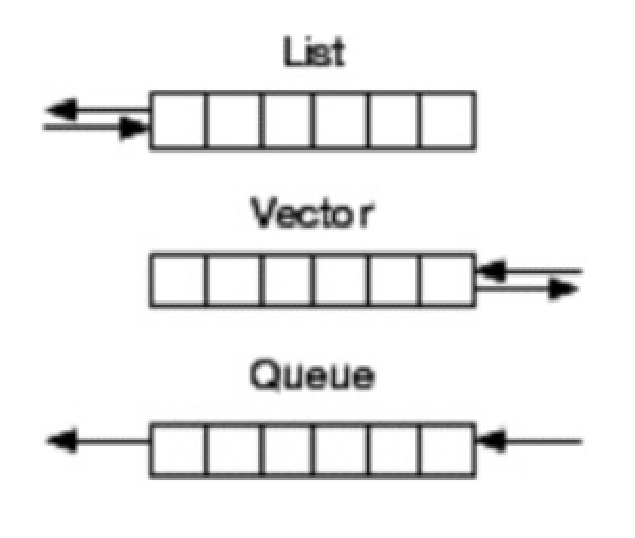
\includegraphics[width=5cm]{fig_02_001.eps}


他のすべてのコアコレクションと同様に、キューは不変の永続的なコレクションであり、リストやベクトルを扱うのと同じ関数をすべてサポートしています。以下は、ランチカウンターをキューで実装する方法です。

\begin{lstlisting}[numbers=none]
(def new-orders clojure.lang.PersistentQueue/EMPTY)

(defn add-order [orders order]
  (conj orders order))

(defn cook-order [orders]
  (cook (peek orders))
  (pop orders))
\end{lstlisting}

Clojureはリテラルなキューの構文やコンストラクタを提供しません。新しいキューを作成するには、静的な空のインスタンス \texttt{clojure.lang.PersistentQueue/EMPTY} で開始します。\texttt{add-order}では、vectorのように最後に新しい要素を追加するために\texttt{conj}を使用するだけです。\texttt{cook-order}では、最初の順序を見るために\texttt{peek}を使い、最初の順序以外を返すために\texttt{pop}を使います。

待ち行列の実装は、順序の追加と、待ち行列に入れられた順序での順序の削除の両方において効率的です。これは、この仕事に適したツールです。

次に、コレクションにデータを追加する処理を最適化する方法を考えてみましょう。


\subsection{一括インポート}

Clojureの永続的なコレクションは、イミュータブルです。効率化のために、\texttt{conj}や\texttt{assoc}のような関数で要素を追加すると、新しい不変の構造が作成されますが、その前と後のバージョンは通常そのデータの多くを共有します。コレクションは不変なので、これは安全に実行でき、データをコピーするよりもはるかに高速です。しかし、Clojureは制御されたコンテキストでミュータビリティを活用することで、より効率的にコレクションを埋める方法があります。

典型的なケースは、カタログアイテムのインポートです。アプリケーションが記録システムに直接アクセスできない場合、そのシステムからのエクスポートは、開始時にアプリケーションにインポートすることができます。カタログが変更されると、定期的な更新が必要になることは容易に想像できる。大規模なカタログの場合、その処理には時間がかかることがあります。

アプリケーションの起動時に呼び出される典型的なインポートを考えてみましょう。


\begin{lstlisting}[numbers=none]
(defn import-catalog [data]
  (reduce #(conj %1 %2) [] data))
\end{lstlisting}

変更できるようにして、誰にも知られずに多くの修正を加えることができたらどうでしょうか。Clojureのトランジェントがこれを可能にしてくれます。限られたスコープ内で、Clojureのコレクションを変更させることができます。

transientを呼び出すと、mutableバージョンのvector、hash-map、hash-setが得られます(オリジナルはimmutableのままです)。トランジェントコレクションはconjやassocのような永続的な変更関数では変更できません。 トランジェントコレクションにはインスタンスを変更する同等の関数セットがあり、すべて「\texttt{!}」接尾辞がつきます: \texttt{conj!}、 \texttt{assoc!}、などなどです。 読み込みインターフェイス(\texttt{get}、\texttt{contains?}など)は変更されずに動作し続けます。変更が完了したら、\texttt{persistent!}を呼んで、永続的なコレクションに戻ります。

以下は、transientコレクションを代わりに使用する\texttt{import-catalog}の更新版です。

\begin{lstlisting}[numbers=none]
(defn import-catalog-fast [data]
  (persistent!
    (reduce #(conj! %1 %2) (transient []) data)))
\end{lstlisting}

また、\texttt{item-data}にベクターのベクターとして読み込まれた約100万点のカタログアイテムをインポートしているときの速度を、時間を使って2つのバージョンの性能差を確認することができます。

\begin{lstlisting}[numbers=none]
catalog-import.core=> (time (import-catalog item-data)))
"Elapsed time: 129.602 msecs"
catalog-import.core=> (time (import-catalog-fast item-data)))
"Elapsed time: 110.104 msecs"
\end{lstlisting}

トランジェントは、バルクインポートを行う際に大きな力を発揮します。Clojureのinto関数が変換コレクションを取り、それがトランジェントにできるかどうかを判断するのはこのためです。もしそうなら、出力コレクションは自動的にトランジエントにされ、トランジエント関数を使用して充填され、永続的なコレクションに戻されます。

リストとベクター内の要素は、通常、更新されない。その代わり、シーケンシャルなコレクションでは、コレクションの挿入ポイントで要素の追加と削除を行うことがほとんどです。しかし、マップの内部内容は頻繁に更新され、マップはいくつかの一般的な方法で変換される必要がある。

\subsection{マップの更新}

マップを修正する基本的なツールは\texttt{assoc}と\texttt{dissoc}です。 \texttt{assoc}関数はキーに新しい値が供給されると、その値を更新します。Clojure 1.7では、関数の適用に基づいてキーの値を変換することができる\texttt{update}関数が追加されました。

例えば、宇宙シミュレーションの惑星の1つを記述するエンティティ(適切なマップ・インターフェイスも実装しています)を考えてみましょう。



\begin{lstlisting}[numbers=none]
(def earth {:name       "Earth"
            :moons      1
            :volume     1.08321e12 ;; km^3
            :mass       5.97219e24 ;; kg
            :aphelion   152098232  ;; km, farthest from sun
            :perihelion 147098290  ;; km, closest to sun
           }
\end{lstlisting}

ユーザーがシミュレーションに月を追加した場合の効果を調べるための機能を追加することを検討します。\texttt{update}関数を使って、月の数を増やす\texttt{inc}関数を適用することができます。


\begin{lstlisting}[numbers=none]
(update earth :moons inc)
\end{lstlisting}

\texttt{update}関数は、コレクション内の値に関数を適用し、その結果として更新されたコレクションを受け取るという処理をカプセル化したものです。

時には、マップ内の1つの値だけでなく、多くの値を同時に更新する必要があります。多くの場合、実体を表すマップは、CSVファイル、JSONデータ、データベースなどの外部データソースから取り込まれます。キーはキーワードではなく文字列であったり、キーワードが間違った名前空間や大文字小文字であったりと、求めるものと異なる形式であることがある。

Clojureコア・ライブラリには、マップ内のすべてのキーを更新するための単一の関数はまだ含まれていませんが、多くの外部ユーティリティ・ライブラリが解決策を提供しています。ここでは、多くの開発者が便利だと思う少数の関数を含む \texttt{Medley} ライブラリを使用します。

例えば、以下のような形式の文字列キーを持つJSONソースから惑星データを受信することを考える。


\begin{lstlisting}[numbers=none]
{"name" "Earth"
 "moons" 1
 "volume" 1.08321e12
 "mass" 5.97219e24
 "aphelion" 152098232
 "perihelion" 147098290}
\end{lstlisting}

\texttt{Medley}の\texttt{map-keys}関数を使って、このエンティティのキーを全て変更することができます。

\begin{lstlisting}[numbers=none]
(:require [medley.core :refer (map-keys)])
\end{lstlisting}

\begin{lstlisting}[numbers=none]
(defn keywordize-entity [entity]
  (map-keys keyword entity))

(keywordize-entity {"name"   "Earth"
                    "moon"   1
                    "volume" 1.08321e12
                    "mass"   5.97219e24
                    "aphelion" 152098232
                    "perihelion" 147098290})
;; {:name "Earth",
;;  :moons 1,
;;  :volume 1.08321E12,
;;  :mass 5.97219E24,
;;  :aphelion 152098232,
;;  :perihelion 147098290}
\end{lstlisting}

おそらくもっと一般的なのは、マップをインデックスとして使用する場合、1回の呼び出しですべてのマップの値を更新する必要があることでしょう。\texttt{Medley}ライブラリには、この目的のために\texttt{map-vals}関数も用意されています。

モデリングの関係で考えたレシピのインデックスがレシピ識別子からレシピへのマップであったことを思い出してください。もし私たちがインデックス内のすべてのレシピにカロリー情報を追加する必要があるならば、次のように\texttt{map-valsas}を使うことでレシピのインデックスを更新することができます。レシピの総カロリー数を生成できる\texttt{compute-calories}関数を持っていると仮定します。

\begin{lstlisting}[numbers=none]
(:require [medley.core :refer (map-vals)])
\end{lstlisting}


\begin{lstlisting}[numbers=none]
(defn- update-calories
  [recipe]
  (assoc recipe :calories (compute-calories recipe)))

(defn include-calories
  [recipe-index]
  (map-vals update-calories recipe-index))
\end{lstlisting}

まず、\texttt{update-calories}ヘルパー関数を定義します。これは、新しい\texttt{:calories}フィールドを計算し、単一のレシピに関連付けるために使用されます。それから、\texttt{include-calories}で、マップのすべての値にこの関数を適用するために\texttt{map-vals}を使用します。
   
マップのすべてのキーや値を更新するこれらの単純な関数は驚くほど便利で、ほとんどのプロジェクトは最終的にこれらのユーティリティを書いたり、含めたりしています。\texttt{Medley}では、これらの関数の実装にトランジェントを使用してパフォーマンスを向上させています。トランジェントの利点は、Bulk Importでご覧いただいたとおりです。

\texttt{Medley}には他にも、\texttt{filter-keys}、\texttt{filter-val}、\texttt{remove-keys}、\texttt{remove-val}という便利なマップ変換関数がいくつかあります。これらは、述語関数(ブール値を返す)を適用した結果に基づいて、マップエントリのサブセットを保持または削除することができます。

さて、コレクションを選んでデータを入れたら、次はそこからデータを取り出す方法を考えましょう。

 % Updating Collections
\section{コレクションにアクセスする}

コレクションの目的はデータを保存することですが、データをコレクションから取り出せてこそ、コレクションは役に立ちます。まず、キーによる索引検索をサポートするコレクションを考えてみましょう。

\subsection{インデックス付きアクセス}

Clojureで提供されるインデックス付きコレクションは、マップとベクターの2つです。ベクターは0ベースのインデックスを使用し、インデックスから要素への連想コレクションとして扱われます。ドメインをモデリングしているときに見たレコードもマップインターフェースを実装しており、インデックス付きコレクションとして扱うことができます。

インデックス付きコレクションは3つのメソッドで検索をサポートする。1つ目は、コレクションとキーを指定して\texttt{get}関数を呼び出す方法である。2つ目は、コレクションそのものをキーとともに呼び出す方法である。3つ目は、コレクションをキーワードやシンボルで呼び出す方法です。以下は、3つの方法の例である。

\begin{lstlisting}[numbers=none]
(def earth {:name "Earth" :moons 1})

(get earth :name) ;; (1) using get
(earth :name) ;; (2) invoking the map
(:name earth) ;; (3) invoking the keyword key
\end{lstlisting}

これらの3つの方法はすべて典型的なClojureプログラムで使用されますが、それぞれトレードオフが異なり、状況によって好まれる方法が異なります。

エンティティ(マップまたはレコード)については、関数としてキーワードを呼び出すことが好ましい方法であり、このスタイルの検索は広く使用されています。関数としてのキーワードキーの使用は、他の関数を入力として受け取るClojureライブラリの多くの関数とうまく連動します。

マップがデータの定数ルックアップ・テーブルとして、またはキーから値への関数として使用されている場合、マップを関数として呼び出すのが一般的です。この呼び出しスタイルの欠点は、呼び出されるマップが\texttt{null}の可能性がある場合、\texttt{NullPointerException}が発生することです。このため、この呼び出しスタイルは、\texttt{def}を使用して、決して\texttt{null}にならない一定のグローバルマップを作成した場合によく見受けられます。レコードは呼び出すことができないので、この方法では呼び出すことができないことに注意してください。

何が起こっているのかが不明な場合は、\texttt{get}を直接呼び出すと便利です。例えば、マップを作成する関数が使われているとき、関数の戻り値がたまたまルックアップテーブルであった場合に呼び出すと混乱することがある。

例えば、ここにある \texttt{opposite-colors} 関数は、特定のパレットにある色と対照的な色のマッピングを返します。

\begin{lstlisting}[numbers=none]
(defn opposite-colors
  "Compute an opposite-color mapping for a given palette."
  [palette]
  ;; This function should compute the mapping for the palette and
  ;; return a map like this with many entries: {:magenta :green}
  )
\end{lstlisting}

それに対する呼びかけを紹介します。

\begin{lstlisting}[numbers=none]
((opposite-colors palette) :magenta) ;; ok, but confusing
(get (opposite-colors palette) :magenta) ;; less confusing
\end{lstlisting}

最初の呼び出しの例は \texttt{opposite-colors} が返すマップを直接呼び出していますが、多くの Clojure 読者はこの使い方につまずき、何が起こっているのか不思議に思ってから解決することでしょう。一般的に、式の右側で閉じ括弧を山ほど見ることはよくありますが、左側で同じことを見ることは比較的まれです。関数を呼び出して、その戻り値をすぐに呼び出すということはほとんどありません。

2番目の呼び出しの例では、代わりに明示的にget関数を使用しています。これは、読者に対して、\texttt{opposite-colors}から返される値がマップであることを強く知らせるものです。このコードでは、\texttt{opposite-colors}が\texttt{nil}を返す場合にも対応しており、その場合は\texttt{get}も\texttt{nil}を返します。

マップから単一の値を取り出すこれらの方法に加えて、時にはサブマップを取り出し、エントリーの部分的なセットを選択することが有用である。Clojureはこの目的のために\texttt{select-keys}関数を提供します。この関数は常にハッシュ・マップを返し、ソース・タイプ(レコード、ソート・マップなど)のマップは返しません。

もし、私たちが宇宙シミュレーションからデータのエクスポートを準備していたなら、最も重要なキーのうちのいくつかだけを選択して、情報の一部を省略した簡略化したエクスポートを提供することができます。

\begin{lstlisting}[numbers=none]
(defn export-planet
  [planet]
  (select-keys planet [:name :moons]))
\end{lstlisting}

エクスポートされる惑星は、単純なマップになります。\texttt{\{:name "Earth" :moons 1\}} というシンプルなマップになります。次に、シーケンシャルなデータ構造の中のものを探すことに目を向けましょう。

\subsection{逐次探索}

前節で扱ったマップは、ある値を効率的に一定時間で調べたいときに常に理想的な選択肢となる。同様に、セットも\texttt{contains?}関数を使って、あるセットが特定の値を含んでいるかどうかを素早くチェックすることができます。しかし、\texttt{contains?}関数はリストやベクトル内の値で項目を探すのには使えません。

順番に並んだコレクションが必要で、かつそのコレクションの中の値も見つける必要がある場合、コレクションを順番に検索して一致するものを見つける方法が必要です。この検索にかかる時間は、コレクションのサイズに比例することに注意する必要があります。

Clojureで見られる逐次探索の最も一般的なテクニックの1つは、some関数を使うことです。この関数はコレクションの各要素に対して述語を評価し、最初の論理的に真となる値(元の要素ではありません)を返します。これは単純な値のコレクションで最も便利です。

\begin{lstlisting}[numbers=none]
(def units [:lb :oz :kg])

(some #{:oz} units)
;;=> :oz
\end{lstlisting}

\texttt{some}と一緒に使われている述語は、1つの値を含むセットです。ここでは、前のセクションと同じコレクション呼び出しのスタイルを活用し、ユニットベクタの各要素を順番に持つ関数としてセットを呼び出しています。マッチングが成立すると、その値が返されます。結果は真理値として使用することができます。マッチしない場合は、\texttt{nil}が返される。

この目的のために\texttt{some}を使うことはよくあるが、論理的に偽である\texttt{nil}や\texttt{false}を探すという特殊なケースで破綻する。

論理的に偽の値の検索をサポートし、早期に終了する比較的効率的な線形探索の実装は以下のように定義できる。

\begin{lstlisting}[numbers=none]
(defn contains-val?
  [coll val]
  (reduce
    (fn [ret elem] (if (= val elem) (reduced true) ret))
    false coll))

(contains-val? units :oz)
;;=> true
\end{lstlisting}

\texttt{reduce}と\texttt{reduced}の使い方は、Reducing to a Valueで詳しく説明します。

Clojureが提供するコレクションをどのように活用するか決めたところで、独自のコレクションを構築する方法を検討することで、自分のアプリケーションに固有の問題を解決する方法も考えたいと思います。

 % Accessing Collections
\section{カスタムコレクションの構築}

Clojureのコレクションがどれもあなたの問題に適していない場合、あなた自身でロールバックする必要があるかもしれません。標準のコレクションと同様に、カスタム・コレクションはClojureコア・ライブラリでシームレスに使用できます。カスタム・コレクションを構築するには、Clojureが内部で使用するtraitインタフェースを実装するためにdeftypeを使用することが必要です。

\subsection{コレクションの特徴}

Clojureが使用できるコレクションを構築したい場合、Clojureがコレクションとどのように相互作用するかをより深く理解する必要があります。コレクションとシーケンスライブラリは、Clojureに含まれる特定の実装ではなく、主要な抽象化を定義する特質の一般的なセットに基づいています。Clojureのコレクション特質は、Javaインタフェースを使用して内部的に実装されています。

述語関数は、コレクション実装上のClojureコレクションの特徴の存在を検出するためにClojureで提供されます。述語関数は質問をし、ブール値の答えを返しますが、Clojureでは慣例的に名前に末尾の\texttt{?}をつけます。

Clojureの述語コレクション関数には、以下のようなものがあります。


\begin{itemize}
\item \texttt{counted?}--コレクションは一定時間内に数えることができるか?
\item \texttt{sequential?}--値が特定のトラバース可能な順序で格納されているか?
\item \texttt{associative?}--コレクションはキーと値の間の関連性を保存しているか?
\item \texttt{reversible?}--コレクションは可逆的か?
\item \texttt{sorted?}--コレクションはソートされた順序で管理されているか?
\end{itemize}

これらの特質は、以下のJavaインタフェースに対応している。\texttt{Counted}、Sequential、\texttt{Associative}、\texttt{Reversible}、\texttt{Sorted}です。その他の内部インターフェースは、コアコレクションインターフェースの構造や、パブリックコレクション関数の下で使われる主要なメソッドを定義している。

カスタムコレクションを構築するとき、実装したいClojure関数から、その関数をサポートするためにコレクションに必要な実装のJavaインタフェースまで、逆算する必要があります。

この図は、Clojure関数(右の列)からJavaメソッド(左の列)へのマッピングを提供します。各インターフェースに対する述語関数は、各Javaインターフェース名の下に記載されています。

\begin{figure}[h]
\centering
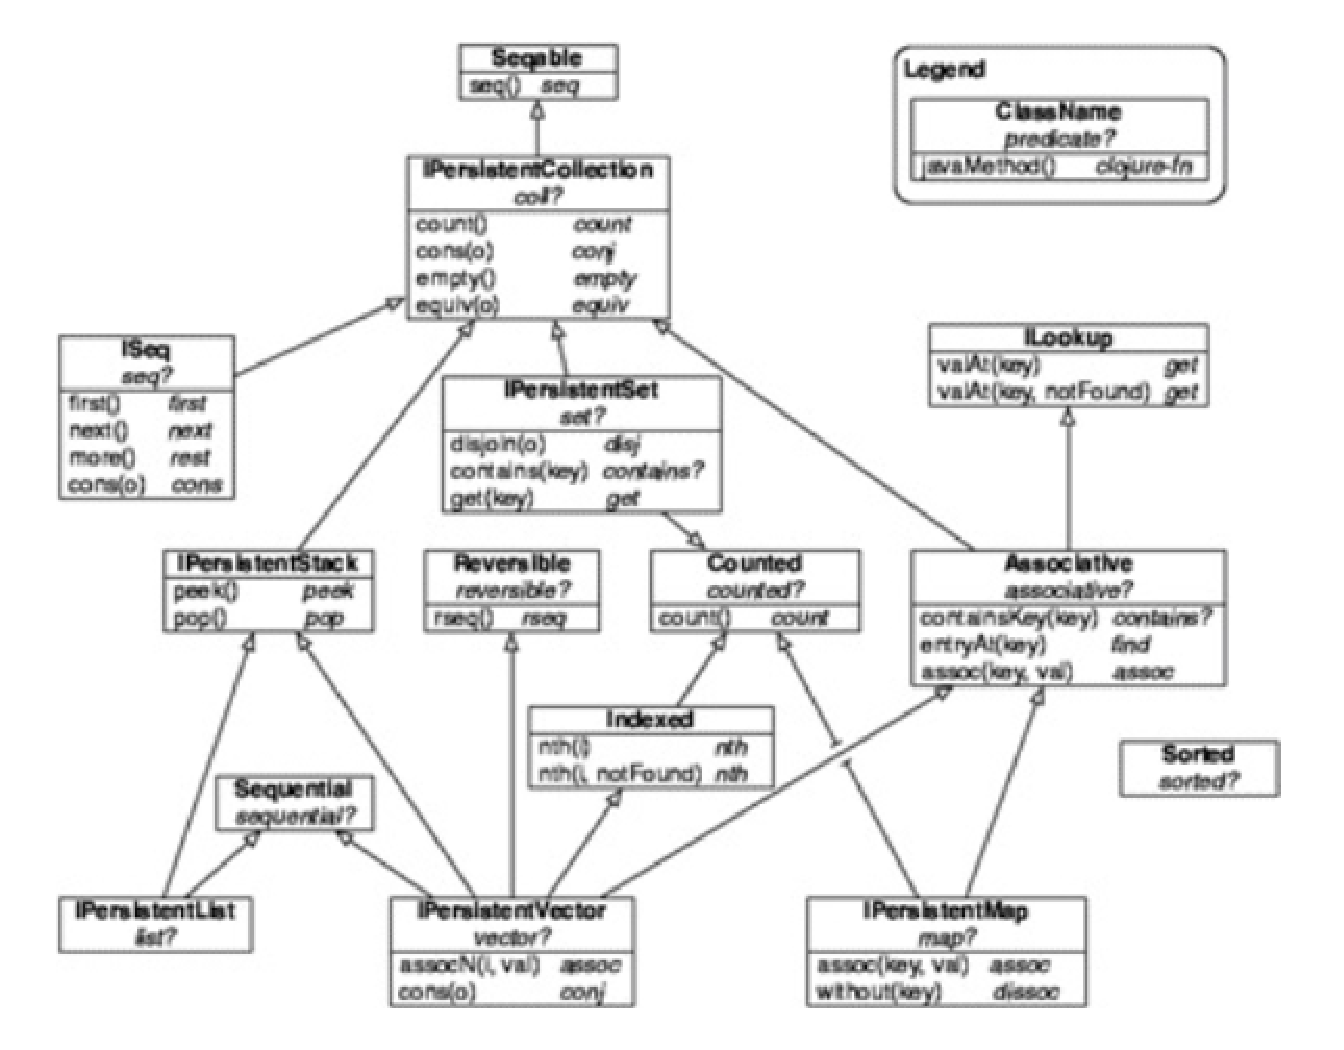
\includegraphics[width=8cm]{fig_02_002.eps}
\caption{Clojure関数とそれに対応するJavaメソッド}
\end{figure}

Clojureで意図した使用方法とマッピング図を用いて、目的を満たすカスタムコレクションを構築する方法を見てみましょう。

\subsection{deftypeでコレクションを作成する}

まず、このコレクションが何をする必要があるのかを考えてみましょう。a と b と呼ぶ 2 つの値を保持するカスタム \texttt{Pair} クラスを実装するつもりです。\texttt{Pair} 型は \texttt{seq}、\texttt{count}、\texttt{nth}、および \texttt{get} で動作するようにしたいと思います。図を見てみると、\texttt{Seqable}、\texttt{Counted}、\texttt{Indexed}、\texttt{ILookup}を実装する必要があることがわかります。

カスタムデータ構造を実装するには、\texttt{deftype}マクロを使用します。
これは\texttt{defrecord}に似ているが、より多くの機能を提供し、マップとの組み込みの類似性は少ない。例えば、\texttt{deftype}は\texttt{record}と同じように型とコンストラクタ関数を取得しますが、自動的にマップのように動作するわけではありません。\texttt{deftype}では、必要であればマップのように振舞うために適切なインタフェースを実装するのは我々の責任である。型はまた、他のClojure構成要素では利用できない、mutableフィールドやunsynchronizedフィールドのような特殊な機能のサポートを持っています。

\texttt{Pair}が\texttt{deftype}としてどのように見えるか見てみましょう。

\begin{lstlisting}[numbers=none]
(ns ch2.pair
  (import [clojure.lang Counted Indexed ILookup Seqable]))

(deftype Pair [a b]
  Seqable
  (seq [_] (seq [a b]))

  Counted
  (count [_] 2)

  Indexed
  (nth [_ i]
    (case i
      0 a
      1 b
      (throw (IllegalArgumentException.))))
  (nth [this i _] (nth this i))

  ILookup
  (valAt [_ k _]
    (case k
      0 a
      1 b
      (throw (IllegalArgumentException.))))
  (valAt [this k] (.valAt this k nil)))
\end{lstlisting}

\texttt{deftype}の内部では、実装される各インターフェースをリストアップし、次にメソッドの実装を提供します。

これでREPLから\texttt{Pair}型を利用することができるようになりました。

\begin{lstlisting}[numbers=none]
user> (use 'ch2.pair)
nil
user> (def p (->Pair :a :b))
#'user/p
user> (seq p)
(:a :b)
user> (count p)
2
user> (nth p 1)
:b
user> (get p 0)
:a
user> p
#object[ch2.pair.Pair 0x39b4cec7 "ch2.pair.Pair@39b4cec7"]
\end{lstlisting}

\texttt{p}を直接見ようとするまではうまくいっていたのですが、これから修正します。

\subsection{型のカスタム表示}

先ほど見たように、型にはクラス名と識別子を含むあらかじめ定義された表示フォーマットがあります。私たちの型の表示形式には、インスタンスデータが含まれるようにしたいのです。リーダーはClojure内部のコンポーネントで、文字列を読み込んでClojureデータを返します。理想的には、リーダーによって読むことができるフォームで私たちの型を表示したいです -- これはリテラル値として私たちに完全なラウンドトリップ能力を与えます。

表示装置は、カスタムプリンターを供給するフックを定義するマルチメソッドを持つオープンシステムです。考慮すべきは、\texttt{print-method}(ユーザのために表示するときに呼び出される)と\texttt{print-dup}(リーダーのために表示するときに呼び出される)の2つのフックである。例えば、Clojure文字列は、\texttt{print-method}では周囲の引用符なしで表示されますが、 \texttt{print-dup}では周囲の引用符で表示されます。

私たちの目的のために、私たちはどちらの場合でも同じようにペアタイプを表示したいので、単に\texttt{print-method}を呼び出すために\texttt{print-dup}を実装することにします。

\begin{lstlisting}[numbers=none]
(defmethod print-method Pair
  [pair ^Writer w]
  (.write w "#ch2.pair.Pair")
  (print-method (vec (seq pair)) w))

(defmethod print-dup Pair
  [pair w]
  (print-method pair w))
\end{lstlisting}

そのため、今回のプリンターでは、\texttt{Pair}データをベクターに変換し、既存のベクター用\texttt{print-method}に対応させることで簡略化しています。試してみましょう。

\begin{lstlisting}[numbers=none]
user> (use 'ch2.pair.print)
nil
user> (->Pair 1 2)
#ch2.pair.Pair[1 2]
user> #ch2.pair.Pair[3 4]
#ch2.pair.Pair[3 4]
\end{lstlisting}

Clojureリーダーはこの形式を使用してJavaオブジェクトを構築するため、今回表示する構文は特別に選択されました。フォーマットは\tex{#class\[args\]}です。前のコードでは、コンストラクタ・クラスの構文を REPL に置くと、リーダーはそれを \texttt{Pair} オブジェクトに読み込んで、プリンタは私たちの \texttt{print-method} プリンタを使用して結果のオブジェクトを表示します。

 % Building Custom Collections
\section{まとめ}

これで、ドメインモデルの内部と外部の両方でコレクションを使用して、エンティティと値の両方を収集する方法について完全に理解しました。Clojureアプリケーションのデータのほとんどは、ここで説明したコレクション以外から構築されていません。時折、特殊な考慮事項やパフォーマンスを最大化するために、独自のコレクションを構築することが有用であることが分かるでしょう。

第4章「状態、アイデンティティ、および変更」で状態をどのように管理することを期待するかについて、段階を踏んでいます。この章で説明した概念と同様に、状態管理は不変の値と純粋な変換関数の基礎に大きく依存しています。

しかし、まずはコレクションと関数に関する知識を活かして、データを処理する能力をどのように拡張するかに焦点を当てます。これまでは、主にコレクション・レベルで、単一の値やエンティティを変更してきました。次に、範囲を広げてシーケンスについて説明します。

シーケンスとは、リストやベクターなどのコレクションをシーケンシャルなデータ構造のように扱えるようにするための一般化表現です。Clojureのデータ変換機能のほとんどは、特定のコレクションに縛られることなく、このより一般的な抽象化の上に構築されています。Clojureのデータ変換関数は、強力で再利用可能なClojureアプリケーションを書くための重要な部分です。
 % Wrapping Up

     
    
         
\chapter{シーケンシャルデータの処理}

% \section{値のマッピング}

アプリケーションの中でデータが移動するとき、ある部分が別の形でデータを必要とすることはよくあることです。あるサブシステムは、30列のスプレッドシートから30個のキーを持つ汎用マップにデータをインポートする。別のサブシステムでは、5列のデータをエンティティの形で必要とし、さらに別のシステムでは、一連のエンティティから1つのフィールドのみを必要とし、計算を実行したり画面に表示したりします。

これらのユースケースはすべて、シーケンシャルなソースにある値をある形式から別の形式に変換する必要があります。Clojureでは、map関数はシーケンスの各要素に関数を適用して、その結果の新しいシーケンスを生成するために使用されます。

例えば、宇宙シミュレーションの各惑星エンティティの軌道周期を抽出して画面に表示する必要があるとします。入力は惑星のベクターであり、これはシーケンス、つまり論理的には値のリストとして扱われます。

このシーケンシャルな惑星の集合を、各惑星の軌道周期のシーケンシャルな集合に変換する必要がある。軌道周期とは、惑星が太陽の周りを完全に1周するのにかかる時間である。例えば、地球の場合、公転周期は約365.25日である。

$$
\mu = GM
$$

$$
T = 2 \pi \sqrt{\frac{a^3}{\mu}}
$$

任意の惑星の公転周期を計算する関数を書くことができる。この関数の詳細を理解することは、特に重要ではありません。(もし興味があれば、ここにその方程式を示す。Tは惑星の公転周期、$μ$は標準的な重力パラメータです)。

この値は、惑星だけでなく、中心星の質量にも依存する。公転周期を計算する関数は、惑星と恒星の質量を引数として受け取り、公転周期を返す。



\begin{lstlisting}[numbers=none]
(defn semi-major-axis
  "The planet's average distance from the star"
  [p]
  (/ (+ (:aphelion p) (:perihelion p)) 2))

(defn mu [mass] (* G mass))

(defn orbital-period
  "The time it takes for a planet to make a complete
  orbit around a mass, in seconds"
  [p mass]
  (* Math/PI 2
    (Math/sqrt (/ (Math/pow (semi-major-axis p) 3) (mu mass)))))
\end{lstlisting}

さて、変換関数ができたので、それを使って惑星のコレクションを公転周期のコレクションに変換しなければなりません。Clojureのマップ関数は、惑星のベクターに変換関数を適用して、連続したソース内のすべての値を新しい値に「マップ」する方法です。

1つの引数(値)を取り、新しい値を返す変換関数が必要です。しかし、\texttt{orbital-period}関数は2つの引数を取る関数なので、今ある関数を正しい形(1つの引数)の変換関数にラップする必要があります。これは、定数値(太陽質量)が現在の関数スコープで利用可能な無名関数を使用することでしばしば行われる。

\begin{lstlisting}[numbers=none]
(defn orbital-periods
  "Given a collection of planets, and a star, return the
  orbital periods of every planet."
  [planets star]
  (let [solar-mass (:mass star)]
    (map (fn [planet] (orbital-period planet solar-mass))
         planets)))
\end{lstlisting}

この例では、惑星のコレクションと星を受け取り、星から太陽質量を取り出しています。そして、惑星を受け取り、その惑星と太陽質量を用いてorbital-period関数を呼び出す無名関数でmapを呼び出すことができます。map関数は、この関数をすべての惑星に適用しながらコレクションを走査し、結果を一連のシーケンスにまとめて最後に返します。

mapが何をしているのか、コレクションの世界からシーケンスの世界へどのように入り込んでいるのか、もっと詳しく見ていきましょう。


\subsection{シーケンス処理}

 mapの仕事は、シーケンスのすべての値に関数を適用することである。ここでは Clojureがこの関数を実装する方法の簡略版です。このバージョンを \texttt{simple-map} と呼ぶことにします。


\begin{lstlisting}[numbers=none]
(defn simple-map
  "Map f over the elements of coll."
  [f coll]
  (when (seq coll)
    (cons (f (first coll))
          (simple-map f (rest coll)))))
\end{lstlisting}

この実装はClojureのシーケンスAPIを使って書かれており、主に\texttt{seq}, \texttt{first}, \texttt{rest}, \texttt{cons}関数から構成されています。\texttt{seq}関数は、コレクションが少なくとも1つの要素からなるシーケンスであるかどうかを尋ねます。もしそうなら,それが返され,そうでなければ,nilが返される.この結果は真か偽かを表すので、この関数はしばしば終了の条件チェックに使われる。

マッピングされるコレクションがより多くの要素を持つ場合、\texttt{cons}関数を適用する。\texttt{cons}関数は、値を含むセルと、次のセルへのポインタを構成する。これは典型的なリンクリストのデータ構造であり、値を含む一連のセルである。最初のセルの値は、変換関数fをコレクション内の最初の値に適用したものとして定義される。残りのセルは、同じ関数と入力コレクションの残りを渡して、この関数を再帰的に呼び出すことによって定義される。

この再帰的なシーケンスの定義は、シーケンシャルなコレクション(リストまたはベクタ)に適用されるが、そのデータ構造の実装方法の詳細には一切依存しない。シーケンスAPIを実装するためには、参加者(participant)は次の要素が存在するかどうかをチェックし、最初の要素を返し、残りの要素に対して新しい実体を返すことができればよいのである。つまり、シーケンスとはコレクションの論理的な見方である。

軌道周期の例では、シーケンシャルなコレクションやシーケンスAPIの他の実装を渡しても、\texttt{map}は動作する。シーケンスの抽象化により、汎用的な\texttt{map}関数が様々なデータソースで動作するようになった。

一般にシーケンス関数は、seqable(\texttt{seq}を適用するとシーケンスを生成できるもの)を入力として受け取り、同じものを返すと考えられています。しかし、この場合の結果は永続的なリストとなり、関数に渡されたベクトルほど高速でもメモリ効率も良くはありません。Clojureはこの特殊なケースのために、特別なmapv関数を提供します。mapv関数はmapと使い方は同じですが、特にベクトルを受け取って返します。

これは、ほとんどのシーケンス関数の典型的な側面を強調しています。入力ソース(シーケンス対ベクトル)の反復、変換の適用(\texttt{f}関数の適用)、結果に対する何らかの処理(リストの構築またはベクトルの構築)を組み合わせています。

この3つを組み合わせると、シーケンスの使い方が制限されます。しかし シーケンス入力は抽象化されたものであり,事実上あらゆるソースで実装可能である.同様に,この関数は出力シーケンスしか生成しないので,コレクションに挿入したり,通信チャネルに値を渡したりするには,別のバージョンが必要になる.これらの部品を分解するために、トランスデューサーが導入された。

\subsection{トランスデューサー}

トランスデューサの定義では、入力値がどこから来て、その出力がどのように使われるかを指定することを避け、代わりにトランスデューサが行う実際の作業のみを定義します。\texttt{map}の場合、トランスデューサの仕事は関数がすべての要素に適用されるようにすることです。その本質は、入力要素がコレクション、シーケンス、ソケット、キューのどれであっても、また、出力がコレクションに追加されるかファイルに保存されるかにかかわらず、同じです。

トランスジューサの実装はやや複雑なので説明しませんが、どのように作成され適用されるかを見ることは重要です。マップトランスジューサを作るには、\texttt{map}を呼び出すときに入力コレクションを省略します。

\begin{lstlisting}[numbers=none]
(defn orbital-period-transformation
  "Create a map transformation for planet->orbital-period."
  [star]
  (map #(orbital-period % (:mass star))))
\end{lstlisting}

この変換は、様々な入力ソースと出力条件に対して使用することができる。前の版の\texttt{map}と同様の出力シーケンスを生成するために、この変換とシーケンス関数を使用することができます。

\begin{lstlisting}[numbers=none]
(defn orbital-periods
  [planets star]
  (sequence (orbital-period-transformation star) planets))
\end{lstlisting}

\texttt{mapv}版のような出力ベクトルを作成する場合は、以下のようにします。

\begin{lstlisting}[numbers=none]
(defn orbital-periods
  [planets star]
  (into [] (orbital-period-transformation star) planets))
\end{lstlisting}

あるいはリストを作成する。

\begin{lstlisting}[numbers=none]
(defn orbital-periods
  [planets star]
  (into () (orbital-period-transformation star) planets))
\end{lstlisting}

\texttt{sequence}と\texttt{into}を用いた\texttt{orbital-periods}は、要素の実現方法が異なるため、遅延の概念に関わる。




\subsection{遅延性}

ほとんどのClojureシーケンス関数は、関数が評価されるときに変換を実行しない、遅延シーケンスを生成します。その代わり、遅延シーケンスは、シーケンスの消費者が必要とするときだけ評価されます。オリジナルのシーケンス版である \texttt{map} とシーケンス付きトランスデューサーは、どちらも必要に応じて計算される遅延シーケンスを生成します。

遅延シーケンスは、決して計算される必要のない作業を避けることができるという点で有用です。この場合、軌道周期の遅延シーケンスを消費するコードがなければ、計算する必要はないでしょう。遅延シーケンスは、フィボナッチ・シーケンスや素数シーケンスのような無限の値の並びを表現するのにも便利です。我々は、計算のためにそれらすべてを見ることは決してない(ありえない)。しかし、無限シーケンスとして定義することで、目的に応じて必要な数だけ取ることができる。

これに対して、\texttt{into} は出力全体を熱心に計算し、それを返す関数である。熱心な計算が便利なのは、計算がいつ行われるかを簡単に推論できるようになるからです。これにより、トランスデューサーで使用されるリソースの管理や廃棄が容易になったり、計算が行われるタイミングを正確に管理することができます。

さらに、\texttt{into}で行われる熱心な計算は、しばしばメモリと時間の両面でより効率的です。シーケンスは計算された値をキャッシュしますが、トランスデューサーの熱心なアプリケーションは、中間値を割り当てることなくソースコレクションに対して実行できることがよくあります。

\texttt{into}関数は、より一般的な\texttt{reduce}関数で実装されており、入力コレクションを値に還元します。









\begin{lstlisting}[numbers=none]

\end{lstlisting}




 % Mapping Values
% \section{値への還元}

\texttt{reduce}関数は、蓄積された値とコレクションの次の要素に関数を繰り返し適用することで、コレクションを値に還元する関数です(オプションの初期値を使用)。\texttt{into}関数は、コレクションを単純な値ではなく、別のコレクションに還元する特殊なケースです。

例えば、宇宙シミュレーションで、太陽系のすべての惑星にある月の総数を計算することを考えてみましょう。まず、各惑星の月の数を抽出し(マッピング変換)、それらを\texttt{+}関数で一つの値(合計)に還元する必要があります。\texttt{reduce}関数は、収集変換と削減のステップを組み合わせるためによく使われる。

\texttt{map}と\texttt{reduce}を使って、惑星の集合の総和を計算することができる。



\begin{lstlisting}[numbers=none]
(defn total-moons
  [planets]
  (reduce + 0 (map :moons planets)))
\end{lstlisting}

この関数は、各 \texttt{Planet} レコードに適用する関数として \texttt{:moons} というキーワードを使用して、惑星をマッピングします。その結果、各惑星の月の数を表す数値の列が生成されます。

次に、\texttt{reduce}はそれらの要素にそれぞれ+関数を適用し、初期蓄積値として0から始めます。

\texttt{reduce}はシーケンスではなく、値を生成するため、イーガーとなります。そのため、計算は\texttt{reduce}が実行されたときに行われます。

この変換は,トランスデューサーと類似の関数である\texttt{transduce}を使って計算することもできます.この関数は\texttt{reduce}とは異なり,入力ソースの各要素に適用するトランスデューサと,変換の出力値をどうするかを決定する\texttt{reduce}関数の2つの関数を受け取ります.トランスデューサーは意図的に、入力がどのように供給されるか(ここではソースコレクションから)と、その後に入力に対して何が行われるかの両方から変換を切り離すことを思い出してください。



\begin{lstlisting}[numbers=none]
(defn total-moons
  [planets]
  (transduce (map :moons) + 0 planets))
\end{lstlisting}


このバージョンは先行例と同じ要素を多く含み、表面的には多くの点で類似しています。しかし、このトランスデューサーのバージョンには、2つの潜在的な利点があります。まず、\texttt{(map :moons)} トランスデューサはここではインラインで使われていますが、別の関数として取り出して、今あるものでも将来作られるものでも、どんなトランスデューサのコンテキストでも再利用できる可能性があります。つまり、変換アルゴリズム(単純かもしれませんが)は、そのアルゴリズムの適用から抽象化されているのです。

第二に、ソースにトランスデューサを適用すると、ソースコレクションの単一のトラバーサルが生じます。このトラバーサルは、一連の値を構築するオーバーヘッドなしに自分自身を縮小する方法を知っているソースを利用できることがあります。

次の節で複数のトランスデューサーを合成する方法の例を示します。その前に、ソースのすべての要素を訪れることなく、早期にリダクションを停止する必要があるという特別なケースを考える必要があります。\texttt{Planet}レコードのリストが与えられた場合、特定の1つ、おそらく\texttt{Earth}と名付けられたものを見つけたいと思うかもしれません。この関数は以下のように実装できます。




\begin{lstlisting}[numbers=none]
(defn find-planet
  [planets pname]
  (reduce
    (fn [_ planet]
      (when (= pname (:name planet))
        (reduced planet)))
    planets))
\end{lstlisting}






 % Reducing to a Value
% \section{値のフィルタリングと削除}

惑星のコレクションではなく、太陽系内の全エンティティのコレクションを渡されることもある。その場合、月の総数を計算するには、惑星だけをフィルタリングして月の数を抽出し、月の総数を計算する必要がある。まずはシーケンスを使ってどのように見えるか見てみましょう。


\begin{lstlisting}[numbers=none]
(defn planet?
  [entity]
  (instance? Planet entity))

(defn total-moons
  [entities]
  (reduce + 0
    (map :moons
      (filter planet?
        entities))))
\end{lstlisting}


エンティティが惑星であるかどうかをテストする\texttt{planet?}ヘルパー関数を定義しました。Clojureでは、真偽の値を返す関数は述語と呼ばれます。それらはしばしば \texttt{?} で終わる名前を与えられます。一般的に、あなたが定義するほとんどのドメインは、いくつかのヘルパー述語を 持っています。

一連のシーケンス変換をネストするとき、しばしば、スレッドラストマクロ \texttt{->>} を使うと便利です。このマクロは、前の例のようにインサイドアウトではなく、一連の変換を順番に読むことができるようにコードを再構築する。

同じ例を \texttt{->>} で書き直すと、各式の結果を次の式の最後の位置に「通す」ようになります。すべてのシーケンス式は入力シーケンスを最終引数として受け取るので、ほとんどの入れ子になったシーケンス変換とうまく連動することができます。


\begin{lstlisting}[numbers=none]
(defn total-moons
  [entities]
  (->> entities
       (filter planet?)
       (map :moons)
       (reduce + 0)))
\end{lstlisting}

これで、\texttt{filter}、\texttt{map}、\texttt{reduce}の順に適用される関数をトップダウンで読むことができるようになりました。

トランスデューサーで同じ結果を得るには、最初の2つの変換(\texttt{filter}と\texttt{map})を合成して、\texttt{transduce}で適用する必要があります。各トランスデューサーはスタックのように前のものを包むので、スレッドラストマクロと同じトップダウンの適用順序で関数を構成するために \texttt{comp} を使うことができます。

\begin{lstlisting}[numbers=none]
(def moons-transform
  (comp (filter planet?) (map :moons)))

(defn total-moons
  [entities]
  (transduce moons-transform + 0 entities))
\end{lstlisting}

構成された変換を作成した後、\texttt{transduce} からそれを呼び出すのは簡単でした。ここでも、この関数のシーケンス版と比較して、いくつか注目すべき点があります。まず、合成変換は太陽系内の惑星から月だけを返します。この変換は、エンティティが別の入力ソースから来る別の計算で再利用することができます。

シーケンスバージョンでは、まずエンティティのコレクションを生成し、次に惑星だけの小さなシーケンスを生成し、最後に月の数のシーケンスを生成します。各中間シーケンスでは、オブジェクトが割り当てられ、メモリが消費される。Transducerバージョンでは、単一の複合変換を使用し、ソース入力にシングルパスで適用されます。ここでの節約はわずかですが、多数の変換と数千のエンティティを含む実際の使用では、パフォーマンスの向上は大きなものです。

しかし、他の使用例では、怠惰が重要な属性となり得ることを心に留めておいてください。そのような場合は、シーケンス版の方が好ましい。

コレクションをフィルタリングする関数には、\texttt{filter}の他に\texttt{remove}と\texttt{keep}があります。\texttt{remove}関数は\texttt{filter}の逆で、残すべき値ではなく、取り除くべき値を指定します。\texttt{keep}関数は、\texttt{map}と\texttt{filter}の機能を一つの便利なパッケージにまとめたもので、各要素に関数を適用し、\texttt{nil}でない結果を保持します。 % Filtering and Removing Values
% \section{takeとdrop}

述語に基づいてコレクションのサブセットを構築する代わりに、コレクションの先頭を取得または削除することがしばしば有用である。Clojureでは、\texttt{take}と\texttt{drop}関数がこれを達成することができます。例えば、外部ソースから太陽系エンティティのシーケンスを受け取る場合、次のような関数で結果のn番目のページを取得することができます。


\begin{lstlisting}[numbers=none]
(defn nth-page
  "sourceのn番目(0ベース)のpageに対して、
   page-sizeまでの結果を返す"
  [source page-size page]
  (->> source
       (drop (* page page-size))
       (take page-size)))
\end{lstlisting}

この関数は、まず要求されたページまでのページ数を落とし、次に要求されたページの集合を取り込む。この関数はシーケンスを使用し,要求されたページの結果を超える要素は実現しない.トランスデューサのフォームは、早期終了を知らせるために\texttt{reduced}を使用し、また要求された範囲を超えた結果を実現しないようにします。

ページを返すだけでなく、そのページと残りのコレクションの両方をさらなる処理のために必要とする場合もあります。split-at ヘルパー関数は \texttt{take} と \texttt{drop} の両方を実行し、両方をタプルとして返します。


\begin{lstlisting}[numbers=none]
(defn page-and-rest
  [source page-size]
  (split-at page-size source))
\end{lstlisting}

これは、最初のページと、最初のページ以外のすべてのベクターを返します。さらに処理を進めると、最初のページ以降の結果に対して再びこれを呼び出すことができる。

また、\texttt{take}と\texttt{drop}はカウントではなく述語で動作するバージョン、\texttt{take-while}と\texttt{drop-while}も使用できる。\texttt{split-with}関数は\texttt{split-at}と等価な述語です。

\texttt{take}と\texttt{drop}関数で要素のサブセットを選択する前に、コレクション内の要素の順序を指示するためにソートを組み合わせることはしばしば有用である。




 % Take and Drop
% \section{ソートと重複排除}

最も基本的なソート機能は \texttt{sort} で、デフォルトのコンパレータまたは必要に応じてカスタムのコンパレータでソートすることができます。例えば、これはアルファベット順で最初の5つの惑星名を取得します。


\begin{lstlisting}[numbers=none]
(take 5 (sort (map (:name planets))))
\end{lstlisting}

この例では、惑星の名前を取得し、その名前をソートしています。しかし、しばしば、元の実体を惑星名で並べ替えたいことがある。つまり、値を取り出すのではなく、各要素に適用される関数でソートしたいのです。これは\texttt{sort-by}で実現できる。


\begin{lstlisting}[numbers=none]
(take 5 (sort-by :name planets))
\end{lstlisting}

 % Sorting and Duplicate Removal
% \section{値のグループ化}

便利な\texttt{group-by}関数は、述語に基づいてデータをグループ化し、述語の結果とその結果にマッチするすべてのシーケンスのマップを返すことができます。例えば、惑星の最初の文字でインデックスを作成することができます。



\begin{lstlisting}[numbers=none]
(defn index-planets
  [planets]
  (group-by #(first (:name %)) planets))
\end{lstlisting}

この関数は、\texttt{E}, \texttt{J}, \texttt{M}, \texttt{N}, \texttt{S}, \texttt{U}, \texttt{V}をキーとするマップを返す。各値は、地球、木星、火星と水星、海王星、土星、天王星、金星の惑星エンティティのシーケンスである。

\texttt{group-by}の一般的な使用方法の1つは、含むコードで両方が必要な場合に\texttt{true}と\texttt{false}のキーのマップを返す述語と組み合わせて使用することです。

例えば、月のある惑星と月のない惑星を分けたい場合、述語は次のようになります。


\begin{lstlisting}[numbers=none]
(defn has-moons?
  [planet]
  (pos? (:moons planet)))
\end{lstlisting}

この述語は、マップ上で惑星を2つのバケツに分けるために使われる。


\begin{lstlisting}[numbers=none]
(defn split-moons
  [planets]
  (group-by has-moons? planets))
\end{lstlisting}

Clojureでシーケンシャルなデータを処理する一般的な方法のほとんどを示したので、より大きな例のコンテキストでそれがどのように見えるかを見てみましょう。 % Grouping Values
% \section{すべてをまとめる}

多くの場合、シーケンシャルデータの処理は同じようなパターンで行われます。

\begin{enumerate}
\item  どんな質問をしようとしているのかを把握する。このステップは、問題領域やビジネス領域に位置するため、最も困難な場合が多い。明確な質問があれば、Clojureはあなたが持っているデータを処理して答えを出すためのツールを提供します。それが次の3つのステップです。
\item  データをフィルタリングして、不要な要素を取り除く。
\item 要素を目的の形に変換する。
\item 変換された要素を答えに還元する。
\end{enumerate}


ショッピングカートの例で説明しましょう。オンラインストアでは、カタログ、つまり販売する商品のリストがあります。これらの商品は部門ごとに分けられています。顧客はそれらをカートに入れ、チェックアウトする。このプロセスで、請求記録が作成されます。あなたの顧客は、部門別の売上を要約したレポートを要求しています:すべての決済されたカートについて、部門ごとの総売上はいくらですか?

ドメインモデルは次のとおりです。


\begin{lstlisting}[numbers=none]
(require '[money :refer [make-money +$ *$]])

(defrecord CatalogItem [number dept desc price])
(defrecord Cart        [number customer line-items settled?])
(defrecord LineItem    [quantity catalog-item price])
(defrecord Customer    [cname email membership-number])
\end{lstlisting}

何度もチェックアウトを繰り返すと、カートには\texttt{\#Cart}レコードのベクターが含まれることがあります。


\begin{lstlisting}[numbers=none]
[#Cart{:number 116,
       :customer #Customer{:cname "Danny Tanner",
                           :email "danny@fullhouse.example.com",
                           :membership-number 28374},
       :line-items [
         #LineItem{:quantity 3,
                   :catalog-item #CatalogItem{:number 664,
                                              :dept :clothing,
                                              :desc "polo shirt L",
                                              :amount 2515 :currency :usd},
                   :price #Money{:amount 7545
                                 :currency :usd}
         #LineItem{:quantity 1,
                   :catalog-item #CatalogItem{:number 621,
                                              :dept :clothing,
                                              :desc "khaki pants",
                                              :price #Money{:amount 3500
                                                            :currency
                                                            :usd},
                   :price #Money{:amount 3500
                                 :currency :usd}
                    ],
       :settled? true}, ,,, ]
\end{lstlisting}


これはかなり大きなデータ構造で、次の図のようなクラス図で理解するのが分かりやすいかもしれません。

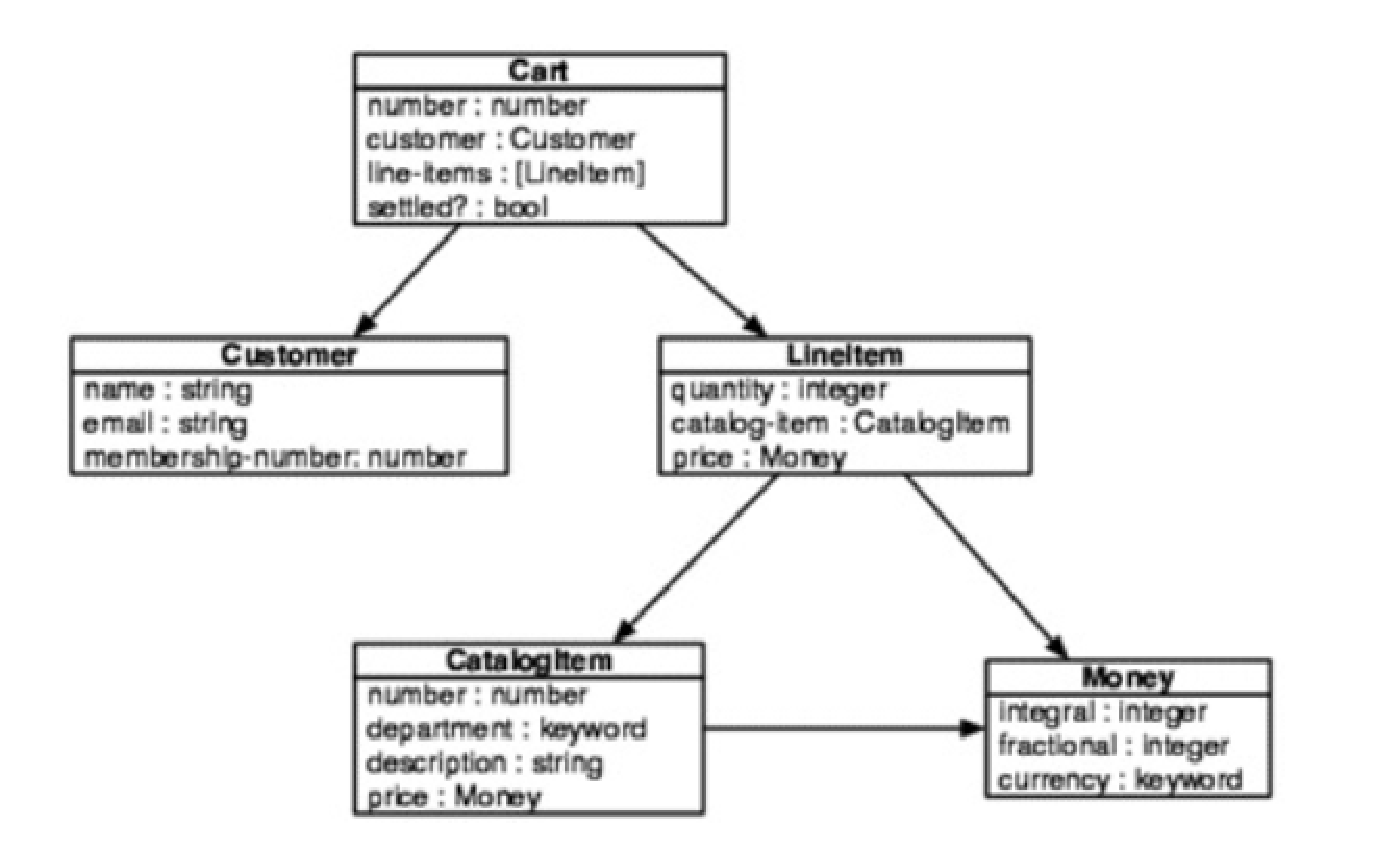
\includegraphics[width=12cm]{fig_03_001.eps}

私たちが求めているのは、もっとシンプルな、部門と金額の対応表です。



\begin{lstlisting}[numbers=none]
{:clothing #Money{:amount 2386424, :currency :usd}
 :toys     #Money{:amount 1163277, :currency :usd}
 ,,, }
\end{lstlisting}

カートの中身から目的の出力まで、順を追って説明しましょう。まず最初にやるべきことは、気になるデータを見つけることです。

\subsection{選択}

シーケンス処理の選択ステップでは、興味のある要素だけを含む部分シーケンスを識別して作成します。カートデータに対してフィルタを使用することで、その要素を取得することができます。

レポートを作成する際、決済されたカートのみを考慮します。決済されるまでは、実際の収益ではなく、潜在的な収益に過ぎないからです。まず、filterを使用してリストのサイズを小さくします。



\begin{lstlisting}[numbers=none]
(defn revenue-by-department [carts]
  (->> (filter :settled? carts)
       ,,,))
\end{lstlisting}

キーワード \texttt{:settled?} を関数として使用すると、 \texttt{:settled?} が\texttt{true}でないカートをすべてフィルタリングすることができます。

\subsection{トランスフォーメーション}

これで一連の決済カートが揃ったので、部門別に収益を分離することができるようになりました。カートは一切必要なく、品目とカタログ品だけが必要なことがわかります。今は一歩ずつ進めていきましょう。次のステップは、すべてのラインアイテムのシーケンスを作成することです。


\begin{lstlisting}[numbers=none]
(defn revenue-by-department [carts]
  (->> (filter :settled? carts)
       (mapcat :line-items)
       ,,,))
\end{lstlisting}

\texttt{(mapcat :line-items ,,)} の結果は、このようになります。


\begin{lstlisting}[numbers=none]
[#LineItem{:quantity 3,
           :catalog-item #CatalogItem{:number   664,
                                      :dept  :clothing,
                                      :desc "polo shirt L",
                                      :price #Money{:amount 2515
                                                    :currency :usd}},
           :price #Money{:amount   7545
                         :currency :usd}},
 #LineItem{:quantity 1,
           :catalog-item #CatalogItem{:number 621,
                                      :dept :clothing,
                                      :desc "khaki pants",
                                      :price #Money{:amount 3500
                                                    :currency :usd}},
           :price #Money{:amount   3500
                         :currency :usd}}, ,,, ]
\end{lstlisting}

\texttt{mapcat}関数は、行項目ベクターの内容を集積したものを構築する。

\begin{itembox}[l]{mapcatとmap + flattenの使い分け}
\texttt{mapcat}の代わりに、\texttt{map}と\texttt{flatten}を併用することで、同様の結果を得ることができます。\texttt{flatten}を使いたくなったら、一歩戻って、そもそも\texttt{flatten}する必要がある構造を作らないようにしましょう。最も一般的なのは、\texttt{map}ではなく\texttt{mapcat}を使うことです(\texttt{map}と\texttt{concatenate}を行うため)。
\end{itembox}

次のステップは、各ラインアイテムから、カタログアイテムの :dept 値とラインアイテムの親の :price 値という気になるデータのマップを抽出することである。これは map と line-summary ヘルパー関数によって行われます。
 % Putting It All Together
% \section{まとめ}

ClojureコレクションはClojureデータの不変のベースを提供し、シーケンスはコレクションと他の順次トラバース可能なデータソースの両方の上に重要な抽象化を提供します。シーケンス関数とトランスデューサの両方を使ったシーケンシャルデータの最も一般的な処理方法を示しました。

トランスデューサーは、シーケンス処理モデルを、ソースの反復処理、変換、出力処理に分割し、それぞれを独立して変更できるようにすることで、より良いパフォーマンスとより多くの再利用性を獲得しています。入力ソースにトランスデューサを適用する3つの一般的な方法として、\texttt{sequence}、\texttt{into}、\texttt{transduce}の使い方を見ました。今後の章では、これらと同じトランスデューサー関数を \texttt{core.async} チャンネルに適用する方法も紹介します。

さて、ドメインをモデル化し、ドメインエンティティをコレクションにグループ化し、それらを処理したところで、スレッドと時間をまたぐ状態の連携を開始する方法を検討する必要があります。 % Wrapping Up


    
         
         
    
    


\part{応用例}

Clojureの状態モデルは、不変のデータと更新関数の基礎の上に構築されています。この状態モデルは、Clojureの参照型の基礎を形成します。状態を安全に共有する方法があれば、同時並行プログラミングは安全で、効率的で、簡単になります。

Clojureコンポーネントは、データ、変換、状態、および並行性を、より大きなコード単位にパッケージ化します。これらのユニットは、アプリケーションに組み入れることができます。


\chapter{状態、アイデンティティ、変化}

あなたは、エンティティ、データのコレクション、ドメイン関数、およびシーケンシャルなデータを処理するためのいくつかの便利なパターンを手に入れました。そろそろ、アプリケーションの実行中におけるドメインデータの連続性について考え始める時期です。

つまり、ドメインエンティティのIDと状態、そしてドメイン内のIDがどのように関連しているかを考える必要があるのです。ドメイン内で一貫した状態管理を行うことで、第5章「コアの使用」で検討する並行処理のためのアプリケーションを準備することができます。

この章では、ドメイン内のエンティティの状態の変更を管理するためのClojureのツールの適用を学びます。より基本的には、アイデンティティと状態を別々のものとして見ていきます。Clojureは、コンピューティング世界のマルチコア状態を利用するように設計されています。状態管理の戦略を選択するための実用的なアドバイスを見つけ、マルチスレッドプログラムを考慮して、ミュータビリティがもたらす落とし穴のいくつかを認識することを学びます。

Clojureアプリケーションのコンテキストで状態とIDが何を意味するのか、その概要から始めましょう。


\section{変更のモデル化}

Clojureの焦点はimmutableな値であることを思い出してください。不変のデータでは、"更新 "は、その場のエンティティまたはエンティティを更新するのではなく、エンティティ(またはエンティティのコレクション)の新しいインスタンスを生成します。ほとんどの場合、この方法で十分に目的を果たすことができます。時には、アプリケーションの世界の変化をモデル化し、データの変化を追跡する必要があります。具体的には、変更されたデータのセットへの参照を保持する必要があります。

マルチスレッドのシナリオでは、その場でデータを更新することは、多くの複雑な問題を引き起こします。誰がデータを変更できるのか?他のスレッドにはどのように変更が通知されるのか?複数の更新が同時に発生した場合、どのプロセスが優先されるのか?Clojureは、状態管理ツールによって、これらの質問すべてにエレガントな答えを提供します。これらのツールを効果的に使用するには、まずClojureのアイデンティティと状態へのアプローチを理解する必要があります。

\subsection{スナップショットで見る}

その理解を助けるために、少し時間の話をしましょう。人間の経験は連続的に見えますが、あなたの感覚は情報を個別の量子に分けて収集しています。音、景色、匂いは、それぞれ独立して脳に入り、時間的な瞬間に相関します。その瞬間が連続して再生されることで、連続した知覚が得られると錯覚しているのです。

もし、自分の視覚的な量子を見るなら、次の図に示すエドワード・マイブリッジの「疾走するサリー・ガードナー」のようなスナップショットの連続が見えるだろう。

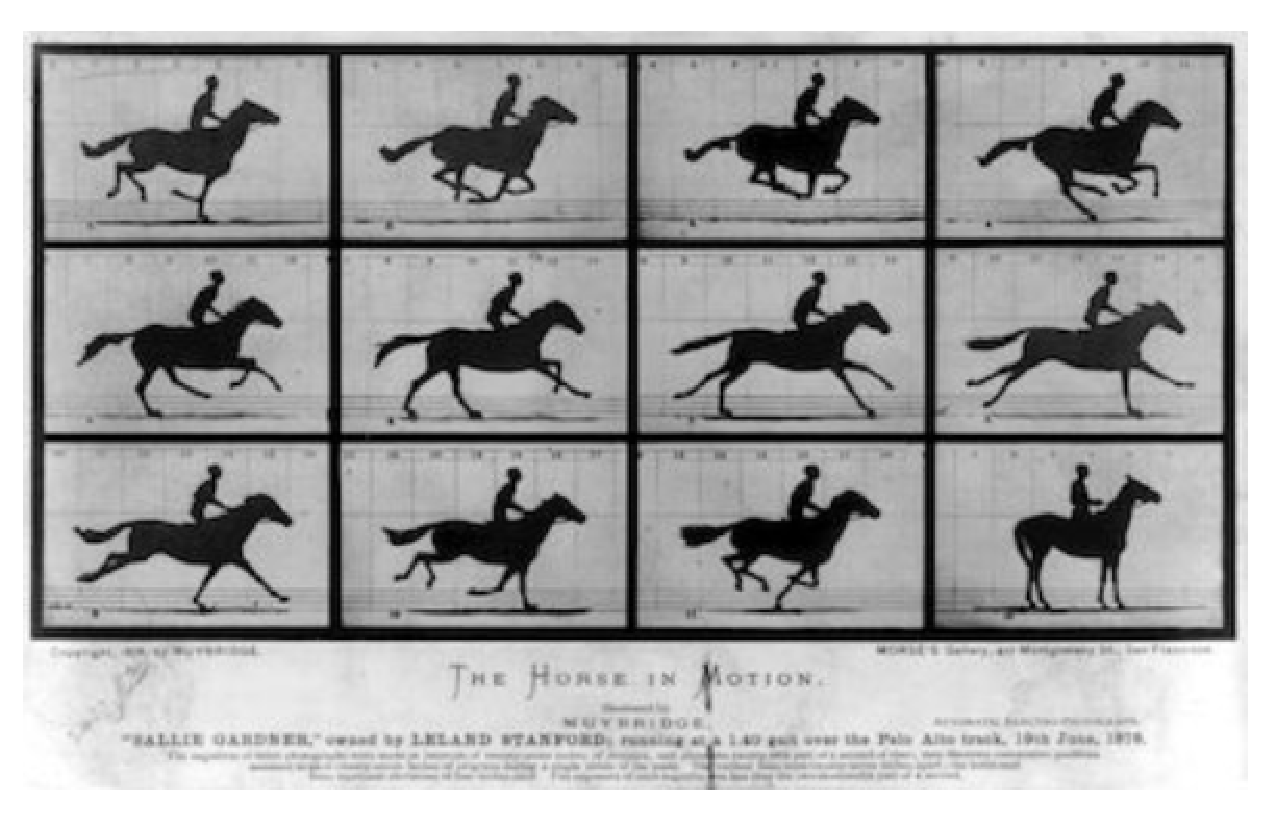
\includegraphics[width=10cm]{fig_04_001.eps}



 % Modeling a Change
\section{変更を管理するためのツール}

Clojureには、アプリケーションの状態を保存するために使用できる4つの参照型(\texttt{var}、\texttt{atom}、\texttt{agent}、\texttt{ref})があります。どの場合にも、メカニズムは、不変の値を格納するミュータブルコンテナを提供します。コンテナは初期値で作成し、その値をリセットすることができます。また、統一更新モデルを用いて状態を進めることもできる。このようにして、アプリケーションの状態を管理された方法で変更することができる。

Clojureの参照型は\texttt{IRef}を実装しています。次の表は、これらの型と、それらの作成、更新、およびリセット関数の一覧です。

\begin{tabular}{|l|l|l|l|}
\hline
IRef & create-fn & update-fn(s) & set-fn \\ \hline \hline
Atom & atom & swap! & reset! \\ \hline
Ref & ref & alter, commute & ref-set \\ \hline
Var & def & alter-var-root & var-set \\ \hline
Agent & agent & send, send-off & restart-agent \\ \hline
\end{tabular}

これらのリファレンスタイプはどれも似たようなパターンです。


\begin{lstlisting}[numbers=none]
;; 作成
(create-fn container)
;; 更新
(update-fn container data-fn & args)
;; 値を設定する
(set-fn container new-val)
\end{lstlisting}

エージェントの場合、作成時にエラー処理オプションを含めることができます。

\texttt{var} はローカルメモリに変更可能なデータを保存し、管理されません。\texttt{atom}は、同期変換(\texttt{swap!}を使用)により保存された値の変更を制限しますが、これらの変更を調整することはありません。\texttt{Ref}は、STMによって、保存された値の制御された変換を提供します。\texttt{agent}は個々のアプリケーションの状態を保存するが、非同期で更新する。(このセクションでは、\texttt{atom}、\texttt{ref}、および \texttt{var} の概要と、それらの使用方法を示す例について説明します。

まず、\texttt{atom}や\texttt{ref}を使用した変更の管理に注目しましょう。


\subsection{Atomによるマネージドアップデート}

データが複数のスレッドによって観測され始めると、それらのスレッドを、調整されていない部分的な更新の混乱から守ることが必要になります。これを怠ると、システムが無効な状態に陥る可能性がある。



\subsubsection{買い物に行こう}

アクティビティをどのようにコーディネートするのがベストなのか、思考を巡らせてみましょう。同時進行の実装を決定するたびに、どの情報を管理し、どの情報を管理しないようにするかを決めるために、同様の演習を行うことになります。

練習のために、食料品の買い物に出かけましょう。まず、シングルスレッドで買い物をすることを考え、次にそのニーズを基に、より複雑なマルチスレッドの例を考えてみましょう。続けて、有用なものができるまで、様々なトランザクションメモリメカニズムを追加していきます。

\subsubsection{ソロオペレーター}

私たちは、食料品の買い物がどのように行われるかを知っています。リストを作り、店に行き、リストにあるものを買うのです。一人の場合、これはとても簡単なことです。リストを作った人が買い物に向かいます。


\begin{lstlisting}[numbers=none]
(defn go-shopping-naive
  "購入した商品の一覧を返します。"
  [shopping-list]
  (loop [[item & items] shopping-list
         cart []]
    (if item
       (recur items (conj cart item))
       cart)))
\end{lstlisting}


このシナリオでは、状態管理は必要ない。1つのスレッド(人)がリストをたどり、おいしいジャンクフードでいっぱいのカートを返します。少なくとも、あなたが大学生の時はそうでしたね。

この例では、すべてが無限の棚に置かれています。私たちは単に、あるリストから別のリストへ物を移動しているだけです。もっと完全な表現にすると、店の在庫を表すことになり、大学生は寮の友達が先にすべてのピザを手に入れたことを発見するかもしれません。その在庫を管理できるようなAPIを書いてみよう。

\subsubsection{ストアAPIの構築}

私たちの店の在庫を、商品と数量のマップとして表現する。複数のスレッドがこの在庫を操作することが予想されるので、どのオブザーバーも一貫したデータを見ることができるようにする必要があります。これは\texttt{atom}で実装することができます。

\texttt{atom}は同期された構造体です。つまり、\texttt{atom}を使用することで、\texttt{atom}に加えたすべての変更が、次の変更が適用される前に完全に行われることを保証します。また、\texttt{atom}は独立であり、非協調でもあります。調整については、次のセクションでもう少し詳しく説明します。最後に、\texttt{atom}はすぐに更新されます。ストアに加え、\texttt{grab}関数と\texttt{stock}関数を定義して、我々の新生APIを形づくることにしよう。


\begin{lstlisting}[numbers=none]
(ns shopping.store)

(def inventory (atom {}))

(defn no-negative-values?
  "マップの値が負であるかどうかをチェックする"
  [m]
  (not-any? neg? (vals m)))

(defn in-stock?
  "在庫を確認する"
  [item]
  (let [cnt (item @inventory)]
    (and (pos? cnt))))

(defn init
"在庫を持つ店舗を構える。"
[items]
(set-validator! inventory no-negative-values?)
(swap! inventory items))

(defn grab
  "棚から品物を取ってくる。"
  [item]
  (if (in-stock? item)
    (swap! inventory update-in [item] dec)))

(defn stock
  "棚に商品を仕入れる"
  [item]
  (swap! inventory update-in [item] inc))
\end{lstlisting}

\texttt{atom}関数を用いて、インベントリがアトムであることを宣言し、その値の変更は、その変更を管理できる関数に限定されることを宣言している。これらの関数は \texttt{swap!}、\texttt{reset!}、さらに低いレベルでは \texttt{compare-and-set!}

インベントリの値はアトム内に格納されているので、値を見るには \texttt{(deref inventory)} または \texttt{@inventory} で参照する必要があります。アトムの値を変更するとき、Clojureは隠れて次のようなことをします。


\begin{enumerate}
\item 現在値をデリファレンス(保存)する
\item \texttt{swap!}に渡された関数を呼び出す.
\item 新しい値を検証するか、例外をスローする
\end{enumerate}

\begin{enumerate}
\item 比較検討する。

\begin{itemize}
\item 参照の現在値が(例えば他のスレッドによって)変更されていない場合、関数の呼び出し結果で置き換え、新しい値を返す。

\item 現在の値がメソッド呼び出し中に変更された場合は、値を置き換えず、最初からやり直します。
\end{itemize}
\end{enumerate}


\subsubsection{無効な状態に対する保護}

\texttt{swap!}メソッドは任務が完了するまで繰り返されます。データの完全なスナップショットに対して関数を呼び出すことが保証されています。しかし、\texttt{swap!}が呼び出されたときにアトムが持っていた値に対して関数を呼び出すことは保証されていない。16行目で定義したバリデータがなければ、負の\texttt{:bacon}が生成される可能性がありますし、誰もそれを望んでいません。このような不運なタイミングの例を見てみましょう。


\begin{lstlisting}[numbers=none]
(:bacon @inventory)                          ;=>1
(if (in-stock? item)                         ; thread 1
(if (in-stock? item)                         ; thread 2
    (swap! inventory update-in [item] dec))) ; thread 2
    (swap! inventory update-in [item] dec))) ; thread 1
(:bacon @inventory)                          ;=>-1
\end{lstlisting}

このように、ガードのタイミングが重要なのです。在庫がマイナスにならないようにするために、19行目でバリデータ関数を渡して保険をかける必要があります。バリデータを使うことで、在庫アイテムの持つ最小値が0であることを保証できます。

アトムの値が変更される前に、新しい値の候補がバリデータ関数に渡されます。バリデータ関数が \texttt{false} を返した場合、アトムを変更しようとすると \texttt{IllegalStateException} がスローされます。バリデータ関数は独自の例外をスローすることも可能で、 その場合は \texttt{IllegalStateException} の代わりとなります。これが可能な場合 (たとえば、\texttt{store.clj} の 22 行目から \texttt{grab} 関数を呼び出す場合)、その可能性に対処する必要があります。一般に、バリデータは単一の引数を取る副作用のない関数 (または \texttt{nil}) でなければなりません。この関数は何度も呼び出すことができることを思い出してください。

(インベントリを定義するときにバリデータ関数を宣言することも簡単にできます。


\begin{lstlisting}[numbers=none]
(def inventory (atom {} :validator no-negative-values?))
\end{lstlisting}

これは、特に初期状態を渡す場合に便利です。バリデータはアトム生成時に初期状態を検証します)。

さて、エマージェント・ストアAPIを使い、ループを\texttt{reduce}に置き換えることで、よりすっきりしたアプローチになりました。このコードは\texttt{go-shopping-naive}関数を置き換えます。


\begin{lstlisting}[numbers=none]
(defn shop-for-item [cart item]
  "商品を購入し、カートを更新して戻る。"
  (if (store/grab item)
    (conj cart item)
    cart))

(defn go-shopping
  "購入した商品の一覧を返します。"
  [shopping-list]
  (reduce shop-for-item [] shopping-list))
\end{lstlisting}

このシンプルな例でも、いくつかの熟考されたステップを経て、APIが形作られ始めていることに注目してください。このようなことは、いつでもどこでも起こっているはずです。考えて、実行して、小さな驚きが生まれるのです。


\subsection{在庫を見る}

毎週毎週、大学生にラーメンを食べさせるためには、お店は定期的に補充をしなければなりません。マスターリストや設定ファイルから定期的に補充することも可能ですが、その場合、スケジュールを気にする必要があります。そこで、「見る(ウォッチ)」機能を追加することを検討してみてはどうだろう。

ウォッチは、物事を監視するために存在します。これは、オブジェクト指向言語におけるObserverデザインパターンの実装に相当するもので、ほとんど同じ目的を果たす。しかし、ウォッチにはほとんどオーバーヘッドがありません。Clojureはウォッチの登録と通知を処理するので、ウォッチャー関数は単純な関数のままです-具体的には、キー、ウォッチへの参照、古い値、新しい値という4つの引数からなる関数です。

ウォッチ機能は、すべての参照型に適用できる。一つの参照に複数のウォッチャーを持つことができ、それぞれが異なるキーを持ち、参照される値が変更されると、すべてのウォッチャーが更新されます。

例を挙げましょう。例えば、ある商品が在庫からなくなったときに、店に通知するためにウォッチ関数を使用するとします。


\begin{lstlisting}[]
(declare sold-items)

(defn restock-order
  "再入荷ウォッチ"
  [k r ov nv]
  (doseq [item (for [kw (keys ov)
                     :when (not= (kw ov) (kw nv))] kw)]
    (swap! sold-items update-in [item] (fnil inc 0))
    (println "need to restock" item)))

(defn init-with-restock
  "店舗を構え、在庫を持つ"
  [m]
  (def inventory (atom m))
  (def sold-items (atom {}))
  (set-validator! inventory no-negative-values?)
  (add-watch inventory :restock restock-order))
\end{lstlisting}

イニシャライザーを変更し、17行目にウォッチ関数を追加しています。ウォッチ関数は次のような形式をとります。

\begin{lstlisting}[numbers=none]
(defn watch-fn [watch-key reference old-value new-value] ,,,)
\end{lstlisting}

このメソッドは、アトムの値が正常に更新されるたびに呼び出されます。古いインベントリ値と新しいインベントリ値を比較し、変更されたアイテムを新しいアトムである\texttt{sold-items}に抽出します。\texttt{grab}は一度に1つのアイテムしか取り出さないことが分かっているので、単純なインクリメントで満足できます。

ウォッチ関数は4つのパラメータを取ります。関数のキー、ウォッチされる参照、古い値、新しい値です。最後の3つは簡単ですが、キー(例えば\texttt{:restock})は不透明な場合があります。裏を返せば、このキーはリファレンスに付けられたウォッチ関数のハッシュマップの中でウォッチ関数を特定するものです(\texttt{.getWatches}関数で取得可能)。このキーは \texttt{remove-watch} でウォッチ関数を削除したり、\texttt{add-watch} で既存のウォッチ関数を置き換えたりするのに使用されます。一般に、キーはラベルとして扱うことができ、あまり気にする必要はありません。

これで、棚から商品が取り出されたことを検出できるようになったので、棚を補充してみましょう。

\subsection{棚の再入荷}

売れた商品を記録するようになったら、定期的に棚を補充したくなるかもしれません。ここでは、かなり地味な補充方法を実装することにする。在庫と売れた商品の両方をリセットします。



\begin{lstlisting}[numbers=none]
(defn restock-all
  "restock all items sold" 3 []
  (swap! inventory #(merge-with + % @sold-items))
  (reset! sold-items {}))
  ; be careful, here be dragons.
\end{lstlisting}

でも、ちょっと待ってください! このようにシンプルにしすぎたために、いくつかの重要なことを見逃しています。ストアのAPIを使うと、それがすぐにわかります。


\begin{lstlisting}[numbers=none]
user=> (use ['shopping.store :as 'store])
nil
user=> (store/init-with-restock {:apples 1 :bacon 3 :milk 2})
#<Atom@eb74118: {:bacon 3, :apples 1, :milk 2}>
user=> (store/grab :bacon)
need to restock :bacon
user=> (store/grab :bacon)
need to restock :bacon
{:bacon 1, :apples 1, :milk 2}
user=> (store/grab :milk)
need to restock :milk
{:bacon 1, :apples 1, :milk 1}
user=> @store/sold-items
{:milk 1, :bacon 2}
user=> @store/inventory
{:bacon 1, :apples 1, :milk 1}
user=> (store/restock-all)
need to restock :bacon
need to restock :milk
\end{lstlisting}

先ほどのセッションで出力された最後の2行は、私たちの見落としの一つを示すものです。\texttt{restock-all}の中で\texttt{swap!}を使って在庫を更新したとき、ウォッチ関数が呼び出され、売れた商品のリストに新しい項目が2つできました。なぜ、3つではなく2つなのでしょうか?なぜなら、ウォッチ関数は数量の変化を調べるようには設計されておらず、売れた商品の名前だけを記録するように設計されていたからです。同じことが、stockを呼び出した場合にも起こります。

もうひとつの見落としは、もう少し曖昧なままです。私たちは、この世界を同時並行的に理解しようとしていることを思い出してください。\texttt{restock-all}関数では、5行目の直前にカオスが入り込む隙間ができています。もし他のスレッドがその時にインベントリからアイテムを取ってきたら、\texttt{sold-items}アトム内のそのアイテムのエントリは消去され、次に再入荷する時にアイテムが不足することになります。

この場合、インベントリ・コンテナのアトム選びは失敗したことになる。この実装では、在庫は独立して同期的に追跡されることを意図していた。しかし、2つ目のアイテム追跡機構を追加すると、突然、物事を調整する必要が生じます。たとえ少数のものでも調整するのは難しい。このトリッキーさには \texttt{refs} を使って対処できます。

\subsection{Refによるトランザクションの変更}

より複雑なドメインでは、複数の値の同時更新を調整する必要があるため、アトムはもはや機能しません。トランザクションの力が必要であり、それには一連の参照関数が必要である。これを複雑な買い物の例で示そう。


\subsubsection{パックでお買い物}


お子さんがいらっしゃる方は、お子さんを連れてきてカートに入れるのを手伝ってもらうといいかもしれませんね。この場合、ある程度の連携が必要になるので、どのようなやり方が最適かを決める必要があります。

簡単なシナリオとしては、買い物リストを子どもたちに分担させ、各自のリストにある商品を取りに行かせます。買い物を終えた子どもたちが戻ってきたら、最後に商品を組み合わせます。

これで問題解決ですね。役割分担をすることで、コーディネートの問題を先に解決し、その後の協力は不要になったのです。状態管理:回避

もちろん、これは子供たち全員が同じ注意力を持っていて、リストにあるものを見つけるためにベストを尽くし、気が散らないようにし、他のものを持ち帰らないことを前提としています。もしこれがすべて真実であれば、物事は順調に進むと期待できます。子供の買い物へのアプローチをより現実的に実行すると、次のようになります。



\begin{lstlisting}[numbers=none]
(defn dawdle
  "ぶらぶらしたり、迷子になったり、お菓子を買ったり"
  []
  (let [t (rand-int 5000)]
    (Thread/sleep t)
    (maybe? buy-candy)
    ))
\end{lstlisting}

ちょっとしたカオスが加わったので、それを緩和する必要があります。子どもたちを1つずつ探しに行かせ、ある程度の時間、ぐずぐずさせます。戻ってきたら、その商品とお菓子をカートに入れ、次の課題を受け取ります。集中力のある子供たちは、より多くの仕事をこなしますが、アイテムは最終的にリストから取り除かれます。

\subsubsection{ルールからトランザクションを構築する}

ここでの成功の鍵は、買い物をする商品に関する明確なルールを持つことです。そのルールがあれば、そのルールに従ったモデル化と状態の更新を行いたい。

ルールは簡単だ。

\begin{itemize}
\item 買い物リストのアイテムは、子供に割り当てられると消去される。

\item カートに入れるまで、その商品は子供に割り当てられたままです。

\item お菓子は買い物リストにもカートにも入れられません。
\end{itemize}

我々のルールを守るために、ローカルな世界から見て、子供に品物を割り当てることと、買い物リストから取り除くことは同時に行われなければなりません。同様に、商品を回収することと、カートに入れることも、事実上同時に行わなければならない。これらの動作を調整するために、1つまたは3つの参照が必要です。

\texttt{ref} はその値を \texttt{ref world} に保存し、その値への変更がトランザクションとして協調的かつ同期的に実行されることを保証するのに役立ちます。次の例では、3つの\texttt{ref}を作成しています。\texttt{shopping-list}は買い物をする予定のアイテムを保持するセットである.子供の名前をマップキーとして、割り当てマップで飛行中のアイテムを追跡する。最後に、ショッピングカートは、子供から回収したアイテムのセットである。


\begin{lstlisting}[numbers=none]
(def shopping-list (ref #{}))
(def assignments (ref {}))
(def shopping-cart (ref #{}))

(defn init []
  (store/init {:eggs 2 :bacon 3 :apples 3
               :candy 5 :soda 2 :milk 1
               :bread 3 :carrots 1 :potatoes 1
               :cheese 3})
  (dosync
    (ref-set shopping-list #{:milk :butter :bacon :eggs
                             :carrots :potatoes :cheese :apples})
    (ref-set assignments {})
    (ref-set shopping-cart #{})))
\end{lstlisting}

\texttt{ref}の値の変更は、\texttt{dosync}を使用して、トランザクションの内部で行わなければなりません。トランザクションは多くの更新で構成されます。

これらの更新には3つの種類があります。\texttt{ref}の値を直接更新する場合、\texttt{ref-set}を使用します。関数を使用して更新する場合は、\texttt{alter} または \texttt{commute} を使用します。最も頻繁に見るのは、再初期化のコンテキストで \texttt{ref-set} を見ることでしょう。

\texttt{alter}を使用する場合、関数を適用したときの\texttt{ref}の値が、トランザクションの開始時、または現在のトランザクション内で最後に\texttt{alter}関数が適用されたときの\texttt{ref}の値と同じであることが必要です。このトランザクションの実行中に、同時に実行されているトランザクションによって \texttt{ref} が更新された場合、再試行のトリガとなります。トランザクションが外部からの干渉を受けずに実行される必要がある場合、\texttt{alter} 関数は使用すべき関数です。

トランザクションが内部一貫性のチェックを必要としない場合、\texttt{commute}を使用することができます。\texttt{commute}関数は、トランザクションの実行中に\texttt{ref}の値が変更されても、再試行の引き金にはなりません。\texttt{commute}に渡された関数は、\texttt{ref}がその時点で持っているどのような値に対しても実行されます。

同時実行性の高いアプリケーションでは、可能な限り \texttt{alter} 呼び出しを \texttt{commute} に置き換えることで、再試行を回避して性能を向上させることができます。これは、\texttt{commute} に渡される関数が可換である場合、つまり、更新関数を適用した結果が実行順序に関係なく同じ結果になる場合にのみ実行されるべきです。足し算を考えてみてください。(4 + 6 + 2)は(2 + 4 + 6)と同じになります。

\texttt{ensure}関数は、\texttt{ref}の値が更新されずに現在のトランザクションの外で変更されていないことを確認するために使用することができます。値が変更されたことを確認した場合、再試行を開始します。これは、\texttt{ref} が相互に依存した値を持つような状況で有用です。例えば、購入を完了するとき、価格を更新していないにもかかわらず、トランザクション中に価格が変更されていないことを確認するために、価格リスト上で\texttt{secure}を行うかもしれません。トランザクションの途中で価格が変更された場合、再試行が行われるはずです。

\texttt{ref} の更新の構文を簡単に説明すると、更新を行う関数と引数を送信することで \texttt{ref} を変更(またはコミット)します。

次のコードブロックでは、トランザクションを実行するために必要な関数を定義しています。もう一度言いますが、このコードからAPIが生まれ始めているのがわかります。\texttt{assign-item-to-child} 関数は、ショッピングリストからアイテムを削除し、それを子に割り当てます。\texttt{collect-assignment}関数は、ショッピング・カートに買い物した商品を追加し、子プロセスの割り当てを破棄します。先ほどの\texttt{dawdle}関数は\texttt{buy-candy}を使用しています。以下はトランザクションです。


\begin{lstlisting}[numbers=none]
(defn assignment
  [child]
  (get @assignments child))

(defn buy-candy []
  (dosync
    (commute shopping-cart conj (store/grab :candy))))

(defn collect-assignment
  [child]
  (let [item (assignment child)]
    (dosync
      (alter shopping-cart conj item)
      (alter assignments dissoc child)
      (ensure shopping-list) ;; not needed
                             ;; included as an example
      )
    item))

(defn assign-item-to-child [child]
  (let [item (first @shopping-list)]
    (dosync
      (alter assignments assoc child item)
      (alter shopping-list disj item))
    item))
\end{lstlisting}

前述のメソッドはいずれも、ローカル制御が戻る前に完全に更新する必要がある、状態の2つの異なる要素に対して操作します。これらのメソッドは、\texttt{alter} を使用して、変更されるコレクションを更新し、操作がこの順序で実行されることを示します。また、更新されなかった参照を保護するために \texttt{ensure} を使用します。

トランザクション(\texttt{dosync})が実行されている間、\texttt{dosync}ブロックで特定された参照への書き込みは防止されます。これらの変更はすべて提案され、次に代替タイムラインである \texttt{ref} の世界にコミットされます。すべてが正常に終了した場合、すべての更新は書き込みポイントの後にローカルワールドで読むことができるようになります。そうでなければ、変更はコミットされず、トランザクションは再試行回数制限(この記事の執筆時点では10,000回)に達するまで再試行されます。これにより、実行中のすべてのスレッドで我々のルールが維持されることが保証されます。


\subsubsection{買い物に行く}

さて、トランザクションメソッドの定義ができたので、実際に買い物に行くことができます。


\begin{lstlisting}[numbers=none]
(defn send-child-for-item
  "eventually shop for an item"
  [child item q]
  (println child "is searching for" item)
  (dawdle)
  (collect-assignment child)
  (>!! q child))

(defn report []
  (println "store inventory" @store/inventory)
  (println "shopping-list" @shopping-list)
  (println "assignments" @assignments)
  (println "shopping-cart" @shopping-cart))

(defn go-shopping []
  (init)
  (report)
  (let [kids (chan 10)]
    (doseq [k my-kids]
      (>!! kids k))
    (go-loop [kid (<! kids)]
      (if (seq @shopping-list)
      (do
        (go
          (send-child-for-item kid (assign-item-to-child kid) kids))
        (recur (<! kids)))
      (do
        (println "done shopping.")
        (report))))))
\end{lstlisting}

\texttt{go-loop}や奇妙なエイリアンのアルファベット(\texttt{<!}, \texttt{>!})に見覚えがあっても心配しないでください。これらは\texttt{core.async}の一部で、第5章「コアの使用」で並行処理について説明するときに詳しく説明します。今のところ、ループを開始するときにキューから子オブジェクトを取得し(チャネルと呼ばれます)、その子オブジェクトに割り当てられたアイテムを収集した後にキューに戻すということを知っておいてください。

それ以外は、買い物そのものはかなり直感的に進められる。トランザクションをできるだけシンプルに、できるだけ少ない場所で行うことで、カオスになるリスクの多くを軽減しています。

そういえば、お菓子の話はしていませんでしたね。ルールではお菓子はダメなので、バリデーターをショッピングカートに追加しましょう。


\begin{lstlisting}[numbers=none]
(def shopping-cart (ref #{}
  :validator #(not (contains? % :candy))))
\end{lstlisting}

また、どうしてもお菓子が入ってしまったときにカートを爆発させたくなければ、それが起きたときに親に通知する監視機能を追加して、罰に関する判断を遅らせることもできます。


\begin{lstlisting}[numbers=none]
(defn notify-parent
  [k r _ nv]
  (if (contains? nv :candy)
    (println "there's candy in the cart!")))
\end{lstlisting}

ウォッチ機能を作成したら、initでショッピングカートに追加します。


\begin{lstlisting}[numbers=none]
(add-watch shopping-cart :candy notify-parent)
\end{lstlisting}

最後に、varコンテナについて考えてみましょう。





\subsubsection{Varでローカルな状態を追跡する}

最後に、すべての状態について管理が必要なわけではありません。変更されないデータ(システムの状態など)には変更管理は必要ありません。同様に、他のスレッドから観測されないデータも管理する必要はありません。このような場合、データを保存するためにvarを使用します。\texttt{def}を使って、var を設定する:


\begin{lstlisting}[numbers=none]
user=> (def my-kids #{:alice :bobby :cindi})
\end{lstlisting}

このvarは、現在の名前空間内のシンボル(\texttt{my-kids})を持つグローバルなスコープを持つ。もしその var がすでに存在すれば、新しい値が設定される。この var は好きなように読み込んで再定義することができます。\texttt{alter-var-root} を使って、var を更新します。\texttt{my-kids} の前の \texttt{\#'} に注意してください: \texttt{alter-var-root} には、その値ではなく、var 自体を渡します。


\begin{lstlisting}[numbers=none]
user=> (defn born! [new-kid] (alter-var-root #'my-kids conj new-kid))
#'user/born!
user=> (born! :donnie)
#{:donnie :alice :bobby :cindi}
\end{lstlisting}

グローバルな定義を損なうことなく、ローカルバインディングやスレッドでvarを再定義できるようにしたい場合、定義時にこの効果を持たせるためのメタデータを追加することが可能です。


\begin{lstlisting}[numbers=none]
user=> (def ^:dynamic my-kids #{:alice :bobby :cindi})
#'user/my-kids
user=> (print my-kids)
#{:alice :bobby :cindi}
user=> (binding [my-kids #{:luke :leia}]
#_=>     (print my-kids))
#{:leia :luke}
user=> (print my-kids)
#{:alice :bobby :cindi}
\end{lstlisting}

Varsはステートフルですが、ローカルメモリに保存されるため、管理されることはありません。var に動的スコープを追加すると、そのバインディングはローカライズされますが、別の問題が発生します。Stuart Sierra はこの問題について "On the Perils of Dynamic Scope" という記事を書いています[18] 要するに、本当にそう思っていて、自分が何をしているのか分かっていない限り、この方法はとらない方がいいということです。

我々は、Clojureがrefとatomとそれらに関連する更新関数でアプリケーションの状態の変更を管理するために提供する主要な構造のほとんどを歩いてきました。また、グローバルな状態を保存するための var も簡単にレビューしました。さて、変更を管理するためのツールを手に入れたので、どのように変更と付き合っていくかについて少し話をしましょう。

次のセクションでは、管理された変更に関する適切な実装上の決定を行う方法と、変更可能性の影響を制限しながらAPIを成長させるための2つのアプローチについて学びます。 % Tools for Managing Change
\section{変化と生きる}

Clojureが提供する、アプリケーションの状態を更新するためのツールをいくつか詳しく見てきました。これらのツールは、変更が有効であり、瞬時に見えることを保証することで、不運から守ってくれます。しかし、まだずさんな考えで自分自身の足を撃つことができます。

状態管理の複雑さを、ドキュメントやブログ記事、そしてこの本のようなおもちゃのようなコードで示すことは困難です。しかし、これまで見てきたような仕組みを応用する際には、いくつかのガイドラインを心に留めておくとよいでしょう。

\subsection{バリデーションの方法とタイミング}

私たちの\texttt{shopping.store} APIは、冗長性と少し厄介な部分を含んでいます。\texttt{init}では、私たちのAPI(特に\texttt{grab})を無視してストアの\texttt{inventory}を直接更新するコードから保護するために、バリデータ関数として在庫に\texttt{no-negative-values?}関数を適用しました。

このバリデータメソッドは、マップのすべての要素を検査して、在庫が増加していることを確認します。在庫が大きくなり始めたらどうなるのでしょうか?\texttt{grab}で使っている\texttt{in-stock?}テストと比較して、どれだけのオーバーヘッドになるでしょうか?厄介なことに加えて、冗長です。\texttt{grab}を使おうが使うまいが、バリデータは呼び出されるのです。

どうすればいいでしょうか?少なくとも、\texttt{inventory}の\texttt{def}に \texttt{\^\{:private true\}} を追加して、\texttt{grab} の使用を奨励すべきです。より堅牢な解決策は、システムを初期化する関数を構築し、それを必要とするコンポーネントに渡すことです。これは、第7章「アプリケーションを構成する」で詳しく説明するコンポジションの水域に足を踏み入れることになります。

APIを開発する際には、必要と思われるすべてのアクションをラップした一連の関数を提供し、実際のデータの保存は非公開にするようにしましょう。こうすることで、提供された関数をバイパスして直接データを操作することを防ぐことができます。これにより、バリデータのパフォーマンスが低下するような場面でも、 不正な操作から保護する仕組みを導入することができます。バリデータ関数は Clojure がトランザクションをコミットする前に実行されるので、 長時間実行するバリデータはステートフルなリソースへのリクエストをブロックしたり キューに入れたりする可能性があることを覚えておいてください。

一方、バリデータ関数の定義は、小さなデータやプログラムの状態には効果的です。(たとえば) ロギング用のファイル名を含むアトム設定がある場合、 そのファイルが存在するかどうかをバリデータに確認させたいことがあります。ひとつのアトムでさまざまな更新が可能な場合、バリデータを使用すると検証を一元化でき、 必要なコードの量を減らすことができます。もちろん、誰かがルールを破ったときに発生する例外をキャッチする準備はしておかなければなりませんが、 設計とは常にトレードオフの関係にあるものなのです。

\subsection{ランタイムステートとプログラムステート}

安心してください、これは少しは分ける価値があります。この章では、主にプログラムの状態やアプリケーションの状態について話してきました。つまり、インベントリやショッピングリストなど、問題領域にある管理された状態を対象にしてきました。プログラム状態は、ソフトウェアがモデル化するドメイン知識と、ソフトウェアが解決しようとする問題に直接関連するデータと概念に、管理されたアクセスを提供する役割を果たします。

店舗APIにはinventoryアトムがあり、そこにsold-itemsアトムを後から追加した。家族での買い物は、買い物リスト、割り当て、ショッピングカートを管理した。これらの要素はすべてプログラム・ステートである。プログラムの状態には、可能な限りAPIを使ってアクセスし、直接ではなく、慎重に吟味されたメソッドを通して使用されるべきである。

一方、ランタイムステートは、ソフトウェアの実行を容易にするために存在する。ランタイム状態は、データベース、設定ファイル、ネットワーク接続、または呼び出す予定のコンポーネントへの参照を保持する役割を果たします。これらは動作環境に影響を与えるもので、ドメイン情報には関係ない。ランタイムステートについては、第7章「アプリケーションを構成する」で詳しく説明します。ランタイムステートはしばしば避けられないもので、設定可能性を損なわずに最小化することは困難です。もしソフトウェアが必要とする状態情報の量を削減したいのであれば、代わりにプログラムの状態に注目しましょう。

関数型プログラミングに慣れないうちは、反射的にドメインに不必要なミュータビリティを散りばめてしまいがちです。この傾向は2つの方向から攻めることができます。1つ目は、前もってそれを確認すること、2つ目は、最後に変異性を減らすことです。


\subsection{変化に対応する}

Clojureの核となる原則に忠実であれば、Clojureの力を最大限に引き出すことができます。変更を管理する場合、アプリケーションのニーズを満たすのに十分なものを作りたいものです。これまで概説したプロセスでは、問題領域とそのエンティティおよび変換から、アプリケーション領域、連続性、およびコンポーネント間の相互作用に焦点を移すまで、プログラム状態の開発が自然に制限されます。あなたは、アプリケーションの開発経路において、次のような状態になっているはずです。

あなたは、不変の値であるエンティティを構築しました。それらはステートフルなものには依存せず、自身のドメイン値のみに依存します。複雑なエンティティは、より単純なエンティティを含むことができますが、それでも値でしかありません。

変換は純粋な関数である。値を取り込み、値を吐き出す。コレクションを変換するものは、コレクションを引数として受け取り、新しいコレクションを返します。複数のドメインにまたがる機能を持つようになると、プログラムの状態ではなく、値が取引材料になることが保証されます。

これらのことが解決された後に初めて、プログラム状態が必要になります。トランザクション管理機能を書くのは、早めではなく、遅めになります。管理された変更の必要性は、優れた開発プラクティスによって制限されてきました。しかし今、あなたはアプリケーションレベルの関心事に忍び込んでいます。ドメインの言語と機能をシステムのユーザーにつなげるために、プログラムステートが必要なのです。

アプリケーションの状態は、どの程度が過剰なのか、判断が難しいところです。Refsやvarsなどの数で不正確な抽象的な尺度を考えるよりも、Clojureでソフトウェアを設計するときに次の真実をしっかりと心に留めておいてください:すべての副作用と変更可能な参照はあなたの速度を遅くします。

 % Living with Change
\section{まとめ}

アプリケーションを構築するとき、私たちはしばしば、そうでなければ純粋なアプリケーションを通して更新を進めていくことに気づきます。もし私たちがルールを明確にし、関数に責任を持ち、管理する必要があるものを正しく選択するならば、効果的にそれを行うことができます。

データとその状態の変化を一連のスナップショットとして見ることで、他のプロセスのオブザーバの存在を考慮した上で、責任ある行動をとることができる。Clojureでは、それらのスナップショットは、ミュータブルな参照に包まれた以前のバージョンとして保持されます。これは、すべてのオブザーバーが特定の瞬間の値の一貫したセットを持っていることを保証し、誰も不幸な状況に自分自身を見つけることはありません。

この章では、時間の観点から見たアイデンティティと状態についてのアイデアを探求することから始めました。これらのアイデアを使用して、Clojure の vars によるグローバルな状態、および atoms と refs を使用して更新を管理する機能について学びました。これらのことはすべて、時間の経過とともにストーリーを整理しておくのに役立ちます。これで、並行処理に進むためのツールを手に入れました。

次の章では、並行処理について考えていきます。また、子供と一緒に買い物に行ったときに見た core.async をより深く見ていきます。エージェントは、私たちの管理対象名簿を完成させるでしょう。 % Wrapping Up % State, Identity, and Change



\section{待機をバックグラウンドに押しやる}

ほとんどのプログラムは、ファイル、ソケット、標準的なターミナルストリームを通して外部世界と接続します。これらすべてを入出力、I/Oと呼んでいます。最近のプロセッサは1秒間に何十億もの命令を実行することができますが、ほとんどのI/Oは比較的低速です。多くのプログラムは、ファイルからデータを読み込んだり、外部サーバーから応答を受け取ったり、ユーザーが何をしたいのかを調べるために、かなりの時間をかけて待機しています。

プログラムが他の作業を続けられるように、この待ち時間を効率的に処理する必要があります。待っている間、私たちは他の処理を行うこともできますし、複数の処理を並行して待つこともできます。例えば、ウェブブラウザは、外部のウェブサーバがコンテンツを返すのを待つと同時に、現在のページをレンダリングし、ユーザーがリンクをクリックしたりページをスクロールしたりするのに応答して時間を費やしているプログラムである。

\subsection{ファイヤー・アンド・フォーゲット}

まず、バックグラウンドで応答不要な作業を行うという単純なケースを考えてみよう。アプリケーションを構築しているときに、イベントが発生するたびに外部の計測器コレクターを呼び出したいとします。この外部サービスは、inc-stat という便利な関数でラップすることができます。更新するstatを指定して、この関数を呼び出します。


\begin{lstlisting}[numbers=none]
(inc-stat :pageview)
\end{lstlisting}

この関数は、ネットワーク経由で外部のウェブサービスを呼び出そうとしています。もし、ページビューを制作中に呼び出すと、次の図にあるように、その呼び出しにかかる時間は、ページを構築するごとに遅くなってしまいます。


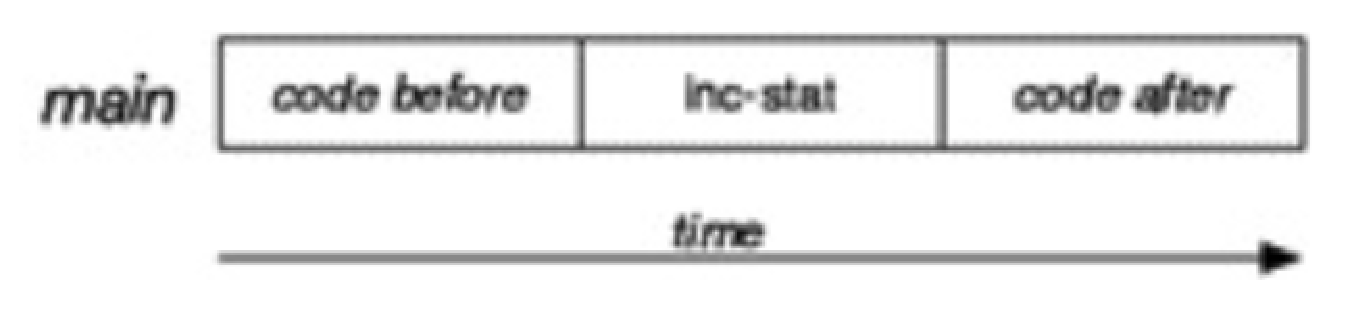
\includegraphics[width=10cm]{fig_05_001.eps}

この作業をバックグラウンドのスレッドに移すために、Clojureに含まれる\texttt{future}関数を使用します。

\begin{lstlisting}[numbers=none]
(future (inc-stat :pageview))
\end{lstlisting}

\texttt{future}関数はボディを受け取り、Clojure自身が維持するバックグラウンドのスレッドプールでそのボディを呼び出す。図にその違いを見ることができます。

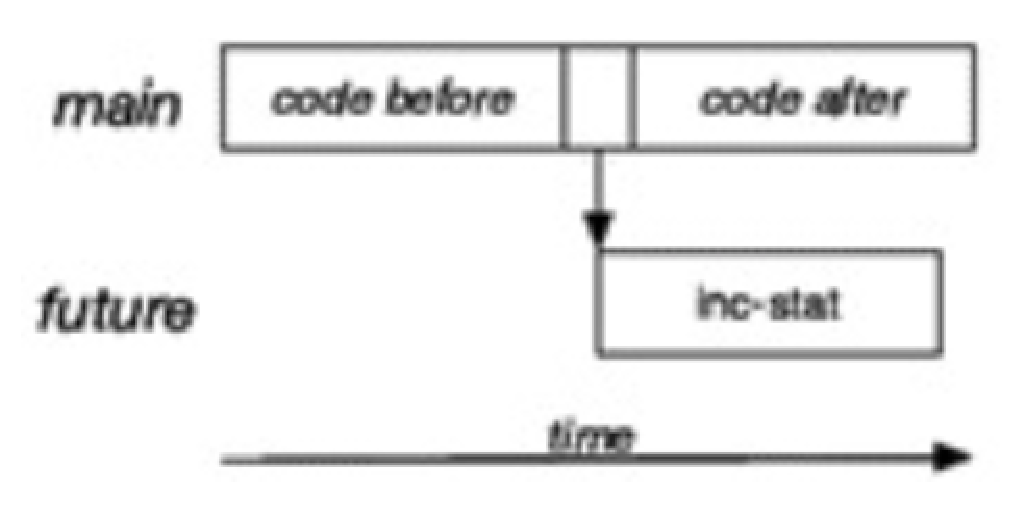
\includegraphics[width=8cm]{fig_05_002.eps}

また、\texttt{future-call}を使用すると、ボディを渡す代わりに引数のない関数を非同期で呼び出すことができます。どちらの関数も\texttt{java.lang.Future}オブジェクトを返し、それを使って非同期の活動を制御したり検査したりすることができます。\texttt{future-cancel}関数はその実行をキャンセルし、\texttt{future-done?}と\texttt{future-cancelled?}はその状態についての情報を与えてくれます。

しかし、独立した統計値増加メッセージをリモートサービスに大量に送信するのは非効率的だと思われます。送信前にいくつかのインクリメントメッセージをバッチ処理する方がより理にかなっています。そのためには、非同期かつステートフルである必要がある。


\subsection{非同期とステートフル}

第4章「状態、アイデンティティ、変化」では、Clojureの状態コンテナであるvar、atom、refを検討しました。もう一つの状態コンテナであるagentの紹介は、今まで遅らせました。

他のステート・コンテナと同様に、agentは不変の値を保持し、同じ更新モデルを使用して変更されます。他のコンテナとは異なり、agentは非同期に更新されます。

メトリクス・コレクターを考えてみましょう。ある統計量のカウンターをagentに保持することにしましょう。

\begin{lstlisting}[numbers=none]
(def pageview-stat (agent 0))
\end{lstlisting}

agentの更新ごとにリモートサービスを呼び出すのではなく、10回目の更新(agentの状態が10で割り切れる回数に達したとき)ごとに呼び出すことにします。これは、ウォッチ(すべてのステートコンテナで動作する)を使えば簡単にできます。


\begin{lstlisting}[numbers=none]
(add-watch
  pageview-stat
  :pageview
  (fn [key agent old new]
    (when (zero? (mod new 10))
      (remote-send key new))))
\end{lstlisting}







 % Push Waiting to the Background
\section{キューとワーカー}

多くのプログラムは、その全体または一部をタスク処理系として見ることができます。タスクとは、通常、外部からの要求に対応する作業の単位です。ウェブアプリケーションは、ウェブページを作成するためのリクエストを受け取ります。ウェブサービスは、APIコールを処理するリクエストを受け取ります。バッチプログラムはディスクやデータベースからファイルを読み込んで、それぞれを適切に処理する。これらの一般的なパターンはすべて、ワーカーのプールに委託された作業のキューとしてモデル化することができます。

キューは、タスクの順序付けと保持を行い、ワークが到着する場所と処理される場所を切り離します。ワーカープールでは、異なる特性を持つワーカーのプールを作成し、並行処理や、作業の管理・監視に使用するポリシーを制御することができます。その制御により、自由に使えるハードウェアをフルに活用することができるのです。

Clojureはキューとワーカーのためのいくつかのツールを提供しますが、Javaですでに利用可能な高品質のツールを再発明することも避けます。Clojureで既に見てきた部分から、キューとワーカープールをどのように作成できるか考えてみましょう。

\subsection{組み立てが必要}

第1章Model Your Domainでは、Clojureの永続キューを使用して、FIFOデータに対してリストやベクターよりも効率的なアクセスを提供しました。しかし、これはシングルスレッドのコンテキストで行われました。永続的なキューでは、キューを変更するたびに、更新されたバージョンが返されます。もし複数のスレッドがキューを共有するならば、それら全てが同じインスタンスを共有する必要があります。そのため、(atom や ref などの) 状態管理構造体か、状態管理型のキュー実装のいずれかが必要になります。

1つのオプションは、キューの両端が安定したアイデンティティを維持するように、Clojureのアトムまたは参照に永続的なキューをラップすることです。アトムでこれを行おうとすると、アトムの\texttt{swap!}関数がアトムの新しい値(私たちの場合はキュー)を返すだけで、ポップした値を返さないことに気づきます。このため、この種のキューからステートフルな方法でアイテムを取り出すことは困難です。

refオプションはより有望に見えます。このように実装できるだろう。


\begin{lstlisting}[numbers=none]
(defn queue
  "新しいステートフルキューの作成"
  []
  (ref clojure.lang.PersistentQueue/EMPTY))

(defn enq
  "qのitemを待ち受ける"
  [q item]
  (dosync
    (alter q conj item)))

(defn deq
  "qからitemを取り出す(なければnil)。"
  [q]
  (dosync
    (let [item (peek @q)]
      (alter q pop)
      item)))
\end{lstlisting}

しかし、このキューはブロックしない! 通常、キューが空でデータの到着を待っているときにコンシューマが \texttt{deq} でブロックすることを望みますが、この実装では \texttt{nil} を返すだけで、コンシューマが繰り返しポーリングすることを要求されます。この理由から、Clojureの永続的なキューは、通常、スレッド間で仕事のキューを管理するための良いツールではありません。

代わりに、キューとワーカーに対するJavaのサポートに注目する必要があります。これは、Javaライブラリが多種多様な動作に対して強力なサポートを持っている分野です。

\subsection{Javaキュー}

キューとワーカーをサポートするJavaクラスのほとんどは、\texttt{java.util.concurrent}パッケージで見つけることができます。Javaは多くのブロッキングキュー実装(すべて\texttt{java.util.concurrent.BlockingQueue}の実装)を提供し、それらはClojureから簡単に使用することができます。

Java のキュー実装の主な違いの1つは、データのバッファリング方法です。例えば、\texttt{LinkedBlockingQueue}はオプションで境界付きバッファを提供し、\texttt{ArrayBlockingQueue}は境界付きバッファを提供し、\texttt{SynchronousQueue}はバッファを全く提供しません。\texttt{LinkedTransferQueue} は、\texttt{SynchronousQueue} のハンドオフ機能と、オプションで制限されたバッファを組み合わせています。

これまで述べてきたすべてのキューは FIFO 順で値を提供しますが、Java は項目を並べ替えるキューも 2 つ提供します。\texttt{PriorityBlockingQueue} は、優先度の高い項目をキューの先頭にバブリングします。\texttt{DelayQueue}は、遅延のあるメッセージを受け取り、遅延の期限が切れたものだけを利用できるようにします。

Bounded buffer queue は、producer が満杯のバッファに遭遇したときに、カスタマイズする機会も提供します。Java のブロッキングキュー API では,ブロッキング,タイムドブロッキング,特別な値の返送,例外の発生が可能です.

\texttt{put} や \texttt{take} などの \texttt{BlockingQueue} メソッドは、通常の Java interop メソッド呼び出しで呼び出すことができます。それでは、いくつかのメッセージをキューにプッシュしてみましょう。

\begin{lstlisting}[numbers=none]
(ns ch5.jqueue
  (:import [java.util.concurrent LinkedBlockingQueue]))

(defn pusher [q n]
  (loop [i 0]
    (when (< i n)
      (.put q i)
      (recur (inc i))))
    (.put q :END))

(defn popper [q]
  (loop [items []]
    (let [item (.take q)]
      (if (= item :END)
          items
          (recur (conj items item))))))

(defn flow [n]
  (let [q (LinkedBlockingQueue.)
        consumer (future (popper q))
        begin (System/currentTimeMillis)
        producer (future (pusher q n))
        received @consumer
        end (System/currentTimeMillis)]
    (println "Received:" (count received) "in"
             (- end begin) "ms")))
\end{lstlisting}

\texttt{pusher}関数は、キューに\texttt{n}個の数値をプッシュし、最後に完了を知らせる\texttt{:END}メッセージを送ります。\texttt{popper}関数は同じキューから\texttt{:END}メッセージを受け取るまでメッセージを引き離します。これらの関数は両方ともバックグラウンドのスレッドプールで実行される \texttt{futures} で実行されます。

しかし、どのスレッドがこれらの\texttt{future}を実行するかは制御できません。Clojureのfutureとagentは非同期実行のための比較的簡単なAPIを提供しますが、監視と制御が多少損なわれます。その代わりに、多くのスレッド上で作業を実行するためのJavaのビルトインサポートを使用することができます。

\subsection{スレッドの作成}

Javaには、スレッドのファクトリー(\texttt{ThreadFactory})と、キューとワーカープールの組み合わせ(\texttt{ExecutorService})を表現するインタフェースが用意されています。

このように、プロセッサ数に応じた大きさの計算スレッドの固定プールを作成することができます。


\begin{lstlisting}[numbers=none]
(import '[java.util.concurrent Executors])

(def processors (.availableProcessors (Runtime/getRuntime)))

(defonce executor (Executors/newFixedThreadPool processors))

(defn submit-task [^Runnable task]
  (.submit executor task))
\end{lstlisting}

Javaでは、\texttt{Runnable}または\texttt{Callable}インタフェースを用いて実行可能なタスクを表現します。役に立つことに、すべてのClojure無引数関数はこれらのインターフェイスを実装しています。タスク(任意のClojure関数)は、呼び出すために\texttt{ExecutorService}に渡すことができます。したがって、リクエストのストリームをタップして、それらを実行のためのタスクとして送信するのは簡単です。

Java 5で追加されたJavaエグゼキュータは、当時一般的だった4~8コアのマシンで粗視化されたタスク並列をサポートするように設計されています。しかし、マシンのコアが増えるにつれ、1つのキューで待つことによる競合が、キューからアイテムを取得するワーカーのボトルネックとなりました。

この問題に対処し、他の計算パターンを利用するために、Java 7 では \texttt{fork/join} という新しいフレームワークが導入されました。\texttt{fork/join} は、より小さな粒度の細かい計算タスク、再帰的な計算、より多くのコアをサポートするように設計され、調整されています。\texttt{fork/join} は多数のワーカーキューを使用し、それらのキューが互いに仕事を「盗む」ことを可能にします。つまり、あるキューがやるべき仕事を使い果たした場合、別のキューの後ろからタスクを取り出し、キュー間の仕事のバランスを自動的に調整します。

\texttt{java.util.concurrent.ForkJoinPool} クラスは、Java のフォーク/ジョイン実装の主要なエントリポイントです。\texttt{ForkJoinPool}を構築すると、それは\texttt{ExecutorService}でもあり、同じようにタスクを投入することができます。しかし、Clojureは、Clojure開発者にとってより自然な方法で\texttt{fork/join}を活用するフレームワークを提供します。次に、そのフレームワークをいつ、どのように使用するかを見ていきます。 % Queues and Workers
\section{Reducerによる並列化}

Clojureでのデータ操作のほとんどは、シーケンスに適用される関数で指定されます。シーケンスとは(その定義から)、ある順序で値を並べた論理的なリストです。コアライブラリのシーケンス関数のほとんどは、1つのスレッドで、順番に、遅延して適用されます。コアの使用に関する章で推測されるように、この最後の詳細が問題なのです。

Reducer はシーケンシャルなデータに対する変換を表現する代替手段であり、シーケンス関数の合成と似たような感覚を持ちます。しかし、Reducerはfork/joinを使って変換を並列に実行することができます。

\subsection{シーケンスからReducerへ}

具体的な例で考えてみよう。ある運送会社が、今すぐ発送する必要のあるすべての商品に関するデータを持っている。各商品はドメインエンティティであり、出荷(shipping)クラスと重量(他の属性も含む)のキーを持つ。


\begin{lstlisting}[numbers=none]
{:id "230984234"
 :class  :ground
 :weight 10
 :volume 300}
\end{lstlisting}

現在のすべての地上出荷の総重量を計算するには、シーケンス関数を使って地上出荷だけを選択し、その重量を抽出し、それらを合計すればよい。


\begin{lstlisting}[numbers=none]
(defn ground? [product]
  (= :ground (:class product)))

(defn ground-weight [products]
  (->> products
       (filter ground?)
       (map :weight)
       (reduce +)))
\end{lstlisting}

Clojureでは、プログラムをシーケンスに対する一連のComposableな操作として簡単に表現することができます。チャンキングやトランジェントといった最適化によってサポートされる怠惰さは、大規模な商品リストに対してこれらの操作を効率的に実行することを可能にします。しかし、このコードでは1つのスレッドでしか処理を行いません。

Clojureは\texttt{pmap}と呼ばれる特別な並列版\texttt{map}を提供し、シーケンスの要素を取り、異なる要素を\texttt{future}でバックグラウンドスレッドに送ることで並列に作業を実行します。

しかし、ほとんどの場合、要素ごとに行うべきタスクは小さい(ここでは、マップから1つの属性を抽出するだけである)。\texttt{future}を呼び出すと、スレッド境界を越えて作業を渡し、結果を引き戻すための同期オーバーヘッドが追加されます。このオーバーヘッドに比べてタスクが小さい場合、\texttt{pmap} はシングルスレッド対応よりも遅くなることがあります。さらに、この使用例では、コードの\texttt{filter}や\texttt{reduce}の部分をまだ並列にしていません。

Clojureにはこの問題を解決する手段があります:reducerです。reducerは、データ変換を(シーケンスで行うのと同じように)一連の細かい操作として構成する方法を提供しますが、変換全体を実行しながら並列性を実現することができます。さらに、reducerはシーケンスで見られるような中間結果(後でガベージコレクションによって回収されなければならない)のほとんどを作成する必要がありません。

reducerは、削減可能なコレクションと削減関数の組み合わせで構成される。削減可能なコレクションとは、それ自身に対して可能な限り効率的に削減処理を行う方法を知っているコレクションにほかならない。削減関数は、削減中に結果を蓄積する方法を記述した関数である(ちょうど我々が通常\texttt{reduce}に渡す関数と同じである)。

シーケンスライブラリで既に使われているもの(\texttt{map}、\texttt{filter}、\texttt{mapcat}など)を反映したreducer操作が多数提供されています。これらの操作はreducerを受け取って返しますが、変換を実行するわけではありません。その代わり、これらの操作は単に新しい操作を考慮に入れて削減関数を修正するだけです。

変換を実行するために、\texttt{fold}という新しいreduceのような関数を呼び出す。図に示すように、\texttt{fold}はソースコレクションをグループに分割し、削減関数を使って各グループに対して削減を行い、結合関数を使って分割を結合する。現在のところ、並列でフォールドできるのは永続ベクトルとマップのみで、他のコレクションはすべて単一のシリアルリデュースにフォールバックします。このシリアル・リデュースは、中間結果を避けることができるため、同等のシーケンス・バージョンよりも効率的である可能性さえあります。 

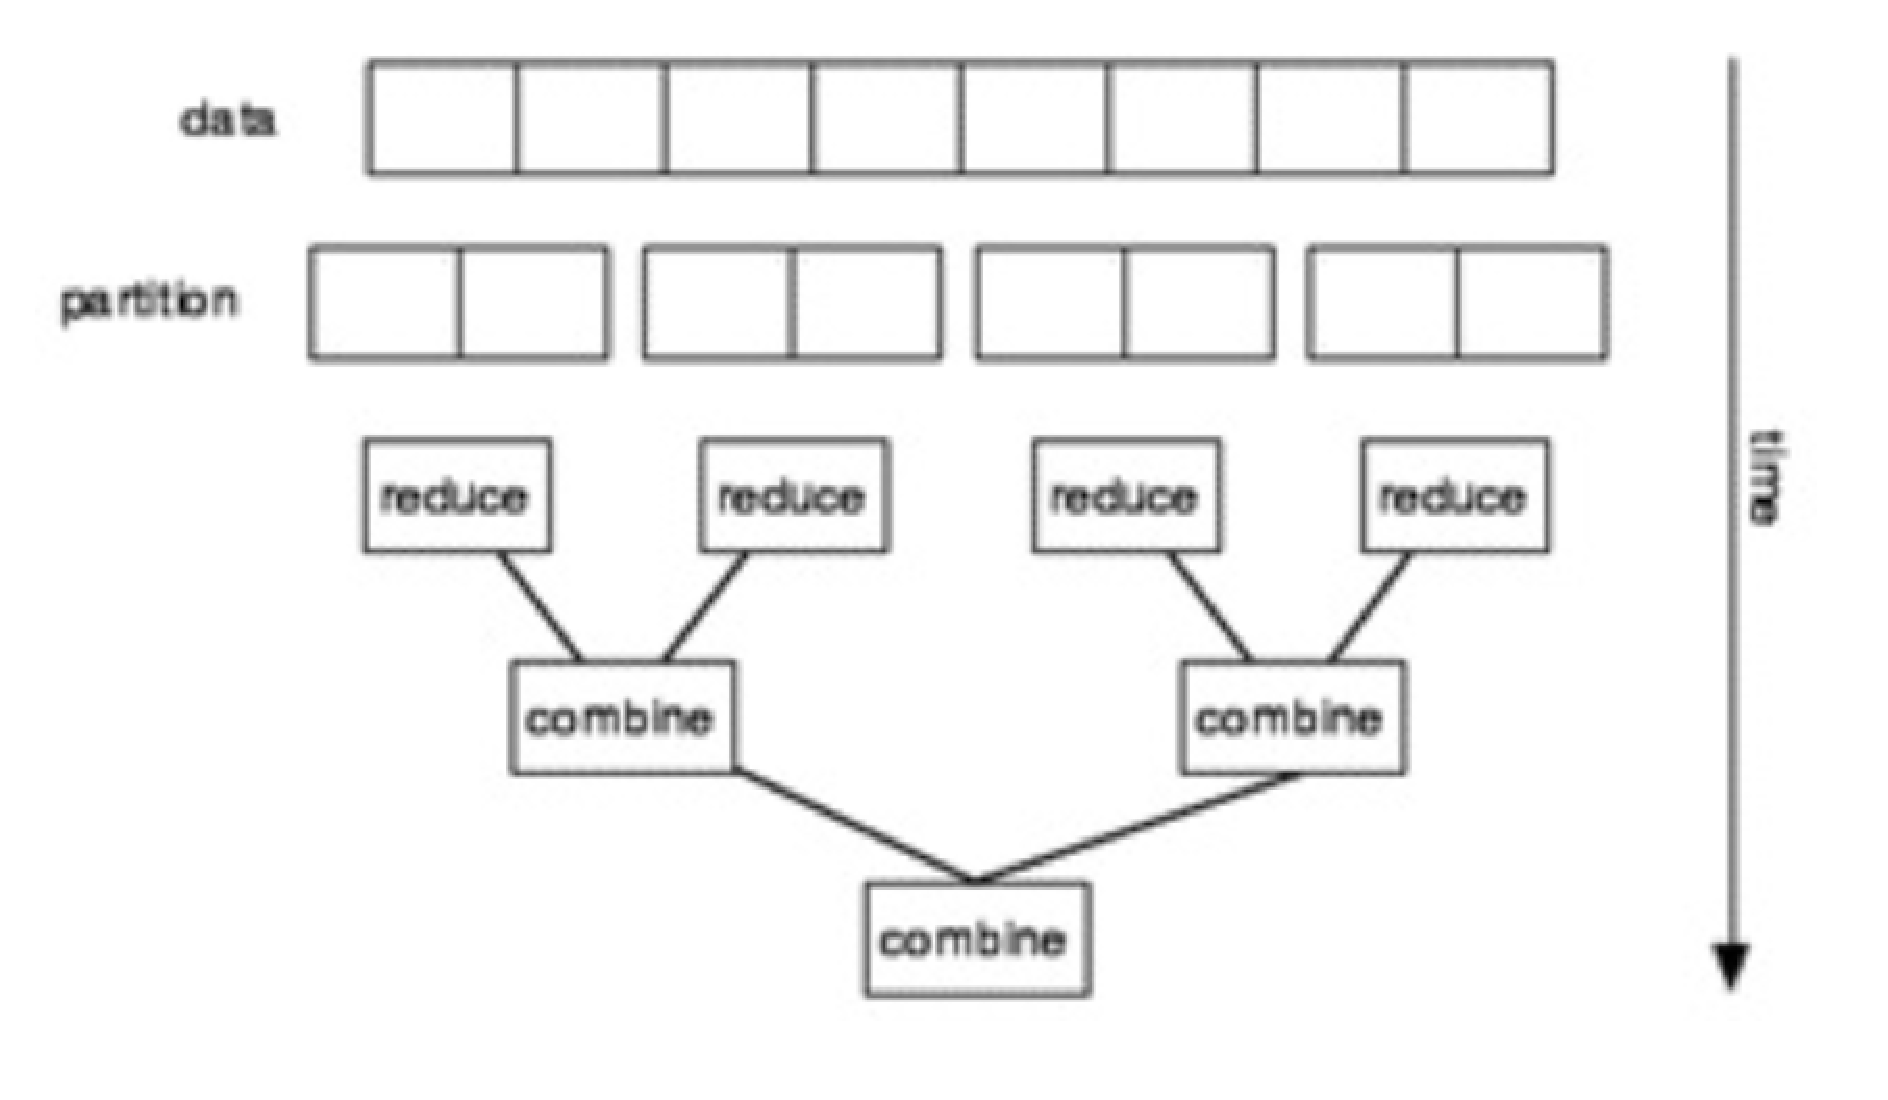
\includegraphics[width=12cm]{fig_05_005.eps}

先ほどの例に戻ると、\texttt{clojure.core.reducers}ライブラリを引き込み、reducerバージョンの関数を使って、ground-weightの計算を書き直すことができます。

\begin{lstlisting}[numbers=none]
(ns shipping.reducer
  (:require [shipping.domain :refer (ground?)]
            [clojure.core.reducers :as r]))

(defn ground-weight [products]
  (->> products
       (r/filter ground?)
       (r/map :weight)
       (r/fold +)))
\end{lstlisting}

この実装は、\texttt{clojure.core} 名前空間の代わりに \texttt{clojure.core.reducers} 名前空間の関数を使用する以外は、オリジナルバージョンと同様です。reducersの主な利点の1つは、他のアプローチと比較して、操作の構成可能な形状を維持することができることです。

フィルタとマップのリデューサーのバージョンは、元の積のベクトルに対して変換を実行しないことを思い出してください! 最終的に\texttt{fold}を呼び出すまで何も起こりません。この例では、reduceとcombineの両方のステージで同じ関数を使用する、最も単純なバージョンの\texttt{fold}を使用しています。

問題を再帰的に分割する並列計算では、以下のタイミングを決定する必要があります。分割と再合成は、単に作業を行うよりもコストがかかります。これは個々の計算の大きさに依存するため、最適な答えはない。\texttt{fold}関数では、分割サイズを指定することができ、デフォルトはグループあたり512要素(\texttt{+}などの単純な算術演算でうまくいくサイズ)です。より複雑な変換を行う場合は、より小さなパーティションサイズが有効でしょう。

今回はマルチコアマシンでのパフォーマンスを向上させるためにリデューサを使用するので、シーケンスとリデューサのパフォーマンスを比較してみましょう。

\subsection{Reducerの性能}

シーケンス版とリデューサ版を、どんどん大きな商品のベクターで走らせてみます。詳細を理解するために、2つのスケールでデータを見ることにします。次の図は、商品数(N)が32、128、512、2,048の場合の結果です。デフォルトのパーティションサイズは512なので、N <= 512の場合、実際には折りたたみは並列ではなく、1つのパーティションになります。これらのテストは、4つのハイパースレッドコア(8コアとして報告)を持つMacBook Proで実行されました。

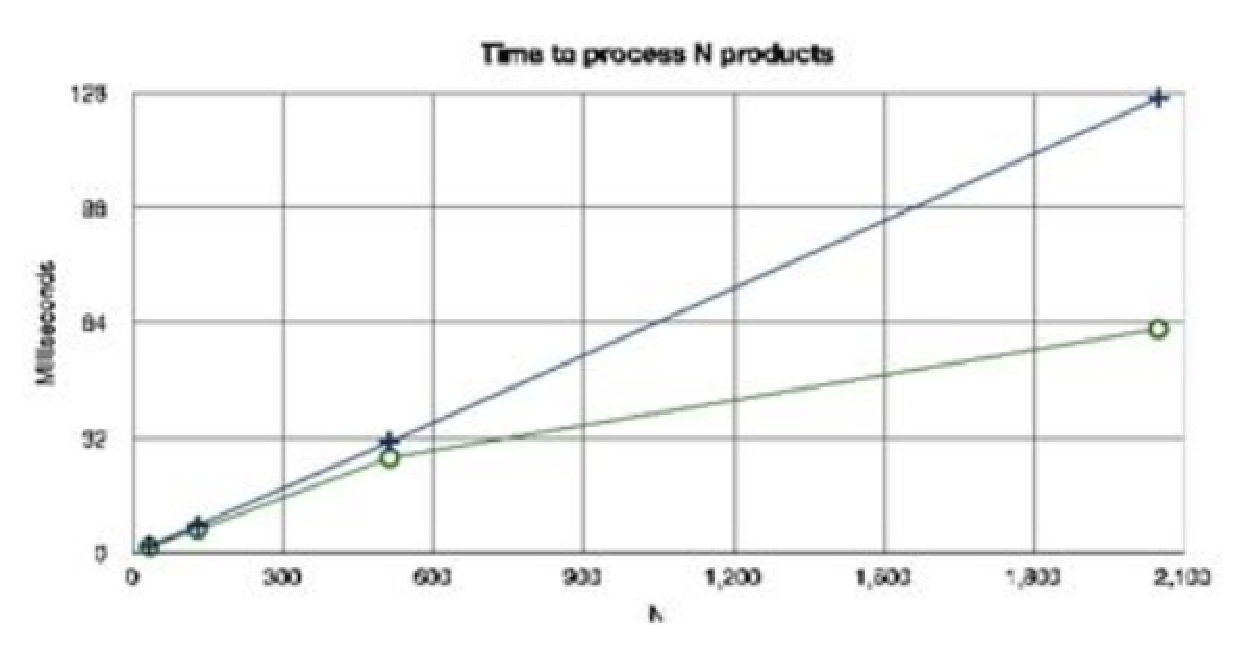
\includegraphics[width=10cm]{fig_05_006.eps}

予想通り、N=512まではシーケンス版とリデューサーの性能は同等である。しかし、パーティションサイズを超えると、シーケンス版はシングルスレッドですが、リデューサ版はデータをパーティションに分割し、異なるスレッドで並列実行されます。ここで一旦引いて、次の図にある3つのデータポイント(N=8,192, 32,768, 131,072)を追加して、Nの値が大きい場合の影響を見てみましょう。

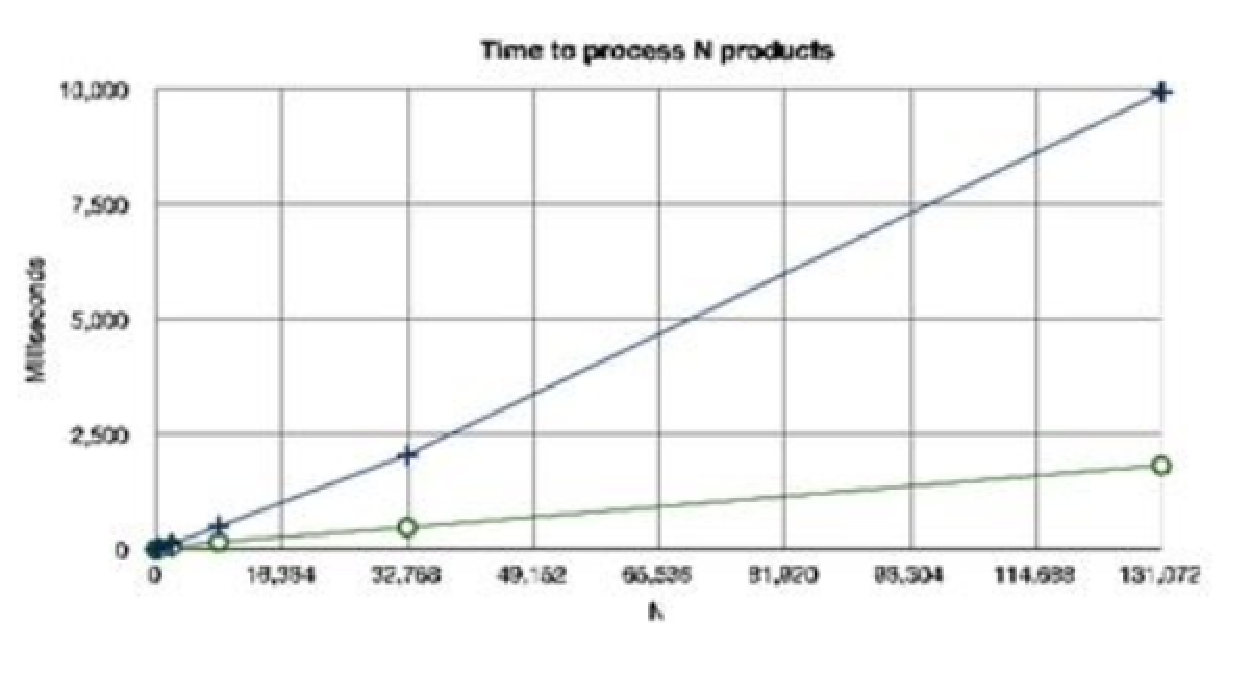
\includegraphics[width=10cm]{fig_05_007.eps}

Nが大きくなると、reducerの利点が明らかになる。reducerは4つの利用可能なコアに作業を分割するのに対し、シーケンスバージョンは1つのコアを使用するのである。さらに、reducer版ではゴミの発生が少ないので、ガベージコレクタの負荷が軽減されます。

reducerの主な利点の1つは、より多くのコアを持つマシンに移行したときに、同じコードがより速く実行されることです。マシンのコアの一部をオフにすることで、その違いをシミュレートすることができます。N=131,072 を固定し、コア数を変化させながら、シーケンスとreducerのテストを再実行してみましょう。このテストでは、ハイパースレッディングもオフにして、その影響を排除しています。

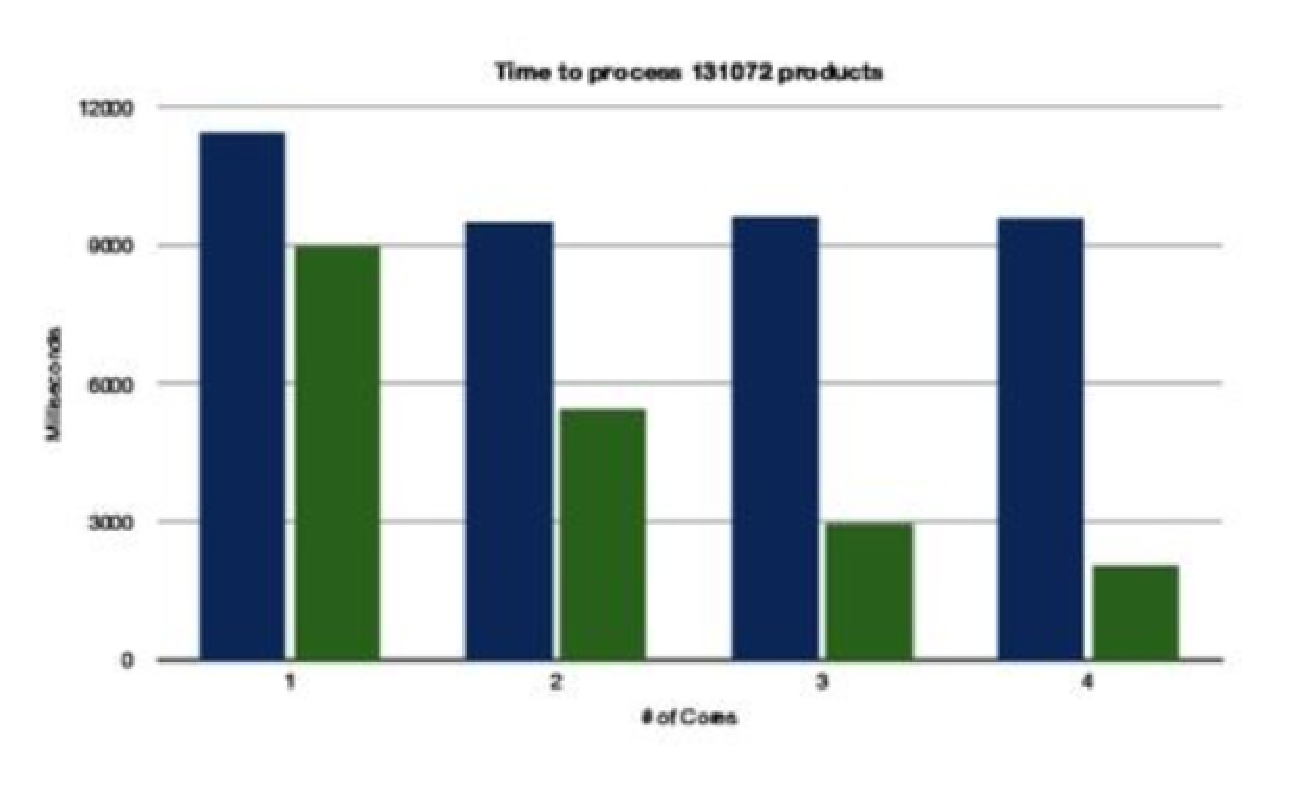
\includegraphics[width=10cm]{fig_05_008.eps}



前の図で、シーケンス版の性能はコア数に関係なく事実上同じであることがお分かりいただけると思います。シングルコアの場合は、ガベージコレクションやその他のマシン上の作業も唯一のコアを使用するため、特に悪化します。しかし、reducer版では、明らかに余分なコアの恩恵を受けており、同じコードが自動的に高速化されます。8コアや16コアのサーバーに移行すれば、このコードはさらに高速になると推測できます。

reducerを使うときは、データの大きさ、パーティションごとの作業の大きさ、想定するコア数を考えることが重要です。要素数がパーティションサイズより小さいときは、シングルスレッドになります(それでも穏やかな効果が見られるかもしれません)。パーティションサイズを超えると、reducerはマルチスレッドになりますが、オーバーヘッドが発生するため、コア数の倍数にはならない可能性があります。

もう1つのキーは、並列折りたたみ可能なコレクションは(現在ではもっと追加されるかもしれませんが)永続ベクトルと永続マップだけであることです。他のすべてのコレクション(およびシーケンス)は、1つのパーティション上のリダクションにフォールバックされます。このリダクションはより高速になる可能性がありますが、マルチスレッドにはなりません。

Reducerは、シーケンスライブラリの使いやすさと、fork/joinのマルチスレッド性能を併せ持つもので、両者の良いとこ取りのようなものです。reducers を最大限に活用するには、処理量が多く、データが折りたたみ可能なベクトルやマップとして存在する場合に限定して使用するようにしましょう。 % Parallelism with Reducers
\section{プロセスで考える}

これまで、一回限りの非同期(\texttt{future}や\texttt{promise})、粗粒度のタスク並列、細粒度のデータ並列のためのコアの使い方をみてきました。しかし、時には並列性よりも並行性に興味を持つことがあります。つまり、プログラムを一連の同時実行スレッドとして設計する能力です。また、これらのスレッド間で、一度だけでなく、時間の経過に伴う一連の値として、値を伝達したいと思うこともあるはずだ。

\texttt{core.async}ライブラリは、このようなニーズに対する回答として作成された。当初はClojure自体の一部として構想されましたが、最終的にはコア言語よりも迅速な進化を可能にするために、独立したライブラリとしてリリースされました。\texttt{core.async}ライブラリは、goブロック(独立した実行スレッド)とチャネル(ある場所から別の場所に値を渡す手段)という2つの中心的な概念を提供します。次に、これらの使い方を探ります。


\subsection{チャネル}

チャネルは、プログラムの2つ以上の部分の間で一連の値を時間的に伝達するための待ち行列のような手段です。チャネルは、スレッド間で作成したり受け渡ししたりすることができます - ステートフルです。

チャネルは、チャネル内の値を保持するためにバッファを使用します。デフォルトでは、チャネルはバッファなし(長さゼロ)で、Javaの\texttt{SynchronousQueue}に似ています。バッファされていないチャネルは、producer と consumer の両方がチャネルに値を渡すことができるようになるまでブロックされます。\texttt{core.async} ライブラリは,固定長のバッファ,ドロップバッファ(新しいデータが一杯になったらドロップする),スライディングバッファ(古いデータが一杯になったらドロップする)も提供します.

\texttt{core.async} でチャネルを作成するには、\texttt{chan} 関数を使用します。以下は、異なるバッファタイプとサイズのチャネルを作成する例です。

\begin{lstlisting}[numbers=none]
(require '[clojure.core.async :refer
 (chan dropping-buffer sliding- buffer)])

(chan) ;; unbuffered (length=0)
(chan 10) ;; buffered (length=10)
(chan (dropping-buffer 10)) ;; drop new values when full
(chan (sliding-buffer 10)) ;; drop old values when full
\end{lstlisting}

どんな典型的なClojure値でもチャネルに入れることができ、相手側に伝達されます。1つの例外は \texttt{nil} で、これはチャネルが閉じられ、それ以上データが残っていないことを示すために使用される特別な値です。チャネルは,\texttt{close!}関数で閉じられます.

チャネルに対する最も重要な操作は \texttt{put} と \texttt{take} の 2 つであり、それぞれコンテキストや用途に応じていくつかの形式があります。通常のスレッドからチャネルを使用する場合、\texttt{put} 演算子は \texttt{>!!}、\texttt{take} 演算子は \texttt{<!!} となります。以下は,チャネルを作成し,そこに値を入れ,取り出す例です.

\begin{lstlisting}[numbers=none]
(require '[clojure.core.async :refer (chan <!! >!!)])

(def c (chan 1))
(>!! c "hello")
(println (<!! c))
\end{lstlisting}

前述のコード例では、\texttt{put}と\texttt{take}の両方の操作を現在のスレッドから行っていますが、実際のプログラムでは、チャネルの両端は通常、異なるスレッドまたはコンポーネントから使用され、それらの間で値が送信されるようになっています。また、サイズ 1 のバッファを持つチャネルを作成したことにお気づきでしょうか。もしバッファのないチャンネルを使っていたら、この例では put の待ち時間がブロックされ、この例が完了するのを妨げていたでしょう。

\texttt{core.async} のチャネルは決して unbounded ではありません。これは、後で問題になるようなアーキテクチャ上の問題を避けるための、意図的な設計上の制約です。システム内の未束縛のキューは、予期せぬ負荷が積み重なり、最終的にはリソースを使い果たし、システムをクラッシュさせる場所となります。

その代わりに、\texttt{core.async}では、固定サイズを選択するか、バッファがいっぱいになったときに何をドロップするかのポリシーをインスタンス化することで、バッファの長さを制限することを要求します。固定サイズのバッファは、満杯のキューに追加しようとするとプロデューサーをブロックさせるので、バックプレッシャーを発生させます。これは、実稼働時ではなく、前もっての設計思考を促すものです。システムは、負荷がなくなるのを待つか、仕事を減らすことを受け入れるか、どの仕事をしないかを選択することによって、明示的にブロックに対処するように設計されていなければなりません。

チャネルを別のサブシステムの専用スレッドから完全に使用することも可能ですが、Goブロックから使用するのが一般的です。Goブロックを使うと、スレッドのプールで対応できる軽量な処理ループを作ることができます。

\subsection{Goブロック}

伝統的に、Java(またはClojure)プログラムは、プログラムの各部分の実際の処理を含むスレッド(実際のオペレーティング・システムのスレッドに対応する)を作成します。\texttt{core.async}ライブラリは、C. A. R. HoareのCommunicating Sequential Processes (CSP) [Hoa78]の遺産に基づく、異なる伝統に従います。

この研究の詳細については、ここでは触れません。重要なことは、プログラムをどのように構成するかについて、異なる方法で考えることを学ぶことです。スレッドは希少で高価な資源です。スタックスペースやその他の資源を消費し、起動も比較的遅いです。スレッドがI/Oのためにブロックされると、これらのシステムリソースを浪費することになります。

その代わりに、\texttt{core.async}は、スレッドプールにマッピングされ、作業の準備ができたときにだけ実行される軽量なプロセスという観点から考えることを推奨しています。チャネルへのメッセージの出入りを待つ間にブロックする代わりに、プロセスが再び実行できるようになるまで、これらのプロセスを停止させることができます。これによって、やるべきことがあるときだけプロセスを実行することができる。また、複数の I/O 操作にまたがって選択し、最初の操作が完了したときに処理を進めるという、興味深い新しい動作を実装することも可能です。

\texttt{core.async}では、これらのプロセスをGoブロックと呼んでいます(Go言語の同様の概念にちなんでいます)。goブロックの中ではチャネルを使いますが、\texttt{put}と\texttt{take}の操作は \texttt{<!} と \texttt{>!} です。

以下は、メッセージを受信し、それを表示する処理を行うgoブロックを作成する関数の例です。

\begin{lstlisting}[numbers=none]
(require '[clojure.core.async :refer (go <!)])

(defn go-print
  "チャネル c からメッセージを取り出し、表示する。"
  [c]
  (go
    (loop []
      (when-some [val (<! c)]
        (println "Received a message:" val)
        (recur)))))
\end{lstlisting}

この例では、goブロックは軽量なプロセスとして実行されます。チャンネル操作(\texttt{<!} や \texttt{>!} など)に到達したとき、そのチャンネル操作が可能であれば実行を継続する。チャンネル操作が継続できない場合、go ブロックはパークされます。パークされたgoブロックはスレッドを消費せず、事実上、データを待つために中断された計算となります。チャネル操作が続行できるようになると、goブロックは実行を継続するために起動します。

Goブロックは、プログラムを潜在的な同時処理に分割するための素晴らしいツールです。\texttt{core.async}がgoブロックとチャネルで特によくサポートする使用例は、データ変換ステージのパイプラインを構築することです。

\subsection{パイプライン}

\texttt{core.async}ライブラリは,2つのチャンネルを並列変換ステージで接続するための関数群,すなわち\texttt{pipeline},\texttt{pipeline-blocking},\texttt{pipeline-async}を提供します.このパイプライン関数は、入力チャネルから出力チャネルに値を移動しますが(より単純な\texttt{pipe}と同様)、重要な追加機能を提供します:トランスデューサの並列実行です。

この機能により、パイプラインはチャネルで区切られたデータ変換ステージを作成するのに適しています。並列実行により、データパイプラインを線形に記述しながら、コアをフル活用することができます。各トランスデューサステージは多くの変換を組み合わせることができるため、どのように並列化するか、どこでチャネルを分離するのが有効か、多くの選択肢があります。

例えば、ソーシャルメディアのメッセージのストリームを処理するシステムを考えてみましょう。トランスデューサーとして定義された一連の変換を提供することができます。

\begin{lstlisting}[numbers=none]
;; メッセージを単語の集合に解析する
(def parse-words
  (map #(set (clojure.string/split % #"\s"))))
;; 単語を含むメッセージをフィルタリングする
(def interesting (filter #(contains? % "Clojure")))
;; 異なる単語リストに基づいて感情を検出
(defn match [search-words message-words]
  (count (clojure.set/intersection search-words
                                   message-words)))
(def happy
  (partial match
           #{"happy" "awesome" "rocks" "amazing"}))
(def sad (partial match #{"sad" "bug" "crash"}))
(def score (map #(hash-map :words %1
                           :happy (happy %1)
                           :sad (sad %1))))
\end{lstlisting}

これらのトランスデューサは、入力ストリームから出力ストリームまで1段のパイプラインで一緒に構成することができます。


\begin{lstlisting}[numbers=none]
(defn sentiment-stage
  [in out]
  (let [xf (comp parse-words interesting score)]
    (async/pipeline 4 out xf in)))
\end{lstlisting}

これは、最大4つの並列スレッドで \texttt{in} と \texttt{out} を接続し、それぞれが結合されたトランスデューサの変換を処理します。しかし、センチメント分析が行われている間に、アーカイブへのロギングなど、別のパイプラインステージで発生する可能性のある他の分析があるかもしれません。その場合、このステージを2つに分割し、センチメント解析の前に新しい中間チャネルを作成することができます。

\begin{lstlisting}[numbers=none]
(defn interesting-stage
  [in intermediate]
  (let [xf (comp parse-words interesting)]
    (async/pipeline 4 intermediate xf in)))

(defn score-stage
  [intermediate out]
  (async/pipeline 1 out score intermediate))

(defn assemble-stages
  [in out]
  (let [intermediate (async/chan 100)]
    (interesting-stage in intermediate)
    (score-stage intermediate out)))
\end{lstlisting}

現在では、受信したメッセージをすべて受け取り、興味深いものだけを出力する第一ステージ(最大4スレッドを使用)と、興味深いメッセージを受け取り、スコアをつける第二ステージがあります。量が少ないので、第2ステージの並列度を1スレッドに減らすことができます。これらのステージを組み立てると、中間メッセージチャネルを他の目的に使用する機会も得られます。

トランスデューサーはコンポーザブルなので、1つのステージに積み重ねることもできますし、ステージをまたいで分割することも可能です。各ステージの並列度は独立して変化させることができる。これは、効率的なデータ処理パイプラインを構築するための強力な技術です。パイプラインは、きめ細かなデータ並列処理の性能を犠牲にすることになりますが、より柔軟なアーキテクチャを実現することができます。


 % Thinking in Processes
\section{まとめ}

ムーアの法則に従ってトランジスタ数が増え続けるのは確かだが、それに伴うクロック速度の向上はもはや期待できない。その代わり、チップあたりのコア数は増え続けている。これからは、より多くのコアが利用可能になったときに、それを自動的に活用できる言語が求められているのです。

これまで、より多くのコアを利用して、より多くの作業を行うことができる分野をいくつか取り上げてきました。まず、futureを使ってバックグラウンドスレッドで非同期処理を行うことを考えてみました。Futuresは、非同期タスクを実行し、場合によってはその結果を通信で返す必要がある場合に、最初に選択すべきものです。もし、複数の値や非同期タスクの任意の場所からの配信が必要な場合は、promiseを使用してください。非同期タスクが状態を保持する必要がある場合(シミュレーションなど)、agentが最適です。

もし、あなたのシステムが仕事やリクエストの受信キューとして構成されているなら、その仕事をキューで受け入れ、ワーカスレッドのプールに送って処理する必要があります。そのためには、標準的なJavaライブラリのツールを使って、キュー、スレッド、エグゼキュータを使ってシステムを構成してください。

データが大きなベクトルやマップになっている場合は、reducerを使ってデータセット全体に対して並列に動作するように計算を構成する必要があります。reducerはシーケンス関数に期待されるような複合化能力を持ちながら、マシンの全コアをフルに活用することができ、中間オブジェクトを避けることでガベージコレクションを最小限に抑えることができます。

並行処理についてまだ調べていないことのひとつに、成長するシステムをいかにして断片化するかがあります。コンポーネント間の長寿命な接続を作成するために、再び core.async を活用することができます。次に、完全なアプリケーションを構築するために、これらのコンポーネントをどのように構築するかに焦点を当てます。


Footnotes
[19]
http://dl.acm.org/citation.cfm?doid=828.833 % Wrapping Up % Use Your Cores
\chapter{コンポーネントの作成}

ドメインの表現、集計データの作成、関数によるデータ変換、状態の作成、並行処理の使用など、基礎は固まりました。次は、より大きな単位で、問題に対応するコードの構築を始める番です。この大きな単位をコンポーネントと呼ぶことにします。コードをコンポーネントに分割することで、問題に対応する部分をより高いレベルで考えることができるようになります。また、コンポーネントの境界は、複数の開発者やチームにコードベースを分割するのに適した方法です。また、再利用の機会にもなり得ます。

コンポーネントは、より細かい要素(関数、レコード、プロトコル)の集合体であり、全体として大きな目的を持っている。呼び出し元が使用する外部APIを備えている。また、コンポーネントの状態を含む内部実装を持ち、内部で並行処理を行い、データを並列処理したり、イベントに対応するための別スレッドを作成したりすることもできます。

アプリケーションの機能をClojure名前空間に整理する方法を見て、コンポーネントの考察を開始します。これは、コンポーネントの内部と外部の両方を含むすべてのコードに適用されます。次に、呼び出し元が使用する外部APIについて見ていきます。これは、関数呼び出しインターフェースと、より長寿命の \texttt{core.async} チャンネルの使用の両方を考慮する必要があります。最後に、コンポーネントの内部をどのように実装するか、状態や並行性のために既に見たツールを使ってコンポーネントの状態やそのライフサイクルを管理するかについて見ていきます。

第7章「アプリケーションを構成する」では、これらのコンポーネントを次のステップとして、アプリケーションを完全に組み立てていきます。


\section{名前空間による整理}

Clojureコードは、一連の個々のトップレベル・フォーム(関数、レコード、プロトコルなど)としてコンパイルされ評価されますが、Clojureはそれらの個々のフォームをグループ化するための名前空間を提供します。名前空間は、フォームのグループを収集し、整理し、名前を付けるために使用できる、名前付きの階層的なコンテナです。名前空間の実用的な使い方の1つは、どこかで同じ名前と衝突することを心配することなく、コードで単純な名前を使えるようにすることです。名前空間は、どれを意味しているのかを指定する手段を提供します。

Clojureのコードはより細かい要素で構成されていますが、依存関係は関数レベルではなく、名前空間レベルで宣言され、読み込まれます。各名前空間の \texttt{ns} マクロは、その依存関係を定義し、まとめて依存関係グラフを作成する。この依存関係グラフは、名前空間がロードされる順序に影響を与える。名前空間がマルチメソッドやプロトコル(いずれも型固有の動作のためのオープンシステム)の実装を提供する場合、実装を使用する前にロードする必要があるため、このロード順序が重要になることがあります。

名前空間とコンポーネントは、どちらも組織化のためのツールである。名前空間は機能を整理するための言語機能であり、コンポーネントは問題レベルで整理するための手段である。この2つのアプローチは、どちらも有用であり、連動してコードを構造化し、最終的に他の開発者が理解しやすく、使いやすくするものです。

\subsection{名前空間のカテゴリ}

Clojureで関数のセットを名前空間にグループ化するのは、多くの理由があります。以下のカテゴリは、アプリケーションを反映した論理的な名前空間アーキテクチャを作成するために使用することができます。

\begin{description}
\item [Utility] utility名前空間は、ドメインや目的別に整理された汎用的な関数を提供します。例えば、文字列操作や特定のファイル形式の解析のための名前空間を作成することができます。一般に、utility名前空間は依存関係がほとんどありません。
\item [Data definition] カスタムコレクションやドメインエンティティのセットを、コレクションやエンティティを使用するためのヘルパー関数と一緒にネームスペースで定義するのが一般的である。
\item [Abstraction] プロトコルのような抽象的なものは、最小限の依存関係でネームスペースに分離することができます。
\item [Implementation] 一方、プロトコルやインタフェースで定義された抽象化機能を名前空間で実装すると便利なことが多い。この実装は、アプリケーションに組み入れることができる。
\item [Assembly] 実装のセットと、実装をどのように構築し接続するかを指定する構成がある場合、assembly名前空間がすべてを結びつけます。実装の内部では、一般に抽象化(プロトコル)またはデータ構造のみが直接使用される。
\item [Entry point] ほとんどのアプリケーションには、アプリケーションの開始(設定の収集を含む)とアセンブリや他のライフサイクル操作の開始をつなぐ1つ以上のエントリーポイントがあります。
\end{description}

次の図は、ライブラリやアプリケーションの中で、これらの種類の名前空間がどのように一般的に重なり合っているかを示しています。

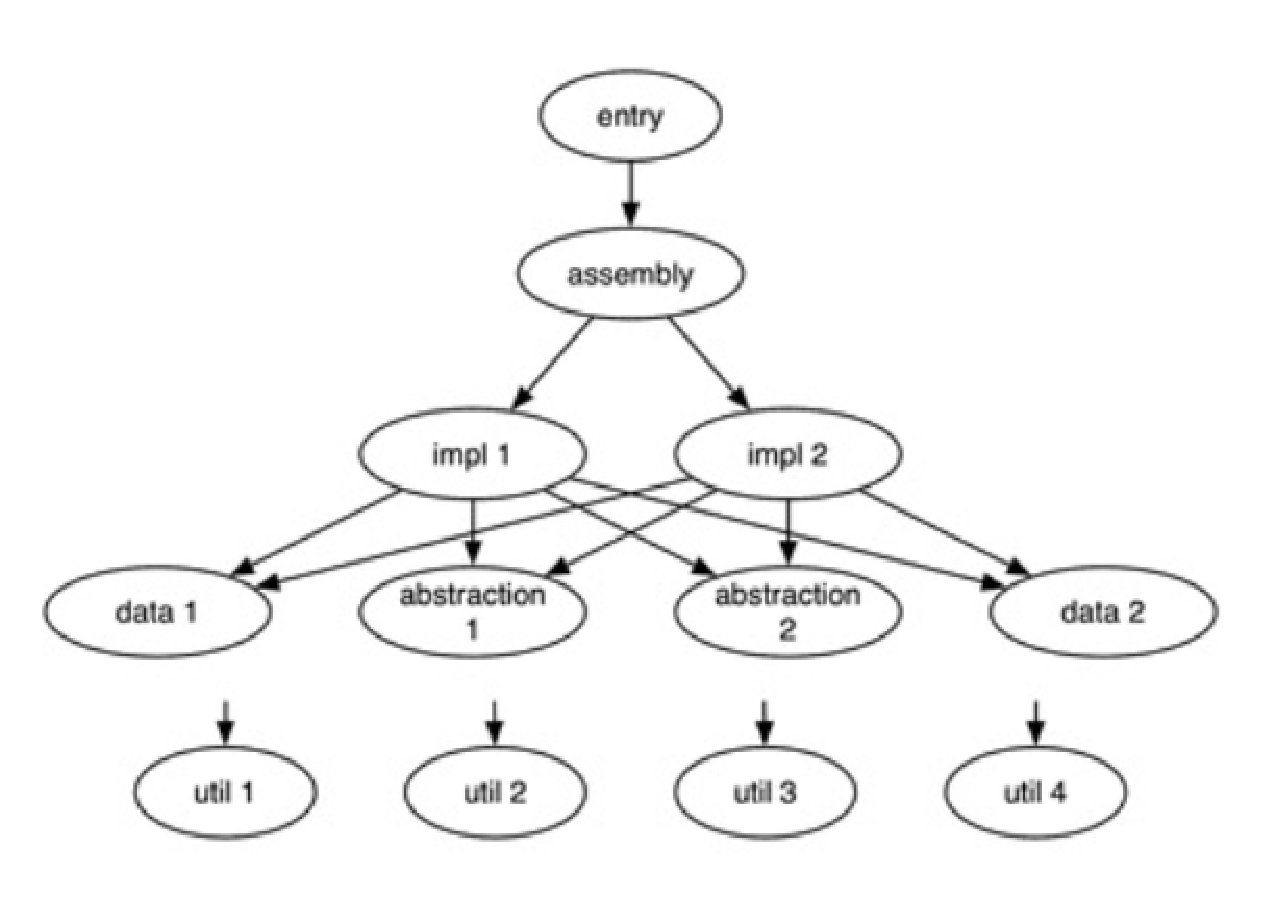
\includegraphics[width=10cm]{fig_06_001.eps}

この構造は、独自の名前空間構造を設計する際のガイドラインとして有効である。ユーティリティ名前空間は依存関係グラフの一番下にあり、それ自身の依存関係はほとんどなく、上の複数の名前空間によって使用されています。次の層は、データまたは抽象化名前空間のいずれかからなり、アプリケーション自体のビルディングブロックを作成します。抽象化の上には、その抽象化のための実装があります。その上には、設定が処理され、実装が組み立てられて接続され、 アプリケーションの状態が作成されるアセンブリ層があります。一番上には、ウェブアプリケーション、コマンドラインインターフェース、サービスなど、一つまたは複数のエントリーポイントがあります。

プロジェクト内の名前空間を名前空間ツリーとして整理するには、さまざまなアプローチがありますが、唯一の正解はありません。小規模なプロジェクトでは、ネームスペースの大部分をプロジェクトにちなんだ単一のルート内に配置し、ネストを最小限にすることがよくあります。

\begin{lstlisting}[numbers=none]
myproject.util.string ;; utility
myproject.util.json ;; utility
myproject.domain    ;; data - domain entities
myproject.config    ;; data - config data
myproject.services  ;; abstraction - service definitions
myproject.impl.xyz  ;; implementation of service abstraction
myproject.assembly  ;; assembly
myproject.main      ;; main entry point - command-line
\end{lstlisting}

小規模なシステムでは、多くの抽象化機能、実装、ユーティリティをグループ化して、サービスを水平方向に切り分けるのが最も簡単な場合があります。システムが大きくなるにつれて、システムを縦割りにして、それぞれのコンポーネントをAPI、実装、データ定義のセット、ユーティリティで構成することがますます有用になってきます。

\subsection{パブリックとプライベートの関数}

Clojureは、データや関数をデフォルトで利用できるようにすることに偏っています。しかし、ほとんどの名前空間には、ヘルパーとして使用される関数や、決して一般的な使用方法の一部となることを意図していない関数があります。名前空間内の関数を定義するときは、消費者がそれらの関数をどのように認識し、どのように使用することが期待されるかを考えてください。いくつかのツールや規約は、プライベートvar、ドキュメント文字列、そして名前空間の構造そのものです。

Clojureに組み込まれた主要なツールは、 \texttt{defn-} または \texttt{\^:private} メタタグを使用して関数をプライベートとしてマークする機能です。


\begin{lstlisting}[numbers=none]
(defn- internal-function [] ...)
(def ^:private internal-constant 42)
\end{lstlisting}


これらのvarはいくつかの名前空間関数の結果から省略されますが、それでもreader var構文で直接アクセスしたり、名前空間オブジェクトを直接呼び出したりすることは可能です。

autodocのようなドキュメント生成ツールは、docstringを持たない関数を省略することがあります。Clojureコア自身は、高度なClojure開発には有用ですが、一般的な使用には適さない内部関数を強調しないためにこの機能を使用します。

最後に、 \texttt{myproject.internal.db} のような名前空間を使用して、内部であることを明示的にマークするのはよくあることで、 \texttt{internal} 以下のすべての名前空間は非パブリックとみなされます。

これらのテクニックは、自分のコードの利用者にどこから手をつければよいかを示すのに役立つと思われます。

さて、名前空間をどのように整理すればいいのかがわかったところで、 それらの名前空間を使っていくつかのコンポーネントを作成してみましょう。まずはコンポーネントのAPIをどのように設計するかを考えてから、コンポーネントをどのように実装するかを考えていきます。






 % Organizing with Namespaces
\section{コンポーネントAPIの設計}

アプリケーション内でコンポーネントを特定する場合、そのコンポーネントがどのような目的を持ち、他のコンポーネントからどのように使用されるかを考えることから始める必要があります。代表的なコンポーネントには、情報管理、プロセッサ、ファサードなどがあります。情報マネージャーは、メモリ内または外部のデータストアにある状態を追跡し、データの作成、変更、問い合わせの操作を提供します。プロセッサーは、データの変換や計算を行うコンポーネントである。ファサードコンポーネントは、主に別の外部システムにアクセスできるようにする(プラグイン可能な)ために存在します。

実際には、ほとんどのコンポーネントはこれらの箱にきれいに収まるわけではなく、1つまたは複数の側面を組み合わせて、独自のアプリケーションのユニークなニーズを満たすコンポーネントにします。

コンポーネントを設計する際に最初に考慮すべきことは、外部の消費者が使用するAPIです。コンポーネントとの対話には、主に2つの方法があります。関数を呼び出す方法と、キューやチャネルでメッセージを渡す方法です。まず、関数について見てみましょう。

\subsection{関数によるコンポーネントデータの操作}

API関数は、外部の消費者がコンポーネントと対話できるようにするための、ノブ、ボタン、またはゲージのようなものです。Clojureでは、多くのものがユーザーによって関数として呼び出されますが、関数、マクロ、プロトコル、マルチメソッドなど、異なる実装があります。(他のもの-マップ、セット、キーワード、シンボルなど-はAPIの一部としてあまり有用ではありません)。

コンポーネントレベルに焦点を合わせましたが、これまで学習したことをすべて覚えておく必要があります。可能な限り、コンポーネントはイミュータブルなデータを直接公開すべきです。イミュータブルであるため、コンポーネントのデータの一部をコンシューマーに渡しても害はありません:コピーは必要ありませんし、コンポーネント自身のデータが影響を受けることもありません。呼び出し元がデータを手に入れたら、自由にClojureツールを使ってクエリや変換を行うことができます。

リクエストを受け取り、自動応答を形成するために使用されるルールのセットを管理する知識エンジンのコンポーネントを考えてみましょう。ルールの具体的なフォーマットはひとまず置いておいて、各ルールがデータとして定義されていると仮定します。ルールを追加、置換、削除するためのAPI関数と、何らかの基準に基づいてルールを検索するための関数が必要です。また、ルールを起動し、手元の作業を行うための関数も必要である。

\begin{lstlisting}[numbers=none]
;; 注:keはステートフル知識エンジン・コンポーネントを指す
;; Read interface
(defn get-rules [ke])
(defn find-rules [ke criteria])
;; Update interface
(defn add-rule [ke rule])
(defn replace-rule [ke old-rule new-rule])
(defn delete-rule [ke rule])
;; Processing interface
(defn fire-rules [ke request])
\end{lstlisting}

そして、これらの関数を次のように使うことができる。

\begin{lstlisting}[numbers=none]
(defn example [] (let [ke (new-ke)]
    (add-rule ke :r1)
    (add-rule ke :r2)
    (add-rule ke :r3)
    (replace-rule ke :r1 :r1b)
    (delete-rule ke :r3)
    (get-rules ke)))
\end{lstlisting}

しかし、もう少し深く見てみると、より小さな関数の集合でAPI全体をサポートできることがわかります。

\begin{lstlisting}[numbers=none]
;; Get the rule-set
(defn get-rules [ke])
;; Transform from one rule-set to another
(defn transform-rules [ke update-fn])
;; Produce a response from a request
(defn fire-rules [ke request])
\end{lstlisting}

\texttt{find-rules}関数は\texttt{get-rules}に対するフィルタリングとして実装することができる.\texttt{add-rule}、\texttt{replace-rule}、\texttt{delete-rule}関数はすべて、ルールセット全体に対する\texttt{transform-rules}の適用と見なすことができる。

ほとんどのAPIはこのパターンを持っている。つまり、少数の重要な基本関数と、使いやすさのために提供されるより大きな関数群である。プロトコルは、複数の実装がそのプロトコルを拡張できるように、機能の中核となるセットを捕捉する良い方法である。派生機能はAPIネームスペースで提供され、プロトコルの上にレイヤー化されるべきである。API関数は、プロトコルを拡張するあらゆるエンティティで動作する。

これを完全な名前空間にまとめると、次のようになる。

\begin{lstlisting}[numbers=none]
(ns components.ke)

;; SPI protocol
(defprotocol KE
  (get-rules [ke] "Get full rule set")
  (transform-rules [ke update-fn]
    "Apply transformation function to rule set. Return new KE.")
  (fire-rules [ke request]
    "Fire the rules against the request and return a response"))

;; private helper functions
(defn- transform-criteria [criteria]
  ;; ...
  )

;; api fns built over the protocol
(defn find-rules
  [ke criteria]
  (filter (transform-criteria criteria) (get-rules ke)))

(defn add-rule
  [ke rule]
  (transform-rules ke #(conj % rule)))

(defn replace-rule
  [ke old-rule new-rule]
  (transform-rules ke #(-> % (disj old-rule) (conj new-rule))))

(defn delete-rule
  [ke rule]
  (transform-rules ke #(-> % (disj rule))))
\end{lstlisting}

この実装では、図にあるように、小さな拡張可能な抽象化(サービスプロバイダインタフェース)の上にコンポーネントAPIを重ねる形で定義しています。

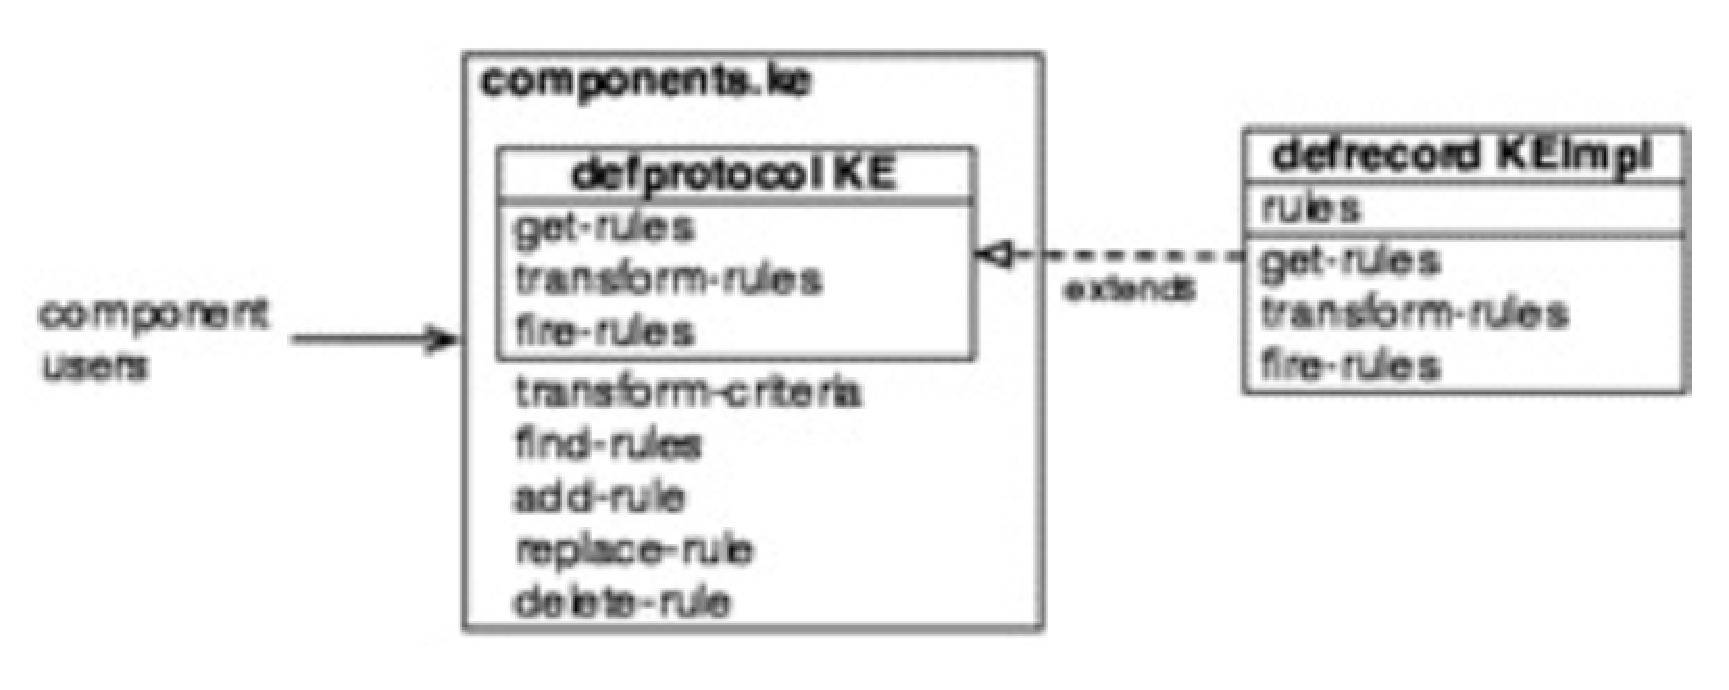
\includegraphics[width=10cm]{fig_06_002.eps}

API全体のプロトコルを作成すると、どのような実装でもすべての関数を再実装する必要があります。その代わり、Clojureで関連する関数のセットを収集するための最適なツールは、プロトコルではなく名前空間です。プロトコルは、今回のように拡張のための最小限の抽象化を定義しているときに最適です。

このコンポーネントの状態実装部分については後で説明し、今は非同期呼び出しなど、他のAPIに関する考察に焦点を合わせます。


\subsection{非同期API}

第5章「コアを使う」では、非同期API関数に対して1回限りの非同期応答を提供するためのfuturesやpromiseといったツールについて既に説明しました。前のセクションで出てきた \texttt{fire-rules} 関数を考えてみましょう。レスポンスを生成するのに時間がかかるかもしれないので、呼び出し元をブロックするのではなく、futureを返すこともできます。

\begin{lstlisting}[numbers=none]
  (let [response-future (fire-rules ke request)]
    ;; ... other work...
    @response-future) ;; レスポンスを取得するために参照する
\end{lstlisting}

応答のためにブロックするのではなく、futureを返すことで、呼び出し側がブロックするタイミングを選択できる(futureをdereferencingすることで)。もう一つの選択肢は、ここに示すように、コールバックを受け取るか(関数を呼び出す)、プロミスを返すか(結果を提供する)である。


\begin{lstlisting}[numbers=none]
;; 知識エンジンが起動するfire-rulesにコールバックを送る。
(let [callback (fn [response] ...)]
  (fire-rules ke request callback))

  ;; 知識エンジンが応答を返すために使うpromiseを送る
(let [result-promise (fire-rules ke request)]
  ;; 必要なときにresult-promiseを参照する。
  @result-promise)
\end{lstlisting}

非同期API呼び出しにどちらが適しているかは、APIそのものよりも呼び出し側のコードに依存します。

さて、直接または非同期の関数呼び出しでAPIを作成する方法を見てきましたが、アプリケーションの寿命を通じてより永続的な関係でコンポーネントを接続する方法についても検討する必要があります。






 % Designing Component APIs
\section{チャネルを使ったコンポーネントの接続}

コンポーネントは、プロデューサコンポーネントからコンシューマコンポーネントに値を供給するために、継続的な一連の値を渡すために接続する必要があるかもしれません。 \texttt{core.async} チャネルは、このような目的に最適です。コンポーネントが値の入出力にチャネルを必要とする場合、そのコンポーネントは外部のチャネルを受け入れるか、内部でチャネルを作成して利用できるようにします。

例えば、ソーシャルメディアからのメッセージを受信するコンポーネントがあるとします。一つの選択肢は、コンポーネントがその構成の一部として着信チャネルを受け入れることでしょう。

\begin{lstlisting}[numbers=none]
(defn make-feed-processor
  "指定された入力チャネルに新しいフィードプロセッサを作成します。"
  [input-channel] ,,,)  
\end{lstlisting}

あるいは、feed-processorが自らチャネルを構築し、ユーザーがそれを要求できるようにすることもできます。

\begin{lstlisting}[numbers=none]
(defn make-feed-processor
  "新しいFeed Processorを作成する"
  []
  (let [ch (async/chan 100)] ,,,))

(defn input-chan
  "feed processorの入力チャネルを返します。"
  [feed-processor] ,,,)
\end{lstlisting}


ほとんどの場合、外部チャネルを受け入れることで、第7章「アプリケーションの構成」で説明するように、後でシステムを組み立てるための最も多くのオプションが生まれます。ここで決定すべき重要なことのひとつに、入力チャネルのバッファリングポリシーがあります。もしコンポーネントが内部で入力チャネルを作成するのであれば、この決定を行わなければなりません。もし設定可能である必要があるのなら、コンポーネントはバッファ設定オプションを公開する必要があります。チャネルを外部で作成する場合は、システムのアセンブリコードがシステムの残りの部分と一緒に自由に設定することができます。

どちらの場合でも、チャネルを持つコンポーネントができたら、それらをさまざまな方法で接続する必要があります。\texttt{core.async}は多くの種類のチャネルコネクタを提供します。ここでは、それらを直接接続、ファンイン、ファンアウトの観点から分類してみます。

\subsection{ダイレクトコネクション(1対1)}

内部で構築されたチャネルを提供する2つのコンポーネントを組み合わせる場合、直接接続が必要になることがあります。2つのコンポーネントを一緒に使うには、この例のようにチャンネルをパイプで接続します。


\begin{lstlisting}[numbers=none]
(let [component1 (make-comp-1)
      output-chan (get-output component1)
      component2 (make-comp-2)
      input-chan (get-input component2)]
  (pipe output-chan input-chan))
\end{lstlisting}

ここでは、 \texttt{component1} が出力チャネル、 \texttt{component2} が入力チャネルで、両者をパイプでつないでいます。デフォルトでは、最初のチャネルが閉じられると、2番目のチャネルも閉じられ、効果的にこれら2つのチャネルを1つのチャネルにまとめ、プロデューサー用に使用されます。この自動閉鎖の動作は、最後にオプションのブール値フラグを指定することで無効にすることができます。

しかし、消費者側から見ると、消費者が 2 番目のチャネルを閉じた場合、1 番目のチャネルは入力の消費を停止しますが、閉じることはありません。長く接続されているコンポーネントでは、この違いは重要ではないかもしれません。しかし、1つのチャネルとパイプで接続された2つのチャネルの違いの1つは、この違いです。コンポーネントが外部で構築されたチャネルを使用している場合、中間パイプを必要とせずに、あるコンポーネントと別のコンポーネントを直接接続するようにシステムを組み立てることができます。

パイプラインで見たように、 \texttt{core.async} は \texttt{pipeline} 関数も提供しており、それを使って2つのパイプを並列変換ステージで繋ぐことができます。

\subsection{ファンアウト(1対多)}

\texttt{core.async}ライブラリを使うと、チャネル上のメッセージを多くのコンシューマに簡単に公開することができます。ファンアウトする最も一般的な理由は、独立したコンシューマが異なる目的でメッセージを処理できるようにすることです(先の例では、ロギングとセンチメント分析のように)。\texttt{core.async} ライブラリはこれを行うためのいくつかの方法を提供します: \texttt{split}, \texttt{mult}, \texttt{pub/sub}.


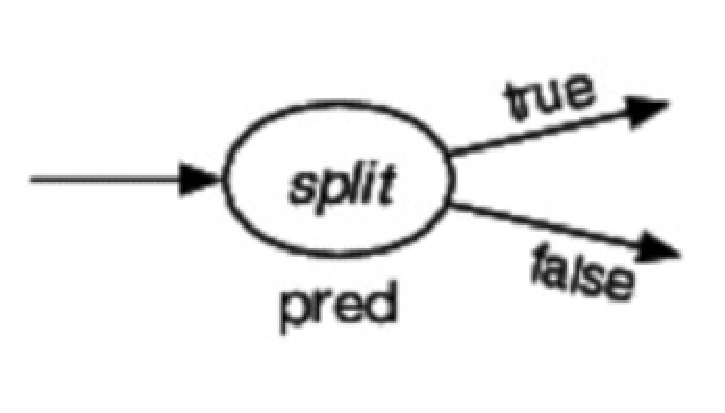
\includegraphics[width=8cm]{fig_06_003.eps}


\texttt{core.async}の \texttt{split} 関数は、1つのチャネルを受け取り、述語の真偽に基づいてトラフィックを2つの出力チャネルに分割します。これは図に示すとおりです。

例えば、\texttt{split} はストリームから無効なメッセージを分割し、別のプロセスに送って処理するのに適した方法です。


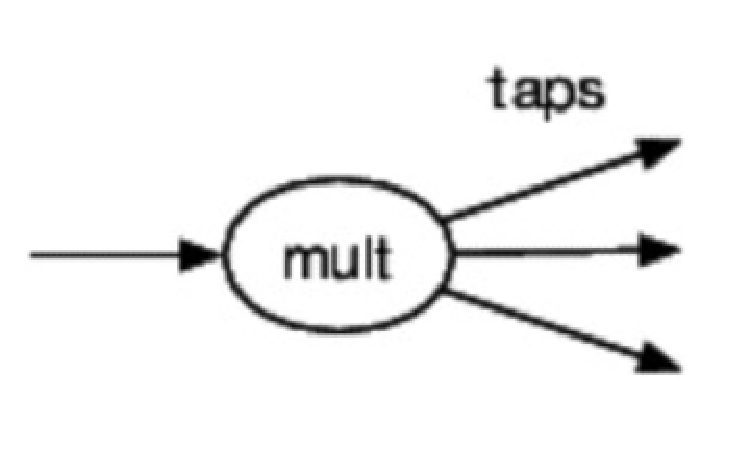
\includegraphics[width=8cm]{fig_06_004.eps}

\texttt{core.async}の \texttt{mult} 抽象化は、入力チャネルを受け取り、それを複数の出力チャネルに乗算します。

入力チャネルから項目が読み込まれると、次の値に移る前にすべての出力チャネルに供給されます。タップは \texttt{tap} 関数で \texttt{mult} に追加され(\texttt{untap} で削除され)ます。タップが閉じていることが判明した場合、そのタップは mult から削除されます。

すべてのチャネルが各値を受信する必要があるため、1つの遅いタップが \texttt{mult} を停止させる可能性があります。そこで、別のバッファリング戦略を使用することが有効です。例えば、パイプラインの特定の部分の出力ストリームをタップしてログにシャントし、何が起こっているかを覗き見ることができるようにしたいとします。

この関数は、入力と出力のチャネルを接続します( \texttt{pipe} で行ったことと同様です)が、返されるログのタップもインストールします。


\begin{lstlisting}[numbers=none]
(defn connect-and-tap
  "入力と出力を接続し、その間を流れるチャネルロギングデータを返します。"
  [input output]
  (let [m (mult input)
       log (chan (dropping-buffer 100))]
    (tap m output)
    (tap m log)
    log))
\end{lstlisting}

 % Connecting Components with Channels
\section{コンポーネントを実装する}

さて、コンポーネントをどのように呼び出し、接続するかという観点から見てきましたが、次はAPIの背後にある機能をどのように実装するかという内部事情に目を向ける必要があります。

ほとんどのコンポーネントはある種の状態を保持しており、呼び出し側がこの状態を更新したり、状態に依存する機能を呼び出したりすることができます。これまで学んできた状態のメカニズム( atom 、 ref 、 agent )は多くの方法で使用することができ、特に状態の粒度をどのように選択するかを検討します。

また、コンポーネントのライフサイクル全体についても考慮する必要があります。コンポーネントは、構成データと依存関係で構築され、内部状態や外部システムとの接続を初期化する必要があるかもしれません。コンポーネントが構築されたら、各コンポーネントを停止するためのパスも用意しておくとよいでしょう。これは、開発中にREPLで簡単に起動・停止できるようなシステムを構築するために重要です。この2つについて、さらに詳しく見ていきましょう。

まず、各コンポーネント内の状態の粒度について見ていきます。

\subsection{状態の粒度}

コンポーネントはしばしば、コンポーネントの寿命の間に変更される可能性のある実行時の状態を持っています。これはコンポーネントが管理するデータであったり、 データベース接続のような内部ステートフルリソースハンドルであったり、 あるいは動的な設定値であったりします。実行状態の初期値は設定の一部として渡されることもありますが、多くの場合、内部で構築されたり、時間の経過とともに構築されたりします。

コンポーネント内に状態を保持する場合、ステートフルなコンテナ(通常は atom か ref )を使用する必要があります。どちらを使うか、そしてステートの粒度を選択する必要がある。

主な決定要因は、必要な調整のレベルです。 atom はより単純だが、複数のステート間で調整することができない。 ref はより複雑だが、協調をサポートする。しかし、別の見方をすると、調整が必要な2つの状態の断片を1つの atom の下に持ってきて、再び1つの更新関数で対応できるようにすることも可能である。

口座のインデックスと顧客のインデックスという2種類の状態を管理する必要があるコンポーネントを考えてみましょう。これらは2つの atom として維持することができる。

\begin{lstlisting}[numbers=none]
(defrecord CustomerAccounts [accounts customers])

(defn make-customer-accounts []
  (map->CustomerAccounts {:accounts (atom {})
                          :customers (atom {})}))
\end{lstlisting}

あるいは、アカウントとカスタマーの両方でトランザクション的に変更が必要なケースであれば、 ref を使うことも可能でした。


\begin{lstlisting}[numbers=none]
(defrecord CustomerAccounts [accounts customers])

(defn make-customer-accounts []
  (map->CustomerAccounts {:accounts (ref {})
                          :customers (ref {})}))
\end{lstlisting}

ref を使用すると、コンポーネントの状態との相互作用にトランザクションを巻き付ける必要があります。その代わりに、状態の粒度を大きくして、1つの atom 内にアカウントと顧客の両方を包含することができるかもしれません。

\begin{lstlisting}[numbers=none]
(defrecord CustomerAccounts [state])

(defn make-customer-accounts []
  (map->CustomerAccounts (atom {:accounts {}
                                :customers {}})))
\end{lstlisting}

Clojureの atom は高速なので、更新関数が小さいことを前提に、その内部で粗視化された状態を使うことができる場合が多いのです。

逆に、口座や顧客を桁ごとに分割したり、名前ごとに分割してセグメントごとにrefを作成するなど、粒度をより細かくすることも可能です。コンポーネントのトップレベルの機能は影響を受けますが、エンティティレベルのデータや関数はシンプルでステートレス、そしてどのようなアプローチにも完全に再利用可能であるべきです。

\subsection{構成}

コンポーネントを実装する際には、起動時や継続的に使用するために必要な情報を保持する必要があります。コンポーネントは、構成、依存関係、実行時の状態という3つの主要な情報を必要とします。

設定データは、コンポーネントの外部で取得したり構築したりします (設定データの管理方法については、第7章 アプリケーションの構成で説明します)。作成時にコンポーネントに渡され、コンポーネントの起動時またはそれ以降に使用することができます。設定情報の一般的な使用例としては、外部リソース (データベースやメッセージシステムなど) への接続パラメータがあります。

コンポーネントを作成する際に、各設定値を個別のパラメータとして渡すことができます。

\begin{lstlisting}[numbers=none]
(defn new-component [db-url user password] ...)
\end{lstlisting}

しかし、設定データはシステムの開発に伴って変化することが多いので、設定データは必要に応じて進化できるパッケージ(マップやレコード)として渡すのがよい。

\begin{lstlisting}[numbers=none]
(defn new-component [{:keys [db-url user password]}] ...)
\end{lstlisting}

設定データだけでなく、コンポーネントが他のコンポーネントを参照する必要がある場合も多い。例えば、ナレッジエンジンコンポーネントは、設定データに加えて、データフィードコンポーネントへのアクセスを必要とする場合があります。

\begin{lstlisting}[numbers=none]
(defn new-knowledge-engine [config feed] ...)
\end{lstlisting}

しかし、あるコンポーネントを依存関係として他のコンポーネントに直接渡すよりも、それらの間にチャネルを配置することによってそれらを切り離す方が理にかなっている場合もあります。この場合、リモートコンポーネントではなく、チャネルが依存関係として扱われます。コンポーネントの接続方法を考えると、これはコンポーネントの組み立てに多くの選択肢を与えることになります。

コンポーネントには、設定、他のコンポーネントやチャネルとの依存関係、内部のランタイムの状態を保存する場所が必要です。レコードは、コンポーネントの動作を定義するプロトコルを実装するのが一般的であるため、これに最適な選択肢である。

次に、コンポーネントの状態が作成されるコンストラクションを含む、コンポーネントのライフサイクルを見ていきます。

\subsection{ライフサイクル}

ほとんどのコンポーネントのライフサイクルは単純である。最も重要なイベントは、構築、コンポーネントの開始、およびコンポーネントの停止です。

例えば、先ほどのルールベースの知識エンジンと、そのコンポーネントをどのように構築するかを考えてみましょう。議論のために、知識エンジンは受信メッセージのストリームを受け取り、ルールに従ってそれを修正し、他のコンポーネントに送信する役割を担っていることも考えてみましょう。

\begin{lstlisting}[numbers=none]
(defrecord KnowledgeEngine
  [config ;; map of config info
   ch-in ;; channel to receive messages
   ch-out ;; channel to post messages
   rules ;; state - current rule set
   active]) ;; state - true if active

(defn make-knowledge-engine
  [config ch-in ch-out rule-set]
  (->KnowledgeEngine config ch-in ch-out
          (atom rule-set) (atom false)))

(defn start-knowledge-engine
  [{:keys (ch-in ch-out rules active) :as ke}]
  (reset! active true)
  (go-loop [request (<! ch-in)
            response (fire-rules ke request)]
    (>! ch-out response)
    (when @active (recur)))
  ke)

(defn stop-knowledge-engine
  [{:keys (ch-out active) :as ke}]
  (reset! active false) ;; exit go loop
  (async/close! ch-out) ;; stop producing
  ke)
\end{lstlisting}

コンポーネントはしばしばステートフルフィールドに初期値を設定したり、その他のタスクを実行する必要があるため、通常、コンポーネントインスタンスを作成するためのカスタム関数を提供することになります。ここでは、 \texttt{make-knowledge-engine} 関数は、知識エンジンの現在のルールの状態を保持するアトムを含む、コンポーネントのインスタンスを構築します。

静的な構成は、しばしばアプリケーションの進化に伴う変更の原因となります。この進化を計画するには、静的構成を一連の位置づけの構成パラメータとしてではなく、マップとして捉えるのが最適です。これにより、頻繁に変更される設定値を、既存のコードを壊すことなく変更することができます。

\texttt{start-knowledge-engine} 関数は、受信した要求チャネルの処理を開始するためにコンポーネントをアクティブにします。軽量なgoブロックが作成され、コンポーネントの寿命まで生き続け、 \texttt{ch-in} からメッセージを抽出し、ルールを介してそれを処理し、 \texttt{ch-out} にそれを投稿します。ステートフルアクティブフラグは、ゴーブロックが継続すべきかどうかを決定するために使用されます。

\texttt{stop-knowledge-engine} 関数は \texttt{active} フラグを \texttt{false} に設定し、goブロックのループを停止させることができる。 \texttt{stop} 関数はまた、これ以上メッセージが生成されないため、出力チャネルを閉じます。入力チャネルは閉じません。その代わり、コンポーネントが停止したときに、入力チャネルのオーナーがそのチャネルをクローズする必要があります。これは \texttt{core.async} プログラムでよくある慣習です。




 % Implementing Components
\section{まとめ}

コンポーネントは、アプリケーションの実際の機能を確立する、より大きなコードの単位を構築するための手段です。コンポーネントは構造を提供し、チームが作業を分担するために使用できるコードの有意義なサブユニットを作成します。

まず、コンポーネントの外部API(関数、非同期呼び出し、チャンネルによるイベントストリーム)を設計する方法と、 core.async を使用してこれらのコンポーネントを接続する方法について見ていきました。

また、各コンポーネントの設定データ、依存関係、内部状態、コンポーネントのライフサイクルを考慮した実装方法についても見てきました。

次に、システムを組み立てるための全体像を探ります。アプリケーションの設定データをどのように管理し、コンポーネントに提供するか、コンポーネントをどのようにインスタンス化して接続するか、システムのエントリポイントをどのように提供するか、について見ていきます。 % Wrapping Up % Creating Components


\section{モノを分解する}

最初の仕事は、問題からその問題を解決するための大まかなアーキテクチャに至るまで、どのようにすればよいかを考えることです。第6章「コンポーネントの作成」で説明したように、問題を分析し、個別のコンポーネントを特定します。アプリケーション内 (あるいは複数のアプリケーションにまたがる) で汎用的なコンポーネントを再利用したり、チーム内で開発を分担したり、あるいは一度に問題の一部だけを考えることができるような構造にしたりするためです。

コンポーネントを分離する方法にルールはありませんが、いくつかの一般的なガイドラインに従うことは可能です。コードをグループ化する理由としては、関数が同じ種類のデータで動作する、データの範囲や寿命が共通である、外部要件による変更の可能性が似ている、必要なリソースが似ている、などがあります。もし、あるコードのセットが、複数のコンテキストで異なる設定をしたときに再利用可能であれば、それは間違いなく有用なコンポーネントである。

この議論を具体化するために、次のような問題を考えてみよう。私たちの会社は、ソーシャルメディア上の製品に関する言及を監視し、それに対応できるシステムを必要としています。その応答は、タイムリーで、有用で、適切であることが重要である。この役割を果たす人はいますが、当社の製品は非常に人気があるため、注意が必要なメッセージを見つけ、回答候補を作成し、その回答を送信するというプロセスを自動化するための支援が必要です。

この問題を考えているうちに、アプリケーションにいくつかの境界線が見えてきました。ソーシャルメディアフィードの監視を自動化する場合、各サードパーティシステムとのやり取りをカプセル化するコンポーネントが必要です。これらのフィードは、個々のシステムとのやり取りは別々であっても、それ自体は多くの類似した実装ニーズを共有することができます。フィードは、外部リソースを使用し、そのライフサイクルをフィードに結合しているため、別個のコンポーネントとなります。

同様に、メッセージにどのように応答するかというルールの知識ベースをカプセル化するコンポーネントが必要になります。これは自己完結型でも、外部システムを使ってルールを呼び出すことも可能です。

最後に、元のメッセージと応答候補を受け取り、それらをソーシャルメディアの専門家に提示して、メッセージを承認するか修正するかを決定するコンポーネントが必要になると思われます。このコンポーネントは、ある人物へのアクセスを処理する役割を担っています。

アーキテクチャとそのハイレベルなコンポーネントがどのようなものかは、スケッチでご覧いただけます。 

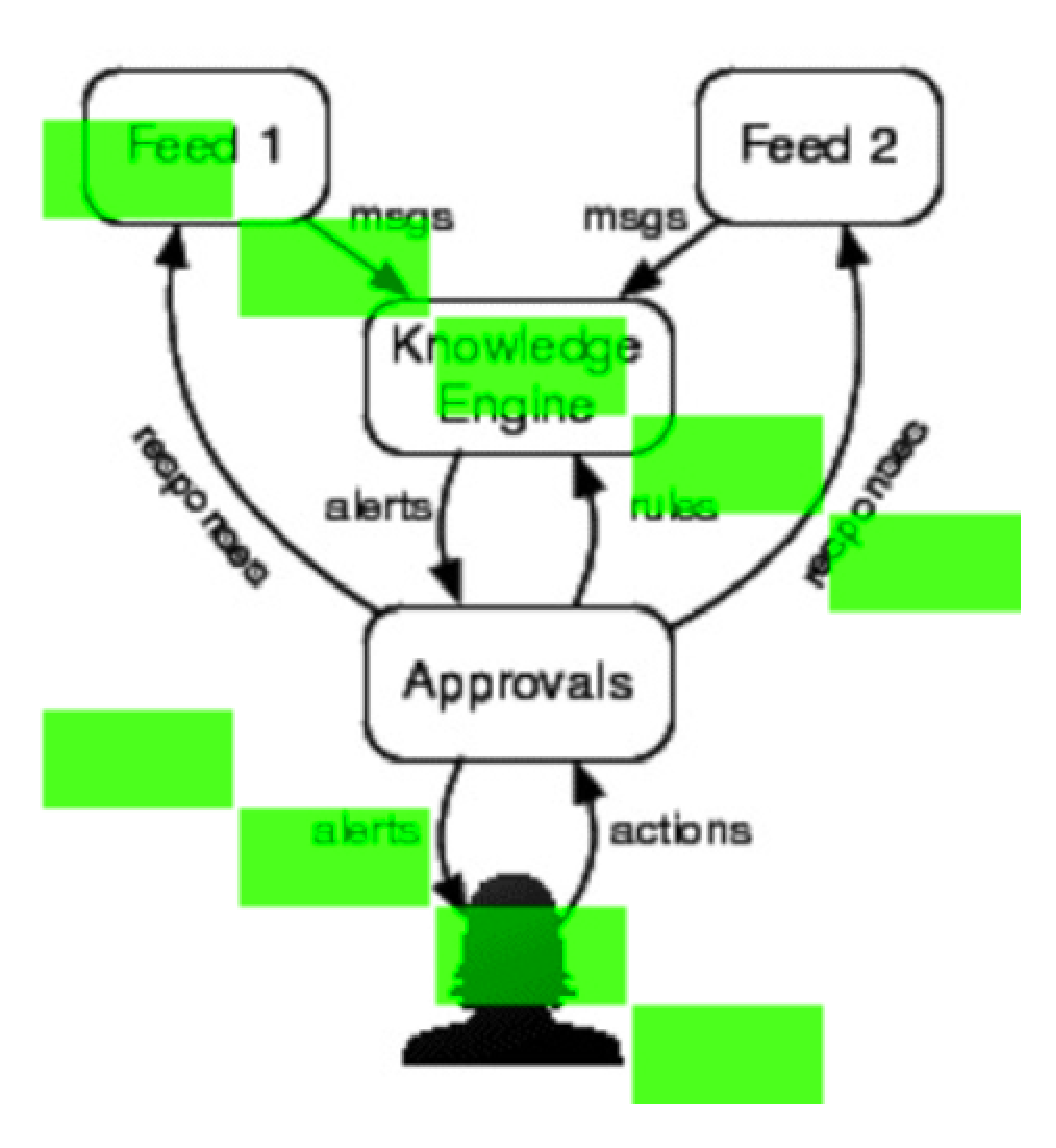
\includegraphics[width=8cm]{fig_07_001.eps}

次に、必要となるコンポーネントを定義し、それらをどのように接続するかを考えてみましょう。システムを組み立てていく上で、アプリケーションやコンポーネントのライフサイクルを考慮する必要がある。Clojureでこのような問題に最適なライブラリはComponentです\[20\]。コンポーネントを定義しながら、Componentを介してライフサイクルの開始と停止の機能を設定します。









 % Taking Things Apart
\section{Componentを用いた実装}

各コンポーネントについて、必要な構成、実行時の状態、他のコンポーネントとの接続を考慮する必要があります。コンポーネントとそのライフサイクルメソッドを定義したら、コンポーネントをどのように組み立てて実行システムにするかを見ていきましょう。

まず、ソーシャルメディアのフィードから始めましょう。各フィードには、そのフィードに接続するための認証設定が必要です。システムによっては、ユーザー名やパスワード、その他のアクセスキーが必要になります。また、フィードをアクティブにするか一時停止するかという実行時の状態も維持することになります。最後に、新しいメッセージを core.async チャネルでプッシュし、送信メッセージを別のチャネルで受信することを想定しています。このような情報を持つレコードとして、コンポーネントを定義します。


\begin{lstlisting}[numbers=none]
(defrecord Feed [auth status msg-chan response-chan])

(defn new-feed [auth msg-chan response-chan]
  (->Feed auth (atom :init) msg-chan response-chan))
\end{lstlisting}

最初の\texttt{auth}フィールドは、フィードタイプに指定された認証情報のマップを含む。\texttt{status}は、変化する実行時の状態です(アトムに保持されます)。最後の2つのフィールドは、メッセージの送信と受信に使用する実行時チャネルです。これらは起動時に接続され、その後変更されることはありません。

次に、\texttt{component/Lifecycle} プロトコルを実装してフィードの定義を拡張する必要があります。まず、Component をプロジェクトに追加し、以下の依存関係を設定します。

\begin{lstlisting}[numbers=none]
[com.stuartsierra/component "0.2.3"]
\end{lstlisting}

次に、名前空間に以下のrequireを追加します。

\begin{lstlisting}[numbers=none]
[com.stuartsierra.component :as component]
\end{lstlisting}

そして、コンポーネントの開始と停止のための2つのメソッドだけを持つ、\texttt{component/Lifecycle}プロトコルを拡張することができるようになりました。

\begin{lstlisting}[numbers=none]
(defrecord Feed [auth status msg-chan response-chan]
  component/Lifecycle
  (start [component]
    (reset! (:status component) :running)
    (process-messages status msg-chan)
    (handle-responses status response-chan)
    component)
  (stop [component]
    (reset! (:status component) :stopped)
    component))
\end{lstlisting}

\texttt{start}関数は、コンポーネントの状態を\texttt{:running}に設定し、受信メッセージを\texttt{msg-chan}に流す処理を開始し、応答を\texttt{response-chan}のフィードに戻す処理を開始します。サブプロセスはいずれもステータスを受け取り、ステータスが\texttt{:running}から変化したときに自分自身を停止させることができます。最後に、この関数は残りの起動のために同じコンポーネントのインスタンスを返します。

\texttt{stop}関数はステータスを\texttt{:stopped}に設定するだけです。残りの部分はサブプロセスが処理します。

次に、ナレッジエンジンコンポーネントを考えてみましょう。知識エンジンは、ルールの外部データベースに対する認証情報と、使用するルールセットで構成されます。実行時の状態は、外部のルール・データベースへの接続で構成されます。また、このコンポーネントにはフィードコンポーネントからの受信チャンネルと、承認コンポーネントへの送信フィードが必要です。

\begin{lstlisting}[numbers=none]
(defrecord KnowledgeEngine
  [ke-config feed-chan alert-chan rules]
  component/Lifecycle
  (start [component]
    (watch-feeds feed-chan alert-chan)
    component)
  (stop [component]
    component))

(defn new-knowledge-engine
  "初期ルールのない新しい知識エンジンを作成する"
  [ke-config feed-chan alert-chan]
  (->KnowledgeEngine ke-config feed-chan alert-chan
                     (atom (:rule-set ke-config))))
\end{lstlisting}

\texttt{KnowledgeEngine} コンポーネントは、コンポーネント構成データ、受信 \texttt{feed-chan} 、送信 \texttt{alert-chan} を保持するための \texttt{ke-config} を持ちます。さらに、この実装では、内部 \texttt{rules} を持ちます。これは、コンストラクタで公開されない実装の詳細です。他の実装では、外部のデータベースやルールシステムでルールを管理することができます。

知識エンジンの \texttt{start} 関数は、送られてくるフィードを監視し、ルールを処理し、必要と判断されればアラートチャンネルでアラートメッセージを発するプロセスをセットアップします。\texttt{stop} 関数は特別なことをする必要はありませんが、サブプロセスを停止させることは可能です。

知識エンジンは、ルールセットを管理するために、承認コンポーネントから直接呼び出すことができるAPIを持っています。回答を承認する人は、ナレッジエンジンから出力される内容に基づいてルールを追加、修正、削除することもでき、最終的にシステム全体を向上させることができます。ルールを追加するためのAPI関数の例は次のとおりです。

\begin{lstlisting}[numbers=none]
(defn add-rule
  "セットへのルール追加"
  [ke rule]
  (swap! (:rules ke) conj rule))
\end{lstlisting}

\texttt{add-rule}のようなコンポーネント関数は、通常、第一引数としてコンポーネントを取る通常の関数です。知識エンジンのインスタンスが承認コンポーネントに注入されると、そのコンポーネントはこれらの関数を直接呼び出すことができるようになります。

最後に、承認(approvals)コンポーネントを検証する必要がある。このコンポーネントは、アラートが発生した場合に適切な人にメールを送信するためのいくつかの設定を持っています。アラート・チャネルで受信したメッセージを、電子メールや他の通知システムで適切な人に転送する。応答は応答チャネルで受信し、フィードに送り返す応答や、 将来この種のメッセージをどのように処理するかについて知識エンジンに 追加する新しいルールを含むことができます。

\begin{lstlisting}[numbers=none]
(defrecord Approvals
   [approval-config ;; 承認コンフィグ
    alert-chan ;; 受信アラートメッセージ
    knowledge-engine ;; ナレッジエンジンへの直接フック
    response-chan] ;; 出力応答メッセージ pub/sub
  component/Lifecycle
  (start [component]
    (process-alerts alert-chan)
    (process-responses knowledge-engine
                       response-chan)
    component)
  (stop [component]
    component))
  (defn new-approvals
    [approval-config alert-chan response-chan]
    (map->Approvals {:approval-config approval-config
                     :alert-chan      alert-chan
                     :response-chan response-chan}))
\end{lstlisting}

なお、\texttt{Approvals}コンポーネントは、コンポーネントが適切に起動し、呼び出される前に知識エンジンが注入されることを想定しています。

さて、すべてのコンポーネントが揃ったところで、それらを組み立てるためにコンポーネントシステムを使用する必要があります。

 % Implementing with Component
\section{物事をまとめる}

Componentでは、システムは他のコンポーネントを起動したり停止したりできる特別なコンポーネントである。システム内のコンポーネントは、依存関係が常にコンポーネントの前に開始されるような順序で開始される。このため、コンポーネントの依存関係グラフにサイクルが存在しないことが必要である。同様に、システムが停止されるとき、コンポーネントは開始と逆の順序で停止される。

システムは、\texttt{component/system-map}関数で定義される。マップは、コンポーネント名からコンポーネントインスタンスへのマッピングを定義する。コンポーネントがコンポーネントの依存関係を持つ場合、これは \texttt{component/using} で指定され、注入されたコンポーネントのベクトル(システム内とコンポーネント内で名前が同じ場合)またはコンポーネント名からシステム名へのマッピングのいずれかを取ります。

この関数は、システムで定義したコンポーネントから、コンポーネントシステムマップを作成します。

\begin{lstlisting}[numbers=none]
(defn system [{:keys (twitter facebook knowledge approvals) :as config}]
  (let [twitter-chan (async/chan 100)
        twitter-response-chan (async/chan 10)
        facebook-chan (async/chan 100)
        facebook-response-chan (async/chan 10)
        alert-chan (async/chan 100)
        response-chan (async/chan 100)
        feed-chan (async/merge [twitter-chan facebook-chan])
        response-pub (async/pub response-chan :feed)]
    (async/sub response-pub :twitter twitter-response-chan)
    (async/sub response-pub :facebook facebook-response-chan)
    (component/system-map
      :twitter (feed/new-feed twitter twitter-chan twitter-response-chan)
      :facebook (feed/new-feed facebook facebook-chan facebook-response-chan)
      :knowledge-engine
        (kengine/new-knowledge-engine knowledge feed-chan alert-chan)
      :approvals (component/using
                   (approvals/new-approvals approvals alert-chan response-chan)
                   [:knowledge-engine]))))
\end{lstlisting}

\texttt{system} 関数の最初の部分では、システムに必要な \texttt{core.async} チャネルとその他のチャネルパイプをすべて作成します。次に \texttt{component/system-map} 関数で、4つのコンポーネントとその構成、そしてナレッジエンジンを承認コンポーネントに注入する方法を定義しています。最後に、システムマップと承認コンポーネント自体で名前が一致する1つのコンポーネントのベクトルで、 \texttt{component/using} の使い方を示しています。

各コンポーネントには、コンポーネントを起動したり、その動作に影響を与えるために必要な設定情報があります。ほとんどのアプリケーションは、多くの構成要素を持つことになります。次に、開発から配備までの完全なライフサイクルをサポートする方法で、アプリケーションに設定データをロードする方法を見てみましょう。







 % Putting Things Together
\section{システム構成}

システム構成には、システム属性、環境ごとの情報、開発者専用の情報など、いくつかの種類の設定が含まれています。システム属性とは、アプリケーションの動作に影響を与えるフラグやその他の設定のことで、機能のオン・オフや、いつか変更する必要のあるマジックナンバーを外部化することができます。環境ごとの情報は、開発、品質保証、本番など、アプリケーションの展開先ごとに変化します。そして最後に、開発者専用の設定は、開発者が作業中に自分のマシン上で環境を微調整することを可能にします。

これらの設定のうち、ソースコントロールにチェックできるのはシステム属性のみです。環境ごとの設定は、アプリケーションの外側の環境で設定する必要があります。dev- onlyの設定は、個々の開発時にローカルにのみ設定されるべきものです。

起動時に、これらすべての種類の値をまとめて、システム設定の一貫したビューにロードする必要があります。ここでは、複数のソースから取得した値に対する一貫したインターフェースを得るための一つの方法として、Environライブラリについて見ていきます。もう少し深い解決策としては、Immuconf ライブラリを利用することにします。

\subsection{Environ}

Environライブラリは、Leiningenプロファイル、環境変数、およびJavaシステムプロパティから取得した設定値を一元的に表示するものです。\texttt{:rule-set}(使用する知識エンジンのルールセット)、\texttt{:feed1-user}(ソーシャルメディアのフィードのユーザー名)、\texttt{:verbose}(開発時のデバッグフラグ)の3つのシステム構成プロパティを考えてみましょう。

開発時には、ローカルビルドで\texttt{rule-set}と\texttt{feed1-user}を設定したいと思うかもしれません。Environでこの設定を行うには、まずLeiningenの\texttt{project.clj}を更新して、Environを依存関係として(コードに)、lein-environプラグインを(ビルドに)追加する必要があります。


\begin{lstlisting}[numbers=none]
:dependencies [[environ "1.0.0"]]
:plugins [[lein-environ "1.0.0"]]
\end{lstlisting}

システム構成プロパティを設定する最初の場所は、\texttt{project.clj} の中で Leiningen プロファイルの一部として直接設定することができます。プロファイルを使用すると、プロジェクトのビルドにオプションで含まれるプロジェクト設定のバンドルを作成することができます。プロファイルの一般的な使い方の1つは、環境固有のプロジェクト環境を作成することです。Leiningen では、プロファイル名とプロファイル固有のプロジェクト設定のマップを含む \texttt{:profiles} キーを使用します。

\begin{lstlisting}[numbers=none]
:profiles {:dev  { ,,, }
           :qa   { ,,, }
           :prod { ,,, }}
\end{lstlisting}

Environライブラリは、プロジェクト設定にある\texttt{:env}キーからシステム設定を読み込むことを想定しています。

\begin{lstlisting}[numbers=none]
:profiles {:dev {:env {:rule-set "basic"}}
           :prod {:env {:rule-set "advanced"}}}
\end{lstlisting}

Leiningenでは \texttt{:user} と \texttt{:dev} のプロファイルはよく知られていて、デフォルトでオンになっているので、\texttt{lein repl}でいつも通りREPLを起動すれば、devの設定が利用できるようになります。

\begin{lstlisting}[numbers=none]
user=> (require '[environ.core :refer (env)])
nil
user=> (env :rule-set)
"basic"
\end{lstlisting}

しかし、\texttt{project.clj}ファイルは、通常、ソースコントロールシステムで追跡されます。\texttt{:rule-set}のような環境設定は問題ありませんが、別の構成設定(データベースのユーザー名とパスワードなど)はおそらく受け入れられません。その場合、開発者固有の設定として、ソース・コントロールの外にある別の Leiningen \texttt{profiles.clj} に設定を保存することをお勧めします。

この例では、\texttt{project.clj} から \texttt{:profiles} を削除し、代わりに \texttt{profiles.clj} の中に \texttt{:profiles} キーの値を入れることで、この例を変更することができます。


\begin{lstlisting}[numbers=none]
{:dev {:env {:rule-set "basic"}}
 :prod {:env {:rule-set "advanced"}}}
\end{lstlisting}


 % System Configuration
\input{002-007-005.tex} % Wrapping Up % Compose Your Application

\part{実践編}
\part{付録}
\end{document}


\begin{itembox}[l]{実質的に一定時間}
\end{itembox}

\begin{enumerate}
\item
\end{enumerate}

\begin{itemize}
\end{itemize}

\begin{description}
\end{description}

\begin{lstlisting}[numbers=none]

\end{lstlisting}


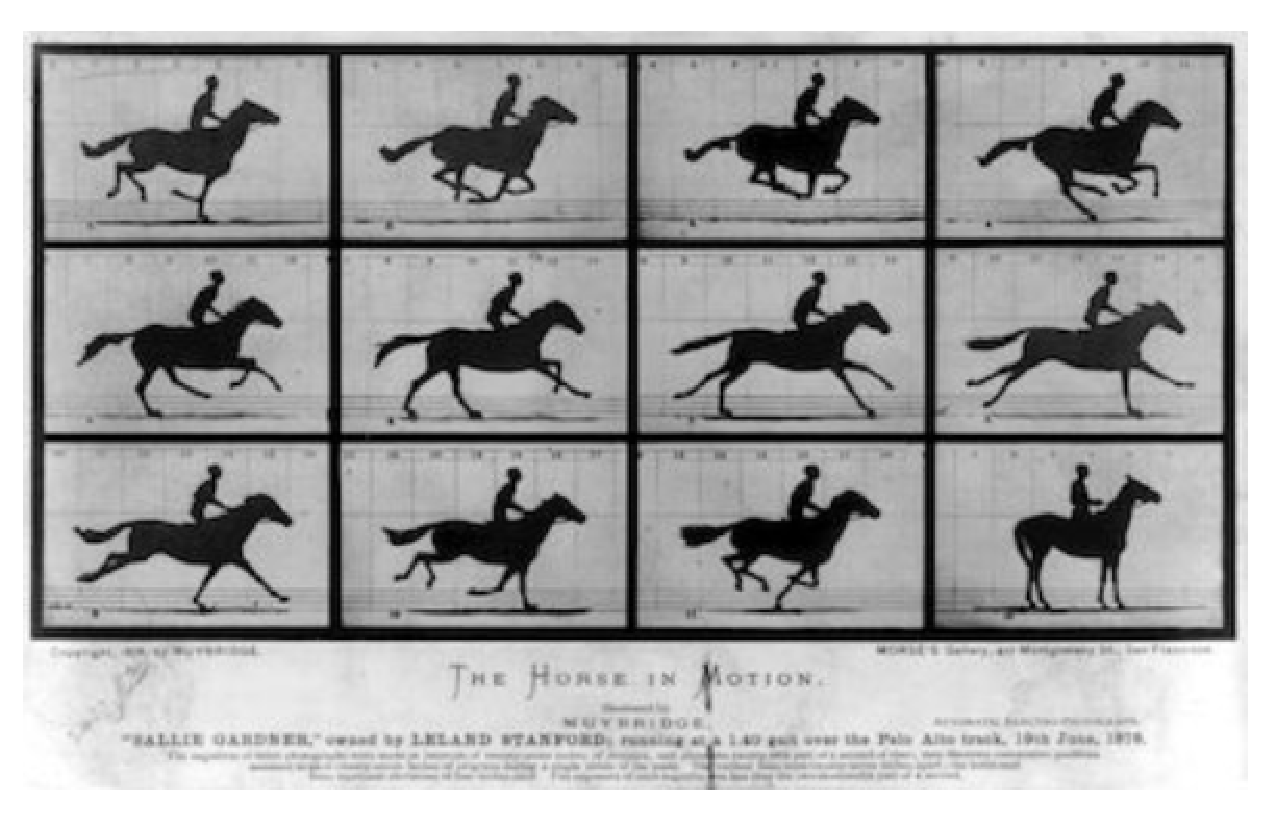
\includegraphics[width=10cm]{fig_04_001.eps}